\documentclass[12pt,italian]{report}
\usepackage{tesi}

%
%			INFORMAZIONI SULLA TESI
%			DA COMPILARE!
%

% CORSO DI LAUREA:
\def\myCDL{Corso di Laurea Magistrale in Informatica}

% TITOLO TESI:
\def\myTitle{Analisi di dati multi-omici per la predizione\\ \vspace{0.4cm} della prognosi di pazienti oncologici}

% AUTORE:
\def\myName{Alessandro Beranti}
\def\myMat{Matr. Nr. 977702}

% RELATORE E CORRELATORE:
\def\myRefereeA{Prof. Elena Casiraghi}
\def\myRefereeB{Prof. Dario Malchiodi}

% ANNO ACCADEMICO
\def\myYY{2021-2022}

% Il seguente comando introduce un elenco delle figure dopo l'indice (facoltativo)
%\figurespagetrue

% Il seguente comando introduce un elenco delle tabelle dopo l'indice (facoltativo)
%\tablespagetrue

%
%			PREAMBOLO
%			Inserire qui eventuali package da includere o definizioni di comandi personalizzati
%

% Package di formato
\usepackage[a4paper]{geometry}		% Formato del foglio
\usepackage[italian]{babel}			% Supporto per l'italiano
\usepackage[utf8]{inputenc}			% Supporto per UTF-8
\usepackage[a-1b]{pdfx}			% File conforme allo standard PDF-A (obbligatorio per la consegna)
%\usepackage[pdfa]{hyperref}

% Package per la grafica
\usepackage{graphicx}				% Funzioni avanzate per le immagini
\usepackage{hologo}					% Bibtex logo with \hologo{BibTeX}
%\usepackage{epsfig}				% Permette immagini in EPS
\usepackage{xcolor}				% Gestione avanzata dei colori

% Package tipografici
\usepackage{amssymb,amsmath,amsthm} % Simboli matematici
\usepackage{listings}				% Scrittura di codice

% Package ipertesto
%\usepackage{url}					% Visualizza e rendere interattii gli URL
%\usepackage{hyperref}				% Rende interattivi i collegamenti interni
\usepackage{caption}
\usepackage{booktabs}
\usepackage{cite}
\usepackage{verbatim}
\usepackage{setspace}
\onehalfspacing 
\usepackage{adjustbox}
\usepackage{makecell}
\usepackage{colortbl}
\lstset{language=Python}
\usepackage{quoting}
\usepackage{caption}
\usepackage{subcaption}
\quotingsetup{font=small}


\begin{document}
	
	% Creazione automatica del frontespizio
	\frontespizio
	\beforepreface
	
	% 
	%			PAGINA DI DEDICA E/O CITAZIONE
	%			facoltativa, questa è l'unica cosa che dovete formattare a mano, un po' come vi pare
	%
	
	{\raggedleft \large \sl Alla mia famiglia\\
		Oriella, Andrea e Giuseppe\\
		
	}
	
	
	
	
	% 
	%			PREFAZIONE (facoltativa)
	%
	
	%\prefacesection{Prefazione}
	%Le prefazioni non sono molto comuni, tuttavia a volte capita che qualcuno voglia dire qualcosa che esuli dal lavoro in s\'e (come un meta-commento sull'elaborato), o voglia fornire informazioni riguardanti l'eventuale progetto entro cui la tesi si colloca (in questo caso \`e probabile che sia il relatore a scrivere questa parte).
	
	%
	%			RINGRAZIAMENTI (facoltativi)
	%
	
	\prefacesection{Ringraziamenti}
	Un grazie sincero a Oriella, Andrea e Giuseppe che mi hanno sempre supportato. Grazie agli amici che mi sono stati vicini, in particolare ai miei compagni di corso Andrea e Samuele con cui ho condiviso tutto percorso magistrale. Infine un sincero ringraziamento ai miei relatori Elena Casiraghi e Dario Malchiodi.
	Grazie a tutti.
	
	%
	%			Creazione automatica dell'indice
	%
	
	\afterpreface
	
	
	% 
	%			CAPITOLO 1: Introduzione o Abstract
	% 
	
	\chapter*{Introduzione}
	\addcontentsline{toc}{chapter}{Introduzione}
	\markboth{Introduzione}{Introduzione}
	\label{cap:introduzione}
	Il \textit{machine learning} è sempre più diffuso in molti ambiti diversi. L'idea di poter usare questa tecnologia anche in campo medico è affascinante poiché potrebbe permettere di riuscire a migliorare prevenzione, diagnosi e monitoraggio delle malattie. Grazie all'uso di dati provenienti da pazienti è possibile creare modelli di \textit{machine learning} esattamente con questi scopi. In questo lavoro è stato usato apprendimento supervisionato usando \textit{random forest} come algoritmo di classificazione poiché è noto, in letteratura, per essere uno dei metodi migliori quando si hanno dati eterogenei. L'obiettivo è quello di usare dati provenienti dai geni BRCA per predire la prognosi e diagnosi di pazienti al carcinoma mammario invasivo. In particolare si vuole verificare se l'utilizzo di dati multi-omici riesca ad aumentare l'accuratezza della previsione.
	I geni BRCA1 e BRCA2 sono geni importanti per la salute dei tessuti della mammella e dell'ovaio. Questi geni sono normalmente responsabili della produzione di proteine che proteggono dalle mutazioni del DNA e prevengono la crescita di cellule anormali.
	Tuttavia, quando i geni BRCA1 e BRCA2 sono mutati, le proteine che producono non funzionano correttamente e c'è un rischio maggiore di sviluppare tumori del seno e dell'ovaio.
	
	I dati a disposizione sono dati multi-omici, ovvero un insieme che contiene le variazioni molecolari su più livelli quali: genomica, epigenomica, trascrittomica, proteomica, metabolomica e microbiotica.
	Grazie alla ricerca ci sono stati importanti progressi in diversi campi omici e si è capito che la risposta a una domanda in medicina non è solo da ricercare in un unico tipo di dato poiché questi dati si influenzano tra loro. 
	
	Il lavoro è composto da quattro capitoli. Nel Capitolo \ref{statoArte} viene affrontato il concetto di \textit{machine learning} illustrando le varie tipologie di apprendimento possibili, entrando più nel dettaglio per quanto riguarda l'apprendimento supervisionato e, in particolare, approfondendo i \textit{random forest}, ovvero l'algoritmo di classificazione usato durante gli esperimenti. Vengono inoltre analizzate due soluzioni presenti in letteratura, in cui si è applicato il paradigma \textit{machine learning} per problemi medici.
	Nel Capitolo \ref{Dataset} viene discussa la fonte e la struttura dei dati. Vengono inoltre esaminate le fasi appartenenti al \textit{preprocessing} che possono essere seguite per rendere i dati più qualitativi. Infine vengono trattate le tecniche di riduzione della dimensionalità utilizzate durante gli esperimenti. 
	Nel Capitolo \ref{Esperimenti} vengono illustrati i passi di \textit{preprocessing} usati sul \textit{dataset} fornito, il processo di \textit{model selection}, la metrica di \textit{performance} usata e infine tutti gli esperimenti effettuati con i relativi risultati ottenuti.
	Per ultimo, nel Capitolo \ref{Conclusioni}, vengono discusse le conclusioni sul lavoro ed eventuali possibili sviluppi futuri.
	
	\chapter{Stato dell'arte}
	\label{statoArte}
	\section{Machine Learning}
	Il termine \textit{Machine Learning}, anche chiamato apprendimento automatico in italiano, sta a indicare la capacità dei computer di apprendere e adattarsi agli input forniti.
	Molto spesso tale termine viene utilizzato per intendere l'Intelligenza Artificiale e viceversa ma non sono la stessa cosa: il \textit{Machine Learning} è un sottoinsieme della categoria più ampia chiamata appunto Intelligenza Artificiale.
 
	L'intelligenza artificiale può essere definita come la branca dell'informatica che si occupa dell'automazione del comportamento intelligente \cite{luger2005artificial}. Tuttavia 
	è importante che sia definito in modo chiaro cosa significhi intelligenza. Sebbene la maggior parte di noi sia certa di poter riconoscere un comportamento intelligente quando lo vede, non è certo che chiunque possa avere una definizione chiara di intelligenza per poter valutare un programma informatico come intelligente o meno.
	L'intelligenza artificiale si concentra sullo sviluppo di sistemi in grado di eseguire compiti per cui è richiesta l'intelligenza umana, come il ragionamento, l'apprendimento, la comprensione del linguaggio naturale e la percezione visiva. L'aspetto ``intelligente'' dell'intelligenza artificiale si basa sull'abilità che hanno i sistemi di adattarsi e migliorare continuamente in base a nuovi stimoli (dati) che ricevono, imitando, in qualche modo, il processo di apprendimento dell'essere umano.
	Di seguito vengono illustrati esempi particolarmente recenti di questi sistemi. 
	\begin{itemize}
		\item Assistenti virtuali, come \textit{Siri} o \textit{Alexa}, ovvero agenti software in grado di eseguire azioni o erogare servizi in base a comandi ricevuti in maniera vocale o testuale. Esistono sistemi simili, anche chiamati \textit{Chatbot} \cite{lalwani2018implementation}, che vengono utilizzati nel \textit{Customer Care} aziendale come primo livello di assistenza con il cliente. Si contraddistinguono per la loro capacità di comprensione del tono del dialogo e di memorizzazione delle informazioni raccolte. Essi sono sistemi di raccomandazione che indirizzano le scelte degli utenti in base a informazioni fornite da essi: famosi sono quelli che suggeriscono un acquisto in base a quelli fatti in precedenza.
		
		\item Il \textit{Natural Language Processing} (NLP), ramo dell’intelligenza artificiale che riguarda l’informazione espressa nel linguaggio naturale. Si tratta di sistemi che elaborano il linguaggio, con finalità che possono variare dalla comprensione del contenuto, alla traduzione, fino alla produzione di testo in modo autonomo a partire da dati o documenti forniti in input \cite{cambria2014jumping}.
		
		\item La \textit{Computer Vision}, area dell'intelligenza artificiale che si occupa di creare macchine che siano i grado di ``vedere''. In questo contesto però tale termine significa essere in grado di estrapolare informazioni da una o più immagini per risolvere un particolare compito \cite{DANUSER2011973}. I sistemi di \textit{Computer Vision} vengono implementati in una vasta gamma di applicazioni, sia industriali che scientifiche, tra cui sistemi per il controllo di robot e veicoli autonomi, sorveglianza video, diagnostica medica, riconoscimento di persone e oggetti, lettura di testo e misurazione di proprietà geometriche \cite{szeliski2022computer}.
		
		\item La diagnosi medica, sistemi che sfruttano l'intelligenza artificiale per analizzare immagini e usare dati medici in modo da aiutare la diagnostica di malattie.
		\item L' analisi dei dati, sistemi che utilizzano l'intelligenza artificiale per analizzare grandi quantità di dati e ottenere informazioni utili per prendere decisioni, per esempio in campo aziendale.
	\end{itemize}
	Il \textit{Machine Learning} è un campo di ricerca che si concentra sulla costruzione di metodi che ``apprendono'', ovvero sistemi in grado di migliorare le proprie prestazioni in un compito attraverso l'esperienza \cite{10.5555/541177}. Più precisamente: un programma informatico si dice che impara dall'esperienza $E$ rispetto a una classe di compiti $T$ e una misura di prestazioni $P$, se le sue prestazioni nei compiti in $T$, misurate da $P$, migliorano con l'esperienza $E$ \cite{10.5555/541177}.
	Ad esempio, un programma informatico che impara a giocare a dama potrebbe migliorare le sue prestazioni misurate dalla sua capacità di vincere nella classe di compiti di giocare a partite di dama, attraverso l'esperienza ottenuta giocando contro se stesso.	
	
	Un algoritmo di \textit{Machine Learning} è una procedura, o una serie di istruzioni, che vengono eseguite sui dati con l'obiettivo di creare un modello. Un modello di \textit{Machine Learning} è il risultato finale dell'applicazione di un algoritmo di \textit{Machine Learning} a un insieme di dati di \textit{training}.
	Gli algoritmi di apprendimento automatico costruiscono un modello basato sui dati, noti come \textit{training data}, al fine di effettuare previsioni o decisioni senza essere esplicitamente programmati per farlo\footnote{``Senza essere esplicitamente programmati per farlo'' è una definizione attribuibile a Arthur Samuel, colui che coniò il termine \textit{Machine Learning} nel 1959.}. 
	Gli algoritmi vengono divisi in quattro categorie distinte a seconda del tipo di dato usato per eseguire la fase di apprendimento. Di seguito sono elencate le categorie:
	\begin{itemize}
		\item supervised learning,
		\item non supervised learning,
		\item semi-supervised learning,
		\item reinforced learning.
	\end{itemize}
	
	\subsection{Supervised Learning}
	\label{SupervisedLearning}
	Nel \textit{Supervised Learning}, anche chiamato apprendimento supervisionato in italiano, si ha un insieme di dati $X$ chiamato \textit{training set} composto da $N$ coppie di \textit{input-output}, \{$(x_1, y_1), (x_2, y_2),...,(x_N, y_N)$\} dove ogni $y_j$ è stata generata da una funzione sconosciuta $y=f(x)$. Lo scopo è trovare la funzione $h$ che meglio approssima la funzione $f$ \cite{russell2010artificial}.
	Imparare non è altro che la ricerca, all'interno dello spazio delle possibili ipotesi, della funzione che meglio approssima la funzione di partenza. Per misurare l'accuratezza di un'ipotesi passiamo alla funzione trovata un \textit{test set} di esempi diversi dal \textit{training set}. Un \textit{training set} non è altro che un insieme di dati utilizzato per addestrare il modello di \textit{Machine Learning}. Un \textit{test set}, invece, è un insieme di dati che non è stato usato durante la fase di addestramento. Possiamo dire che un modello generalizza bene se prevede correttamente il valore di $y$ per gli esempi che non ha usato durante la fase di addestramento.
	
	Quando l'\textit{output} $y$ è un valore di un insieme finito (come per esempio \{soleggiato, piovoso, nuvoloso\}), il problema di apprendimento è chiamato classificazione; in particolare si dice binaria o booleana se ci sono solo due valori nell'insieme. Questi tipi di valori si dicono anche categorici, essi sono variabili discrete e di norma sono privi di un ordine.
	Al contrario, quando $y$ è un numero, come per esempio la temperatura atmosferica, il problema di apprendimento è chiamato regressione. Questo tipo di valore è chiamato numerico e può essere rappresentato da un numero reale continuo come da uno discreto.
	
	All'interno di \textit{supervised learning} un problema ricorrente è l'\textit{overfitting}. È molto facile costruire un modello che si adatta perfettamente al \textit{training set} ma potrebbe essere poi incapace di generalizzare bene su dati che non ha usato durante l'addestramento.
	Per valutare la capacità di generalizzazione di un modello vengono usati dati provenienti dalla stessa popolazione di dati usati per costruire il modello. Questo viene solitamente fatto utilizzando metodi di ricampionamento di dati, come la \textit{cross-validation} \cite{berrar2019cross}.
	Di seguito vengono illustrate diverse strategie per effettuare la \textit{cross-validation}.
	\begin{itemize}
		\item \textit{K-fold cross-validation}: i dati vengono divisi in $k$ \textit{fold} o gruppi. Il modello viene addestrato usando $k-1$ sottoinsiemi, che uniti costituiscono il \textit{training set}. Successivamente il modello è applicato al sottoinsieme rimanente che viene chiamato \textit{validation set} e viene misurata la performance.
		Questo processo viene ripetuto finché ognuno dei $k$ sottoinsiemi non è stato usato come \textit{validation set}. Infine la \textit{performance} del modello viene calcolata come media delle \textit{performance} ottenute a ogni iterazione. Un esempio è visibile in Figura \ref{fig:cross-validation}.	
		
		\begin{figure}[h]
			\centering
			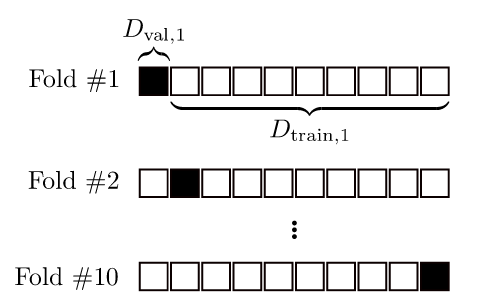
\includegraphics[width=0.7\linewidth]{immagini/cross-validation}
			\caption{\textit{10-fold cross-validation}. L'insieme di dati, $D$ è randomicamente diviso in 10 sottoinsiemi disgiunti, ognuno dei quali contiene, approssimativamente, il 10\% dei dati. Il modello è addestrato usando il \textit{training set} ($D_{train}$) e successivamente applicato al \textit{validation set} ($D_{val}$) (fonte: \cite{berrar2019cross}).}
			\label{fig:cross-validation}
		\end{figure}
		\item \textit{Leave-one-out cross-validation}: speciale caso della \textit{k-fold cross-validation} in cui $k=n$. È un metodo di validazione di un modello di \textit{Machine Learning} che consiste nel prendere un solo elemento del \textit{dataset} e utilizzarlo come \textit{test set}, il resto dei dati viene invece usato come \textit{training set}. Questa operazione viene ripetuta per ogni elemento del \textit{dataset}. In questo modo, ogni elemento viene utilizzato una sola volta come \textit{test set} e il modello viene addestrato sui dati restanti. Il costo computazionale di questa tecnica può essere elevato per grandi insiemi di dati. Tecnica visibile in Figura \ref{fig:leave-one-outcrossvalidation}.
		\begin{figure}[h]
			\centering
			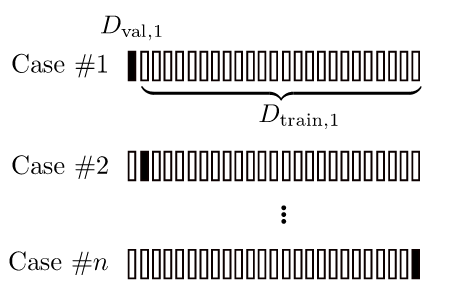
\includegraphics[width=0.7\linewidth]{immagini/leave-one-out_cross_validation}
			\caption{\textit{Leave-one-out cross-validation} applicata su un insieme di dati con  $n=25$ casi. Ogni caso funge da singolo caso di test. Il modello è costruito usando i restanti $n-1$ casi (fonte: \cite{berrar2019cross}).}
			\label{fig:leave-one-outcrossvalidation}
		\end{figure}		
	\end{itemize}
	\label{Overfitting}
	Con il termine \textit{overfitting}, o sovradattamento in italiano, si intende l'utilizzo di modelli o procedure che violano il principio di parsimonia, anche noto come rasoio di Occam\footnote{Il rasoio di Occam è un principio metodologico che sostiene che, tra le varie spiegazioni possibili per un fenomeno, quella più semplice è probabilmente la più corretta. In altre parole, si dovrebbe scegliere la spiegazione più semplice, tra quelle disponibili, per un fenomeno in quanto essa ha meno probabilità di contenere errori o di essere falsa.}. In generale, l'\textit{overfitting} si verifica quando un modello è troppo complesso rispetto ai dati disponibili, si adatta quindi troppo bene ai dati di addestramento e non è in grado di generalizzare adeguatamente sui dati nuovi \cite{hawkins2004problem}. 
	
	\label{Metriche_di_performance}
	Un altro aspetto importante nel \textit{machine learning} riguarda le metriche di performance. Esse ci indicano se si stanno facendo progressi nella creazione del modello che meglio si adatta ai dati in \textit{input}. Esistono diverse metriche che possono essere usate a seconda dei problemi che si stanno affrontando. Se stiamo trattando un problema di regressione, avente quindi \textit{output} continuo, dobbiamo calcolare in qualche modo la distanza tra il dato predetto e quello originale; per fare ciò possiamo usare diverse metriche: \textit{Mean absolute Error (MAE) \cite{chai2014root}, Mean Squared Error (MSE) \cite{das2004mean}, Root Mean Squared Error (RMSE) \cite{chai2014root}, $R^2$ (R-Squared) \cite{cameron1997r}}.
	
	Per quanto riguarda invece un problema di classificazione, essi hanno un \textit{output} discreto quindi abbiamo bisogno di metriche che comparino classi discrete. Le metriche di classificazione valutano le prestazioni di un modello e dicono quanto è buona o cattiva la classificazione. Esistono diverse metriche, di seguito vengono illustrate le più note.
	\begin{itemize}
		\item \textit{Accuracy}: è il rapporto tra un numero di predizione corretto del modello e il numero totale di predizioni effettuate.
		
		\item \textit{Precision}: è il rapporto tra il numero di predizioni positive e il numero totale di predizioni positive effettuate dal modello. Questa metrica rappresenta la capacità del modello di non classificare falsamente come positivo un esempio che in realtà è negativo. Intuitivamente esprime la consistenza del risultato.
		
		\item \textit{Recall}: anche chiamata \textit{sensitivity} o sensibilità in italiano, è il rapporto tra il numero di predizioni positive corrette (veri positivi TP) e il numero totale di esempi positivi presenti nei dati (TP+FN). Questa metrica rappresenta la capacità del modello di riuscire a identificare correttamente tutti gli esempi positivi.
		
		\item \textit{Specificity}: o specificità in italiano, è il rapporto tra il numero di veri negativi (TN) e il numero totale di negativi (TN+TP). In medicina, ad esempio, la specificità di un test può essere utilizzata per determinare la capacità del test di identificare correttamente i pazienti che non hanno una determinata malattia, evitando così il falso positivo. 	
			
		\item \textit{F1-score}: media armonica\footnote{Dati $n$ numeri, $x_1, x_2,...,x_n$ la media armonica è data da: $media armonica = \frac{n}{\frac{1}{x_1}, \frac{1}{x_2},...,\frac{1}{x_n}}$} tra la \textit{precision} e la \textit{recall}. Metrica molto usata quando si vuole mantenere un equilibrio tra \textit{precision} e \textit{recall}, per esempio quando è importante evitare sia falsi positivi che negativi.
		
		\label{auroc}
		\item \textit{Area under the Receiver Operating Characteristic curve (AUC-ROC)}: la curva ROC è un grafico che mostra la relazione tra veri positivi e i falsi positivi. L'AUC-ROC è invece una metrica che rappresenta l'area sotto la curva ROC e fornisce una misura generale della capacità del modello di distinguere tra due classi. Un valore di AUC-ROC vicino a 1 indica un modello con prestazioni eccellenti, mentre un valore vicino a 0.5 indica un modello che non è in grado di distinguere tra le classi.
	\end{itemize}
	
	Infine è giusto citare la matrice di confusione anche se non è una metrica. Essa è uno strumento per visualizzare e analizzare i risultati di un modello di classificazione, mostra il numero di osservazioni correttamente classificate e il numero di osservazioni classificato in modo errato. La matrice di confusione è uno strumento per comprendere e interpretare le metriche, ma non è una metrica in sé.
	In Figura \ref{fig:mirnaconfusionmatrixtotalexample} è possibile vedere un esempio reale ottenuto dagli esperimenti effettuati (vedi Paragrafo \ref{risultati}).
	
	\begin{figure}
		\centering
		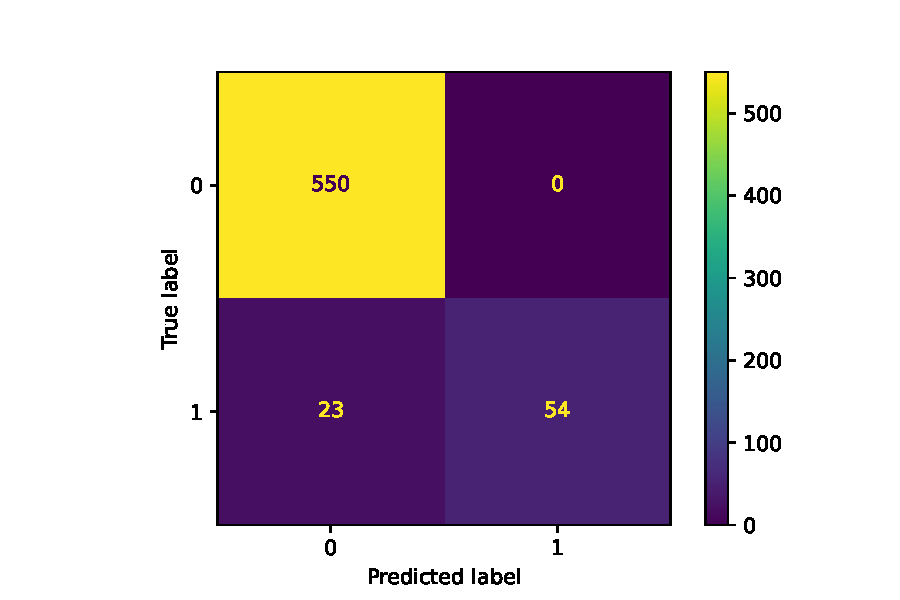
\includegraphics[width=0.7\linewidth]{immagini/mirna_ConfusionMatrixTotalExample}
		\caption{Esempio reale di matrice di confusione calcolata durante gli esperimenti. In particolare, la figura mostra la matrice con la prestazione di AUPRC migliore. È possibile vedere che, per quanto riguarda i pazienti negativi (etichetta 0), il classificatore non sbaglia mai, mentre per quanto riguarda i malati (etichetta 1), il classificatore sbaglia 23 volte su 77. Classifica quindi come sane 23 persone che in realtà sono malate.}
		\label{fig:mirnaconfusionmatrixtotalexample}
	\end{figure}
		
	Esistono diversi algoritmi di apprendimento supervisionato, ognuno dei quali possiede delle caratteristiche peculiari. Di seguito sono stati approfonditi: \textit{Random Forest}, poiché è l'algoritmo usato durante gli addestramenti, e \textit{Decision Tree}, poiché i primi non sono altro che una foresta dei secondi.
	
	\subsubsection{Decision Tree}
	\label{DecisionTree}
	I \textit{Decision Tree}, o alberi di decisione in italiano, sono algoritmi non parametrici\footnote{Categoria di algoritmi di \textit{machine learning} che non richiedono la specificazione di un numero fisso di parametri.} di \textit{supervised learning}. Possono essere utilizzati sia per risolvere problemi di regressione che di classificazione; in particolare in quest'ultima trova maggiore applicazione pratica \cite{Kingsford2008}. Un \textit{Decision Tree} possiede una struttura ad albero, visibile in Figura \ref{fig:DecisionTree} ed è composta da:
	\begin{itemize}
		\item nodi non terminali: rappresentano un test su una o più caratteristiche,
		\item ramo: rappresenta un esito del test,
		\item foglia: rappresenta una possibile classe.
	\end{itemize}
	
	\begin{figure}[h!]
		\centering
		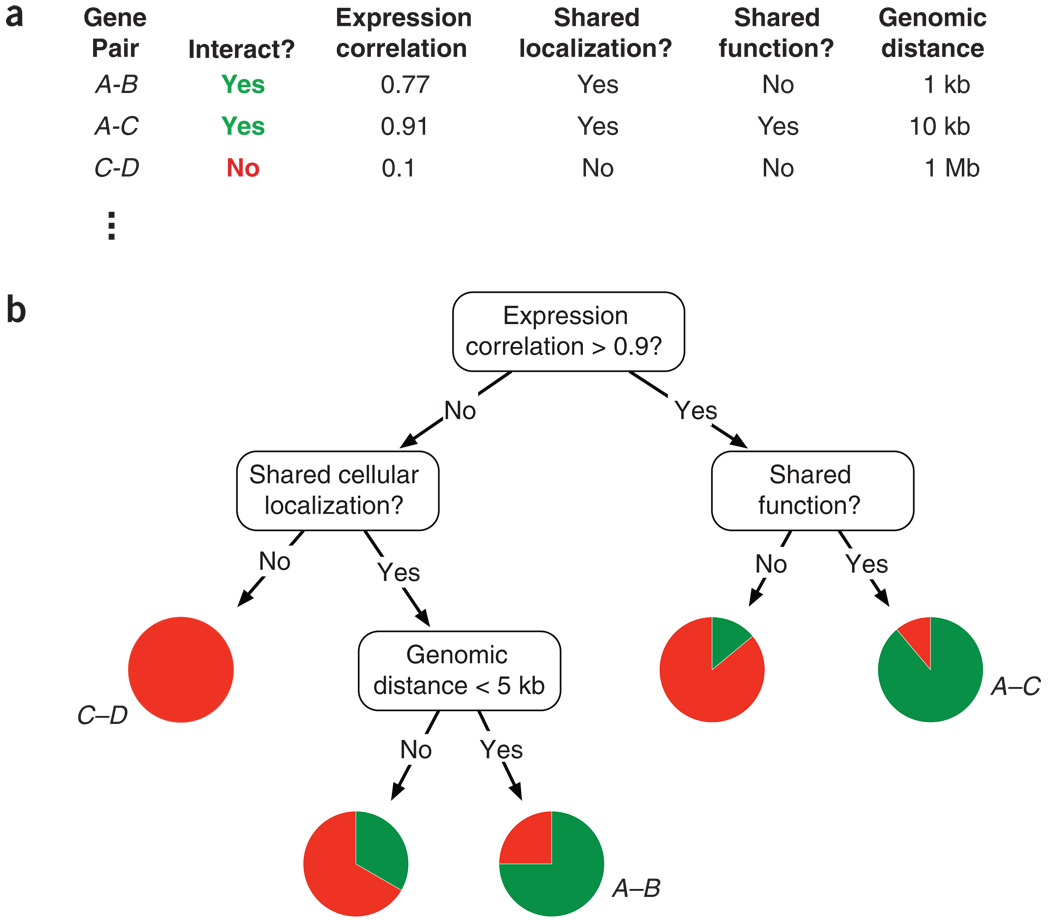
\includegraphics[width=0.7\linewidth]{immagini/DecisionTreeExample2.jpg}
		\caption{a) Ogni dato è una coppia di geni associata a una serie di caratteristiche. Alcune caratteristiche sono numeri a valore reale (\textit{genomic distance} e \textit{expression correlation}), altre sono categoriche (\textit{shared-localization}). (b) Un ipotetico \textit{Decision Tree} in cui ogni nodo contiene una domanda sì/no che riguarda una singola caratteristica dei dati. Un dato naviga l'albero arrivando a una foglia in base alle risposte alle domande. I grafici a torta indicano la percentuale di interagenti (verde) e non interagenti (rosso) degli esempi di addestramento che raggiungono ciascuna foglia. Si prevede che i nuovi esempi interagiscano se raggiungono una foglia prevalentemente verde o non interagiscano se raggiungono una foglia prevalentemente rossa. (fonte: \cite{kingsford2008decision}).}
		\label{fig:DecisionTree}
	\end{figure}
	La costruzione di un \textit{Decision Tree} inizia con la scelta della caratteristica più informativa che viene posta come radice dell'albero. Successivamente vengono identificate le sotto-caratteristiche più informative e vengono utilizzate per creare i nodi figli della radice facendo così una suddivisione. La costruzione dell'albero continua su ogni ramo creando ulteriori nodi figli per ogni nuova sotto-caratteristica identificata. La costruzione dell'albero si arresta quando viene raggiunta una delle condizioni di stop:
	\begin{itemize}
		\item tutti i campioni dei nodi terminali appartengono a una stessa classe,
		\item non ci sono più attributi per un'ulteriore suddivisione.
	\end{itemize}
	Per scegliere la caratteristica su cui effettuare una suddivisione vengono comunemente utilizzati due criteri: la \textit{Gini impurity} e l'entropia.
	
	\paragraph{Gini Impurity}
	La \textit{Gini Impurity} misura la probabilità che un elemento scelto a caso, appartenente a una data classe, sia etichettato in modo errato. Un valore basso indica una maggiore purezza delle classi risultanti dalla suddivisione. Consideriamo un dataset $D$ che contiene
	campioni di $k$ classi diverse. La probabilità che i campioni appartengano alla classe $i$ in un determinato nodo può essere indicata con $p_i$. La \textit{Gini Impurity} di $D$ può essere definita come:
	\begin{equation}
		\text{Gini}(D) = 1- \sum_{k}^{i=1} p_{i}^2.
	\end{equation}
	Il nodo che ha distribuzione di classe uniforme ha l'impurità risultante maggiore. L'impurità minima si ottiene quando tutti i dati appartengono alla stessa classe, quindi l'attributo che genera la minima \textit{Gini Impurity} viene selezionato per dividere il nodo. Se un insieme di dati $D$ viene diviso su un attributo $A$ in due sottoinsiemi $D_1$ e $D_2$ con dimensione, rispettivamente, $n_1$ e $n_2$, la \textit{Gini Impurity} può essere definita come:
	\begin{equation}
		Gini_A(D) = \frac{n_1}{n_2}Gini(D_1) + \frac{n_2}{n}Gini(D_2).
	\end{equation}
	Nel momento in cui si vuole creare un \textit{decision tree} l'attributo che fornisce la minore \textit{Gini Impurity} ($Gini_A(D)$) viene scelto per suddividere l'albero. 
	
	\paragraph{Entropia}
	L'entropia è una misura dell'incertezza associata alle classi. Anche in questo caso, un valore basso indica una maggiore purezza delle classi risultanti dalla suddivisione, più è alta, più l'insieme dei dati è eterogeneo. La formula per calcolare l'entropia è la seguente:
	\begin{equation}
		Entropia = -\sum (p_i * log_2(p_i)),
	\end{equation}
	dove $p_i$ è la probabilità che un dato appartenga alla classe $i$, la somma viene fatta su tutte le classi presenti nell'insieme di dati. L'entropia è zero quando tutti gli esempi appartengono alla stessa classe e massima quando tutte le classi sono ugualmente rappresentate. 
	
	Il criterio di scelta può essere utilizzato per valutare tutti gli attributi disponibili e scegliere quello che produce la suddivisione con il valore più basso.
	In generale si usano questi criteri per evitare \textit{overfitting} (vedi Paragrafo \ref{Overfitting}) e aiutare a generalizzare meglio il modello su dati sconosciuti.
	Queste tecniche sono euristiche e riescono a trovare un albero efficiente che però non corrisponde necessariamente all'ottimo. La ricerca dell'albero ottimale è computazionalmente difficile perché il numero di possibili alberi cresce molto rapidamente con il numero di attributi. Prendiamo, per esempio, un insieme di dati con un numero di attributi pari a $n$ che ha solo due valori possibili per ogni attributo, ci sono così $2^n$ possibili alberi di decisione. Se invece ci fossero stati $m$ valori possibili per ogni attributo, allora ci sarebbero stati al massimo $m^n$ possibili alberi di decisione.
	
	La ricerca dell'albero ottimo necessiterebbe quindi dell'esplorazione di tutte queste possibilità e successivamente della valutazione di quale sia l'albero che ha il minor errore sui dati di addestramento. Per questo motivo vengono usati algoritmi \textit{greedy} che creano l'albero prendendo decisioni localmente ottime usando la \textit{Giny Impurity} o l'entropia.


	\subsubsection{Random Forest}
	\label{RandomForest}
	Un \textit{Random Forest}, o foresta aleatoria in italiano, proposto da L. Breiman nel 2001 \cite{Breiman2001}, è un modello matematico di tipo \textit{ensamble}\footnote{L'\textit{ensamble} è una tecnica di \textit{Machine Learning} che combina più modelli per ottenere una \textit{performance} migliore rispetto a quella ottenuta da ogni modello singolo. Ciò avviene creando diversi modelli di base (ad esempio, \textit{Decision Tree} o reti neurali) su sottoinsiemi differenti dei dati di addestramento e quindi combinando le loro previsioni in una previsione finale.} che utilizza un insieme di \textit{Decision Tree}, illustrati nel paragrafo precedente, per fare previsioni. Ciascun \textit{Decision Tree} viene allenato su un sottoinsieme casuale di dati di addestramento e le previsioni finali sono ottenute tramite una votazione di maggioranza o come media delle previsioni degli alberi. 
	
	Un modello di questo tipo risulta più robusto e con una precisione migliore rispetto all'utilizzo di un singolo \textit{Decision Tree}. Esistono diversi motivi per cui si preferisce usare \textit{Random Forest} piuttosto che un singolo \textit{Decision Tree}:
	\begin{itemize}
		\item miglioramento della precisione: usando più \textit{Decision Tree} di solito la precisione finale del modello aumenta,
		\item riduzione dell'\textit{overfitting}: i singoli \textit{Decision Tree} possono soffrire di \textit{overfitting}. \textit{Random Forest} utilizza allora una serie di \textit{decision tree} e prende la decisione finale come voto di maggioranza. Si può dimostrare che ciò riduce l'effetto dell'\textit{overfitting},
		\item rilevamento di \textit{feature} importanti: \textit{Random Forest} permette di individuare quali sono le \textit{feature} più importanti per classificare i dati,
		\item scalabiltà: \textit{Random Forest} scala molto bene con \textit{dataset} grandi.
	\end{itemize}
	È anche possibile usare un \textit{random forest} per fare regressione. In questo caso il \textit{Random Forest} si forma facendo crescere il numero di \textit{Decision Tree} in funzione di un vettore casuale in modo che il predittore assuma valori numerici anziché etichette di classe. I valori di \textit{output} sono numerici e si assume che il \textit{training set} sia estratto in modo indipendente dalla distribuzione del vettore casuale \cite{Breiman2001}.
	
	Questo modello presenta diversi iperparametri i cui valori vengono utilizzati per controllare il processo di apprendimento e di conseguenza le prestazioni del modello rispetto ai dati. Essi sono parametri che non vengono impostati automaticamente dal modello durante l'addestramento ma vengono stabiliti a priori. Tra i più noti troviamo:
	\begin{itemize}
		\item \textit{n\_estimators}: numero di alberi nella foresta,
		\item \textit{max\_depth}: profondità massima degli alberi,
		\item \textit{min\_samples\_split}: numero minimo di campioni richiesto per dividere un nodo,
		\item \textit{min\_samples\_leaf}: numero minimo di campioni richiesto in una foglia,
		\item \textit{max\_features}: numero massimo di caratteristiche considerate per la divisione in ogni nodo,
		\item \textit{criterion}: funzione per misurare la qualità di una divisione. Alcuni esempi sono: \textit{Gini impurity} ed entropia.
	\end{itemize} 
		Questi iperparametri possono essere regolati per migliorare le prestazioni del modello e prevenire l'\textit{overfitting}. La scelta ottimale degli iperparametri può essere effettuata utilizzando tecniche di \textit{tuning} (vedi Paragrafo \ref{tuning}).
	
	\subsection{Unsupervised Learning}
	Nel \textit{Unsupervised Learning}, anche chiamato apprendimento non supervisionato in italiano, si ha un insieme di dati $X$ (\{$x_1, x_2,...,x_n$\}) ma in questo caso non sono presenti né un'etichetta, come invece c'è nel \textit{Supervised Learning} (vedi Paragrafo  \ref{SupervisedLearning}), né ricompense dall'ambiente, come invece accade nel \textit{Reinforced Learning} (vedi Paragrafo \ref{reinforcedLearning}). Può sembrare un po' misterioso immaginare cosa possa riuscire a estrapolare il sistema dai dati senza alcun \textit{feedback} dato dall'etichetta o dall'ambiente. Tuttavia, è possibile sviluppare un \textit{framework}\footnote{Il framework è un insieme di regole, linee guida e metodologie che forniscono una struttura per la costruzione di un sistema, un prodotto o un processo. In informatica, un \textit{framework} può essere utilizzato per creare software, sviluppare applicazioni o semplificare lo sviluppo di soluzioni.} per fare \textit{Unsupervised Learning} nel quale l'obiettivo è quello di costruire rappresentazioni dell'\textit{input} in modo che possano risultare utili per prendere decisioni, prevedere \textit{input} futuri e in generale ricercare modelli il più possibile esenti da rumore \cite{Ghahramani2004}.
	Due esempi classici di \textit{Unsupervised Learning} sono il \textit{clustering} e la riduzione della dimensionalità.
	Il \textit{clustering} è una tecnica che consiste nel raggruppare un insieme di oggetti in modo che quelli dello stesso gruppo (\textit{cluster}) siano più simili (rispetto a una determinata proprietà) tra loro rispetto a quelli di altri \textit{cluster}. In generale esistono molte tecniche per fare \textit{clustering} e la scelta dipende dalle applicazioni e dalle proprietà dei dati. Una delle tecniche di \textit{clustering} più utilizzata è senza dubbio \textit{K-means} \cite{morissette2013k}.
	I dati del mondo reale hanno solitamente un'elevata dimensionalità, è necessario quindi ridurne la dimensionalità per riuscire a gestirli in maniera adeguata. La riduzione della dimensionalità è una tecnica di trasformazione dei dati ad alta dimensionalità in una rappresentazione a dimensione ridotta. Questa pratica è importante in molti ambiti, poiché attenua la \textit{curse of dimensionality}\footnote{Il \textit{curse of dimensionality}, la maledizione della dimensionalità in italiano, è un termine introdotto da Bellman per descrivere il problema causato dall'aumento esponenziale del volume associato all'aggiunta di ulteriori dimensioni allo spazio euclideo \cite{Keogh2017}.} e altre proprietà indesiderate degli spazi ad alta dimensionalità \cite{Jimenez1998SupervisedCI}.

	
	\subsection{Semi-Supervised Learning}
	Il \textit{Semi-Supervised Learning}, anche chiamato apprendimento semi-supervisionato in italiano, è un tipo di \textit{machine learning} in cui dei dati che vengono passati all'algoritmo solamente una piccola parte è etichettata. L'obiettivo è quello di usare i dati etichettati per riuscire a fornire un'etichetta automaticamente anche ai dati che ne sono privi. Esistono diverse tecniche per fare questo, come ad esempio le tecniche di propagazione delle etichette \cite{LearningfromLabeledandUnlabeledDatawithLabelPropagation}, le tecniche di \textit{co-training} \cite{10.1145/279943.279962}, le tecniche di \textit{self-training} \cite{inproceedings}.
	
	
	\subsection{Reinforced Learning}
	\label{reinforcedLearning}
	Nel \textit{Reinforced Learning}, anche chiamato apprendimento per rinforzo in italiano, un agente è connesso all'ambiente tramite percezione e azione, come visibile in Figura \ref{fig:reinforcedlearningmodel}. A ogni step di interazione, l'agente riceve in ingresso, $i$, un'indicazione dello stato corrente, $s$, dell'ambiente; quindi l'agente sceglie un'azione, $a$, per generare un \textit{output}. L'azione cambia lo stato dell'ambiente e il valore di questa transizione di stato viene comunicato all'agente attraverso un segnale di rinforzo, $r$. Il comportamento dell'agente, $B$, dovrebbe scegliere azioni che tendono a massimizzare il segnale di rinforzo. Di seguito vengono elencate le diverse fasi dell'apprendimento per rinforzo.
	\begin{itemize}
		\item L'agente inizialmente agisce in maniera casuale, non avendo nessuna conoscenza dell'ambiente;
		\item interagendo con l'ambiente l'agente inizia a prendere decisioni e ottenere così le ricompense;
		\item ottenendo le ricompense l'agente ``capisce'' come deve agire e adatta la sua \textit{policy} con l'obiettivo di massimizzare la ricompensa.
	\end{itemize}
	
	\begin{figure}[h]
		\centering
		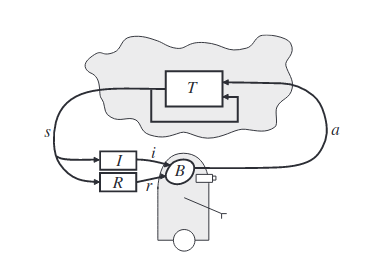
\includegraphics[width=0.7\linewidth]{immagini/ReinforcedLearningModel}
		\caption{Modello standard di \textit{reinforced learning} (fonte: \cite{kaelbling1996reinforcement}.)}
		\label{fig:reinforcedlearningmodel}
	\end{figure}
	
	
	\subsection{Machine Learning in Bioinformatica}
	L'apprendimento automatico viene utilizzato in tantissimi ambiti di ricerca \cite{Sarker2021}: analisi predittiva e processo decisionale intelligente, sicurezza informatica, \textit{internet of things} e città \textit{smart}, previsione del traffico, trasporto pubblico, \textit{healthcare}, pandemia dovuta al COVID-19, NLP ecc.
	Questa tecnologia trova spazio anche all'interno della bioinformatica, ovvero l'applicazione di tecniche di calcolo per acquisire e interpretare i dati biologici. È un campo interdisciplinare tra informatica, matematica, statistica, biologia e genetica. 	
	La crescita esponenziale di dati biologici disponibili ha sollevato due problemi: trovare un modo efficiente per immagazzinare e gestire dati di questo tipo e riuscire a sfruttarli per arrivare a estrarre informazioni utili. I domini in cui vengono utilizzate tecniche di \textit{machine learning} sono molte: in Figura \ref{fig:utilizzimachinelearningbioinfo} vengono mostrati sei diversi domini nei quali si utilizzano metodi computazionali in ambito bioinformatico: genomica, proteomica, microarray, biologia dei sistemi, evoluzione e \textit{text mining}.
	
	\begin{figure}[h]
		\centering
		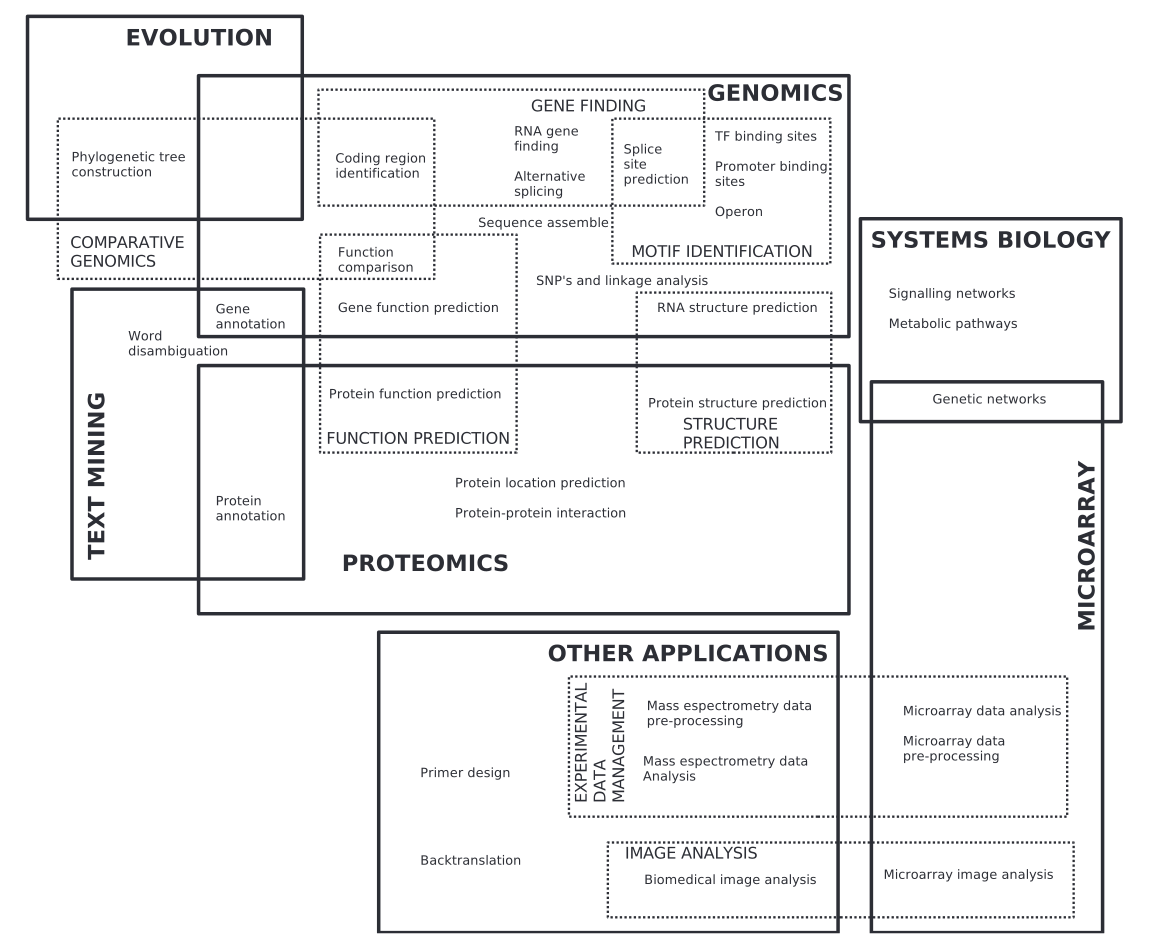
\includegraphics[width=1\linewidth]{immagini/utilizziMachineLearningBioinfo}
		\caption[]{Classificazione dei campi in cui vengono applicati metodi di apprendimento automatico in bioinformatica (fonte: \cite{Machine_Learning_in_Bioinformatics}).}
		\label{fig:utilizzimachinelearningbioinfo}
	\end{figure}

	La genomica è una delle aree più importanti in bioinformatica. Il numero di sequenze nucleotidiche e proteiche disponibili è in continuo aumento. In Figura \ref{fig:growthofgenbank} è possibile vedere la crescita di dati disponibili dal 1982 al 2020. GenBank è una banca dati a libero accesso e senza restrizione, istituita nel 1982, che riporta tutte le sequenze di nucleotidi e le relative proteine ottenute dopo la loro traduzione. GenBank riceve le proprie informazioni dai risultati ottenuti su oltre 300.000 organismi da laboratori distinti sparsi in tutto il mondo, rappresentando il più importante punto di riferimento nel relativo campo di ricerca. A febbraio 2020, conteneva oltre 216 milioni di loci\footnote{In genetica, il termine \textit{locus} genico (o più semplicemente \textit{locus}, plurale \textit{loci}) designa la posizione, stabile, di un gene o di un marcatore genico all'interno di un cromosoma.} e oltre 399 miliardi di basi da più di 216 milioni di sequenze riportate.

	\begin{figure}[h]
		\centering
		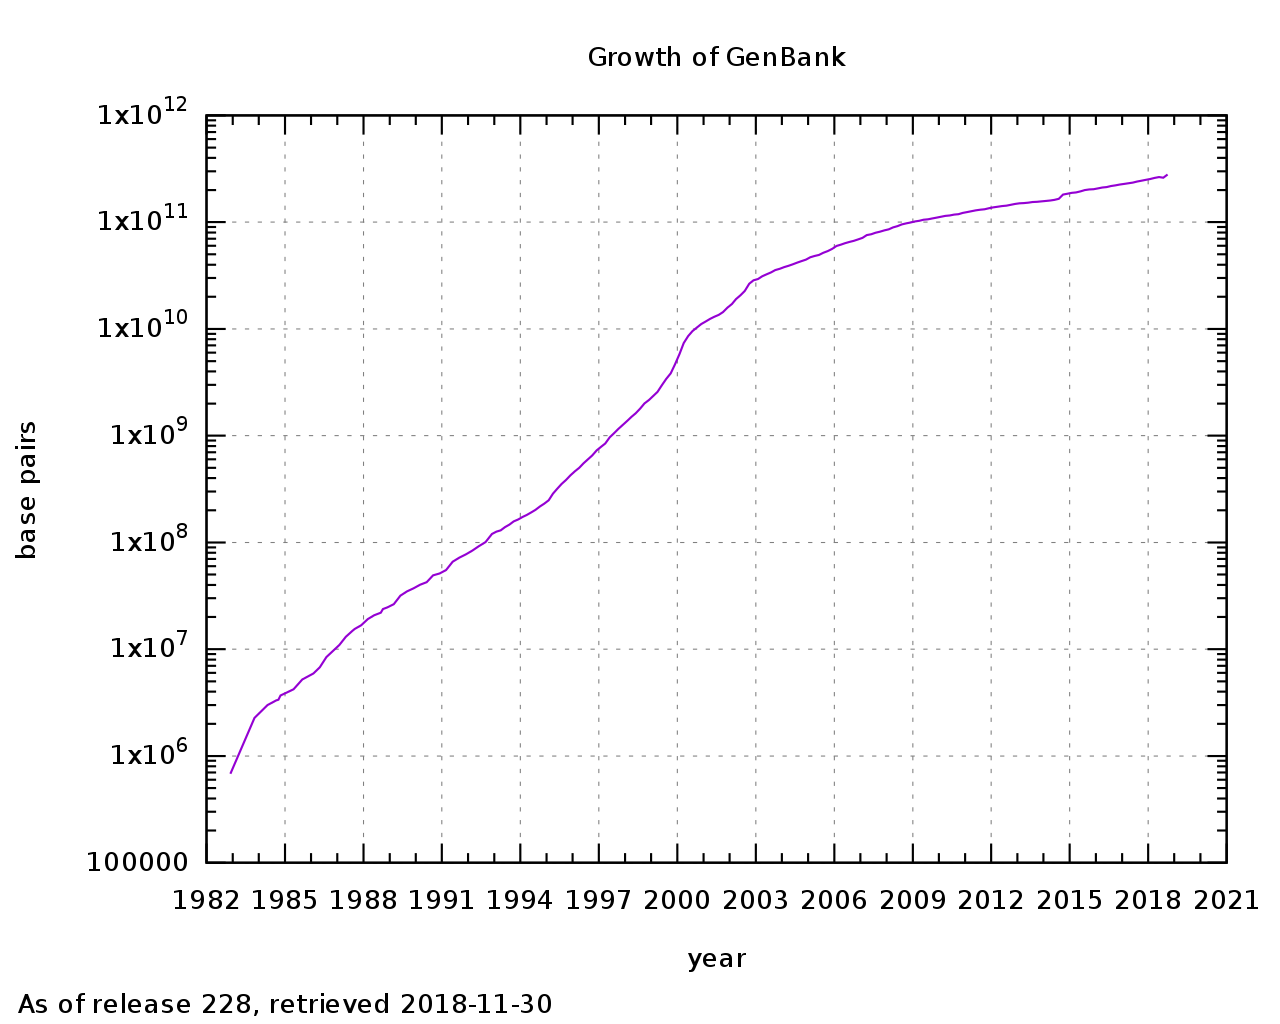
\includegraphics[width=0.8\linewidth]{immagini/Growth_of_Genbank.svg}
		\caption{Crescita di GenBank (fonte: \cite{geneBANK}).}
		\label{fig:growthofgenbank}
	\end{figure}
	Tutti questi dati hanno bisogno di essere elaborati in modo da estrapolare informazioni utili. Come prima cosa  è possibile estrarre struttura e posizione dei geni dalle sequenze del genoma \cite{Mathe2002-us}, inoltre è anche possibile identificare gli elementi regolari \cite{Aerts2004-jh}. Esistono inoltre approcci per estrarre caratteristiche comuni tra gli RNA noti per la previsione di nuovi geni RNA nelle regioni non annotate dai genomi procariotici e arcaici \cite{Carter2001-oo}.
	
	Nella proteomica i metodi computazionali vengono usati per la previsione della struttura delle proteine. Le proteine hanno una struttura molto complessa composta da migliaia di atomi e legami, di conseguenza il numero di possibili strutture è estremamente elevato. La previsione della struttura risulta quindi un problema combinatorio molto complesso e richiede una buona ottimizzazione.
	
	Attraverso l'applicazione dei metodi computazionali è possibile anche gestire dati sperimentali complessi. Il campo più noto dove troviamo applicazioni di questo tipo sono i \textit{microarray}\footnote{Un \textit{microarray} è una piastra di vetro o policarbonato che contiene migliaia di probe, ovvero sequenze di DNA, genetiche fissate sulla sua superficie, utilizzata per monitorare l'espressione genica su larga scala.}. Possono essere utilizzati, ad esempio, per la classificazione di tumori, la previsione della risposta ai farmaci, la scoperta di nuovi geni e biomarcatori. Inoltre i \textit{microarray} possono anche essere utilizzati per l'analisi dell'espressione genica durante lo sviluppo, lo stress o la risposta ai trattamenti farmacologici \cite{butte2002use}.
	  
	Nei paragrafi che seguono sono stati discussi alcuni esempi pratici di applicazione di tecniche di apprendimento automatico in campo bioinformatico e medico.
	
	\subsection{Apprendimento automatico per la previsione di varianti non codificanti associate a malattie}
	All'interno di tutte le variazioni genetiche, quelle riguardanti le malattie rappresentano una piccolissima minoranza rispetto all'insieme più ampio di variazioni genomiche non deleterie. Questo comporta uno sbilanciamento tra i sottoinsiemi che compongono le variazioni genomiche. Quello che si vorrebbe fare è usare tecniche di \textit{machine learning} per individuare varianti non codificanti associate alle malattie, ma la scarsità di osservazioni inficia l'efficacia delle tecniche. Lo stato dell'arte dei metodi basati sul \textit{machine learning} non adotta tecniche specifiche che tengano conto dello sbilanciamento dei dati e questo porta inevitabilmente a una riduzione della sensibilità e della precisione nei risultati.
	
	In questo contesto gli algoritmi di apprendimento classici come quelli collegati a \textit{support vector machine} \cite{Cortes1995} o \textit{artificial neural networks} \cite{bishop1995neural} non riescono a generalizzare in maniera sufficiente poiché di solito prevedono la classe di minoranza con una precisione e sensibilità molto bassa.
	Nel campo della previsione di varianti genetiche associate a tratti o malattie, questo si riduce a prevedere erroneamente la maggior parte delle varianti associate alla malattia come non associate alla malattia stessa. Viene così limitata in modo significativa l'utilità dei metodi di apprendimento supervisionato per la previsione di nuove varianti non codificanti.
	
	Per affrontare questo problema è stato sviluppato \textit{hyper}SMURF \cite{Schubach2017} sigla che sta a indicare: \textit{hyper-ensemble of SMOTE Undersampled Random Forest}. Questo metodo adotta strategie di apprendimento che tengono conto dello sbilanciamento, ovvero tecniche di ricampionamento e su un approccio \textit{hyper-ensemble}: simultaneamente la classe di minoranza viene sovracampionata e la classe di maggioranza viene sottocampionata in modo da generare dati di addestramento bilanciati, ciascuno dei quali verrà poi usato per addestrare un insieme di \textit{Random Forest}. La sua struttura è visibile in Figura \ref{fig:hypersmurf}.
	\begin{figure}[h!]
		\centering
		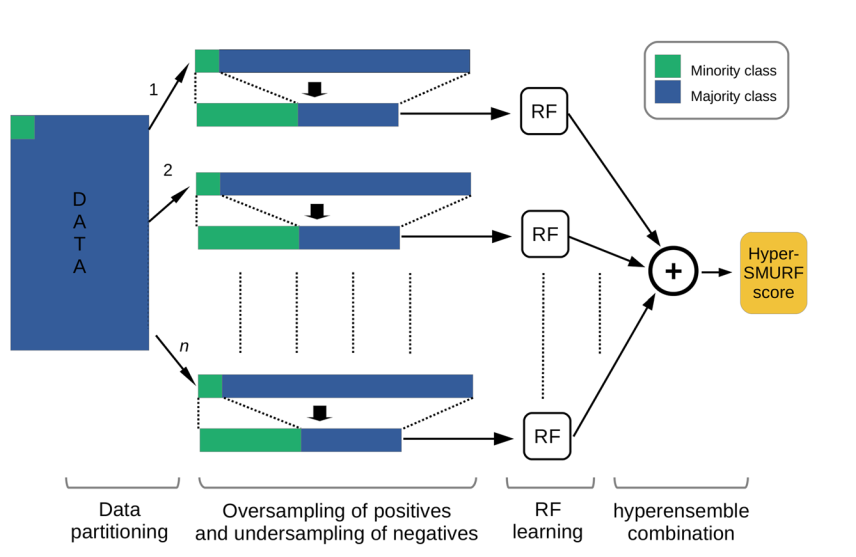
\includegraphics[width=0.7\linewidth]{immagini/hyperSMURF}
		\caption{Schema di \textit{hyper}SMURF. Esso divide la classe maggioritaria (rettangoli blu) in $n$ partizioni e per ognuna di esse vengono usate tecniche di sovracampionamento in modo da generare esempi aggiuntivi dalla classe minoritaria (rettangoli verdi). Contemporaneamente un numero simile di esempi viene sottocampionato dalla classe maggioritaria. Successivamente \textit{hyper}SMURF addestra in parallelo $n$ \textit{Random Forest} usando i dati bilanciati e infine combina le predizioni degli $n$ insiemi secondo un approccio \textit{hyper-ensemble} (fonte: \cite{Schubach2017}).}.
		\label{fig:hypersmurf}
	\end{figure}

	Successivamente le predizioni dei modelli addestrati sono combinate attraverso un approccio chiamato \textit{hyper-ensemble} per ottenere una predizione complessiva ``concordata''. Vengono addestrati, in parallelo, $n$ \textit{Random Forest}, una per ogni insieme di dati, e vengono combinate le loro previsioni facendo la media delle probabilità, si ottiene un \textit{hyper-ensemble} poiché l'\textit{input} è a sua volta un insieme di \textit{decision tree}. 
	
	Il vantaggio risiede nel fatto di avere molta diversità nei dati di addestramento, inoltre il bilanciamento tra esempi positivi e negativi evita che si abbia una polarizzazione verso la classe maggioritaria. Tutto ciò rende il modello maggiormente in grado di generalizzare, mentre l'approccio di \textit{hyper-ensemble} fornisce apprendimento più accurato e previsioni più robuste.
	Per testare il modello viene utilizzata una $10$-\textit{cross-validation} per assicurarsi che le varianti della stessa malattia non si presentino insieme nel \textit{training set}, o insieme di addestramento, e in quello di \textit{test}, falsando così i risultati. La misura vera e propria è affidata all'AUPRC, ovvero \textit{Area Under the Precision and Recall}, all'AUROC, \textit{Area Under the Receiver Operating Characteristic} e usando la \textit{precision}, \textit{recall} e \textit{F-score}, discussi in Paragrafo \ref{SupervisedLearning}.
	
	\begin{figure}[h]
		\centering
		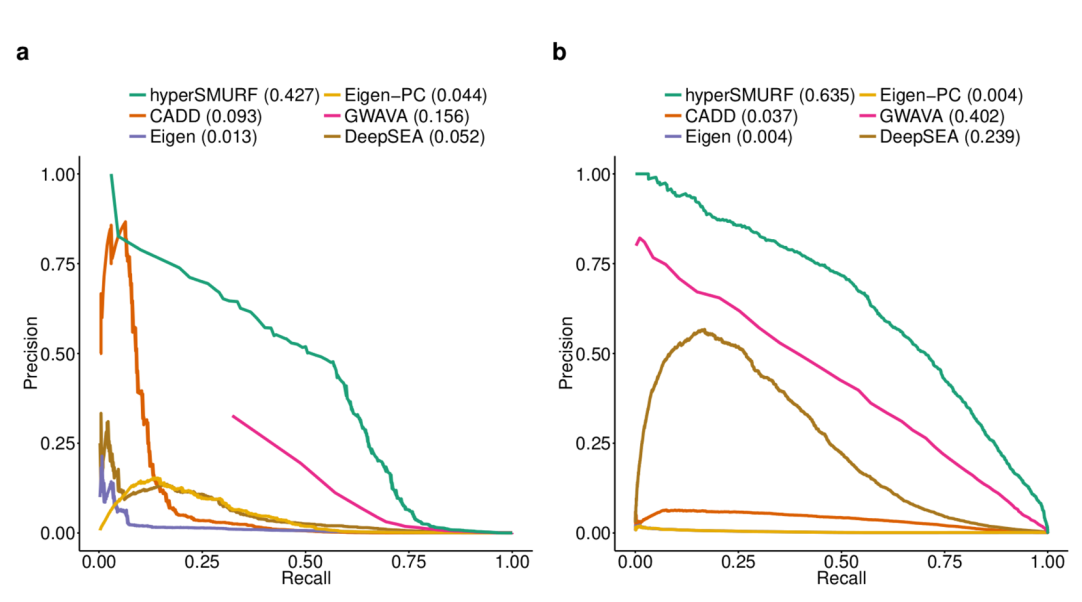
\includegraphics[width=0.8\linewidth]{immagini/ResultHyperSMURF}
		\caption{Confronto della curva \textit{precision/recall} tra i vari modelli usando due tipi diversi di dati: a) \textit{Mandelian regulatory mutations}, b) \textit{GWAS regulatory hits}. Il numero tra parentesi rappresenta il valore di AUPRC (fonte: \cite{Schubach2017}).}
		\label{fig:resulthypersmurf}
	\end{figure}

	I risultati sono visibili in Figura \ref{fig:resulthypersmurf} dove è possibile trovare un confronto tra i vari metodi usando la curva \textit{precision-recall}. Si nota chiaramente come \textit{hyper}SMURF raggiunga migliori risultati rispetto ai metodi classici.
	
	
	\subsection{Apprendimento automatico per la previsione del rischio di COVID-19}
	Negli ultimi anni una grave sindrome respiratoria (SARS-Cov-2) ha colpito il mondo provocando una pandemia mondiale e causando $663$ milioni di casi accertati e quasi $7$ milioni di morti accertati \cite{covidDeath}. In Figura \ref{fig:COVID_deaths_and_cases} sono illustrati i grafici dei casi totali e morti totali da quando è scoppiata la pandemia.

	\begin{figure}[h!]
		\centering
		\begin{subfigure}[b]{0.85\textwidth}
			\centering
			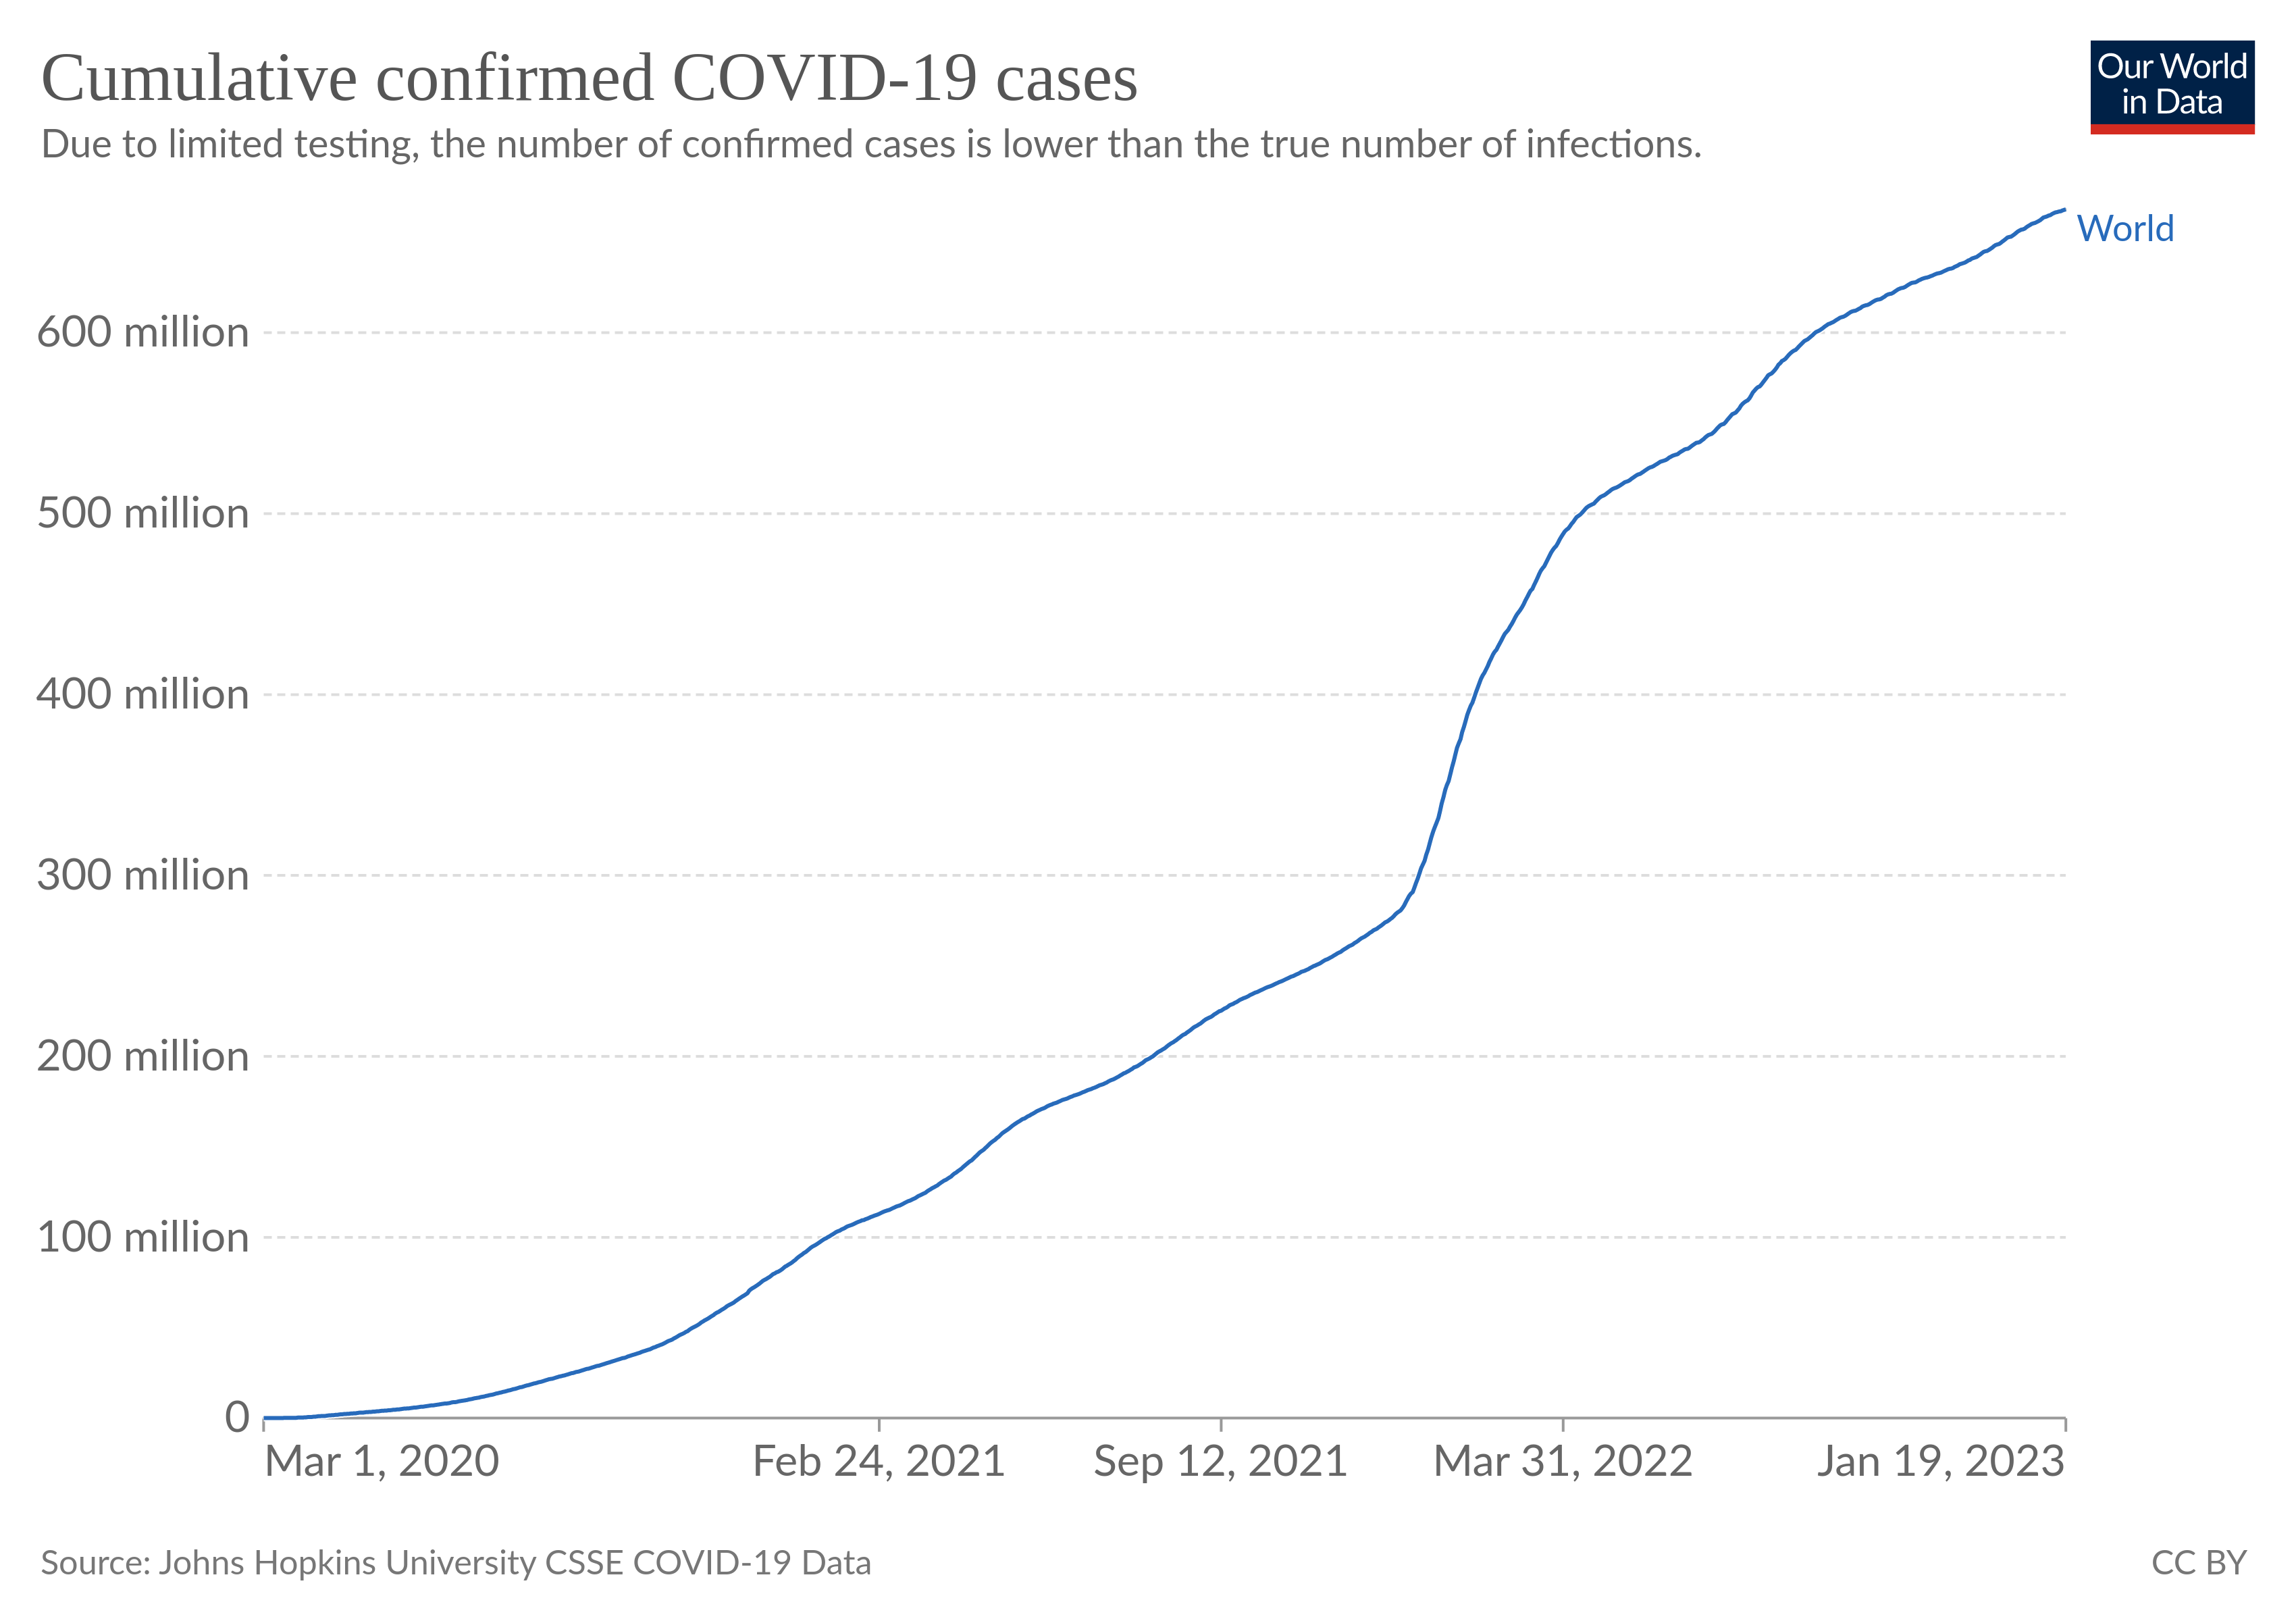
\includegraphics[width=0.90\linewidth]{immagini/coronavirus-data-explorer_cases}
			\caption{}
			\label{fig:coronavirus-data-explorercases}
		\end{subfigure}
		\begin{subfigure}[b]{0.85\textwidth}
			\centering
			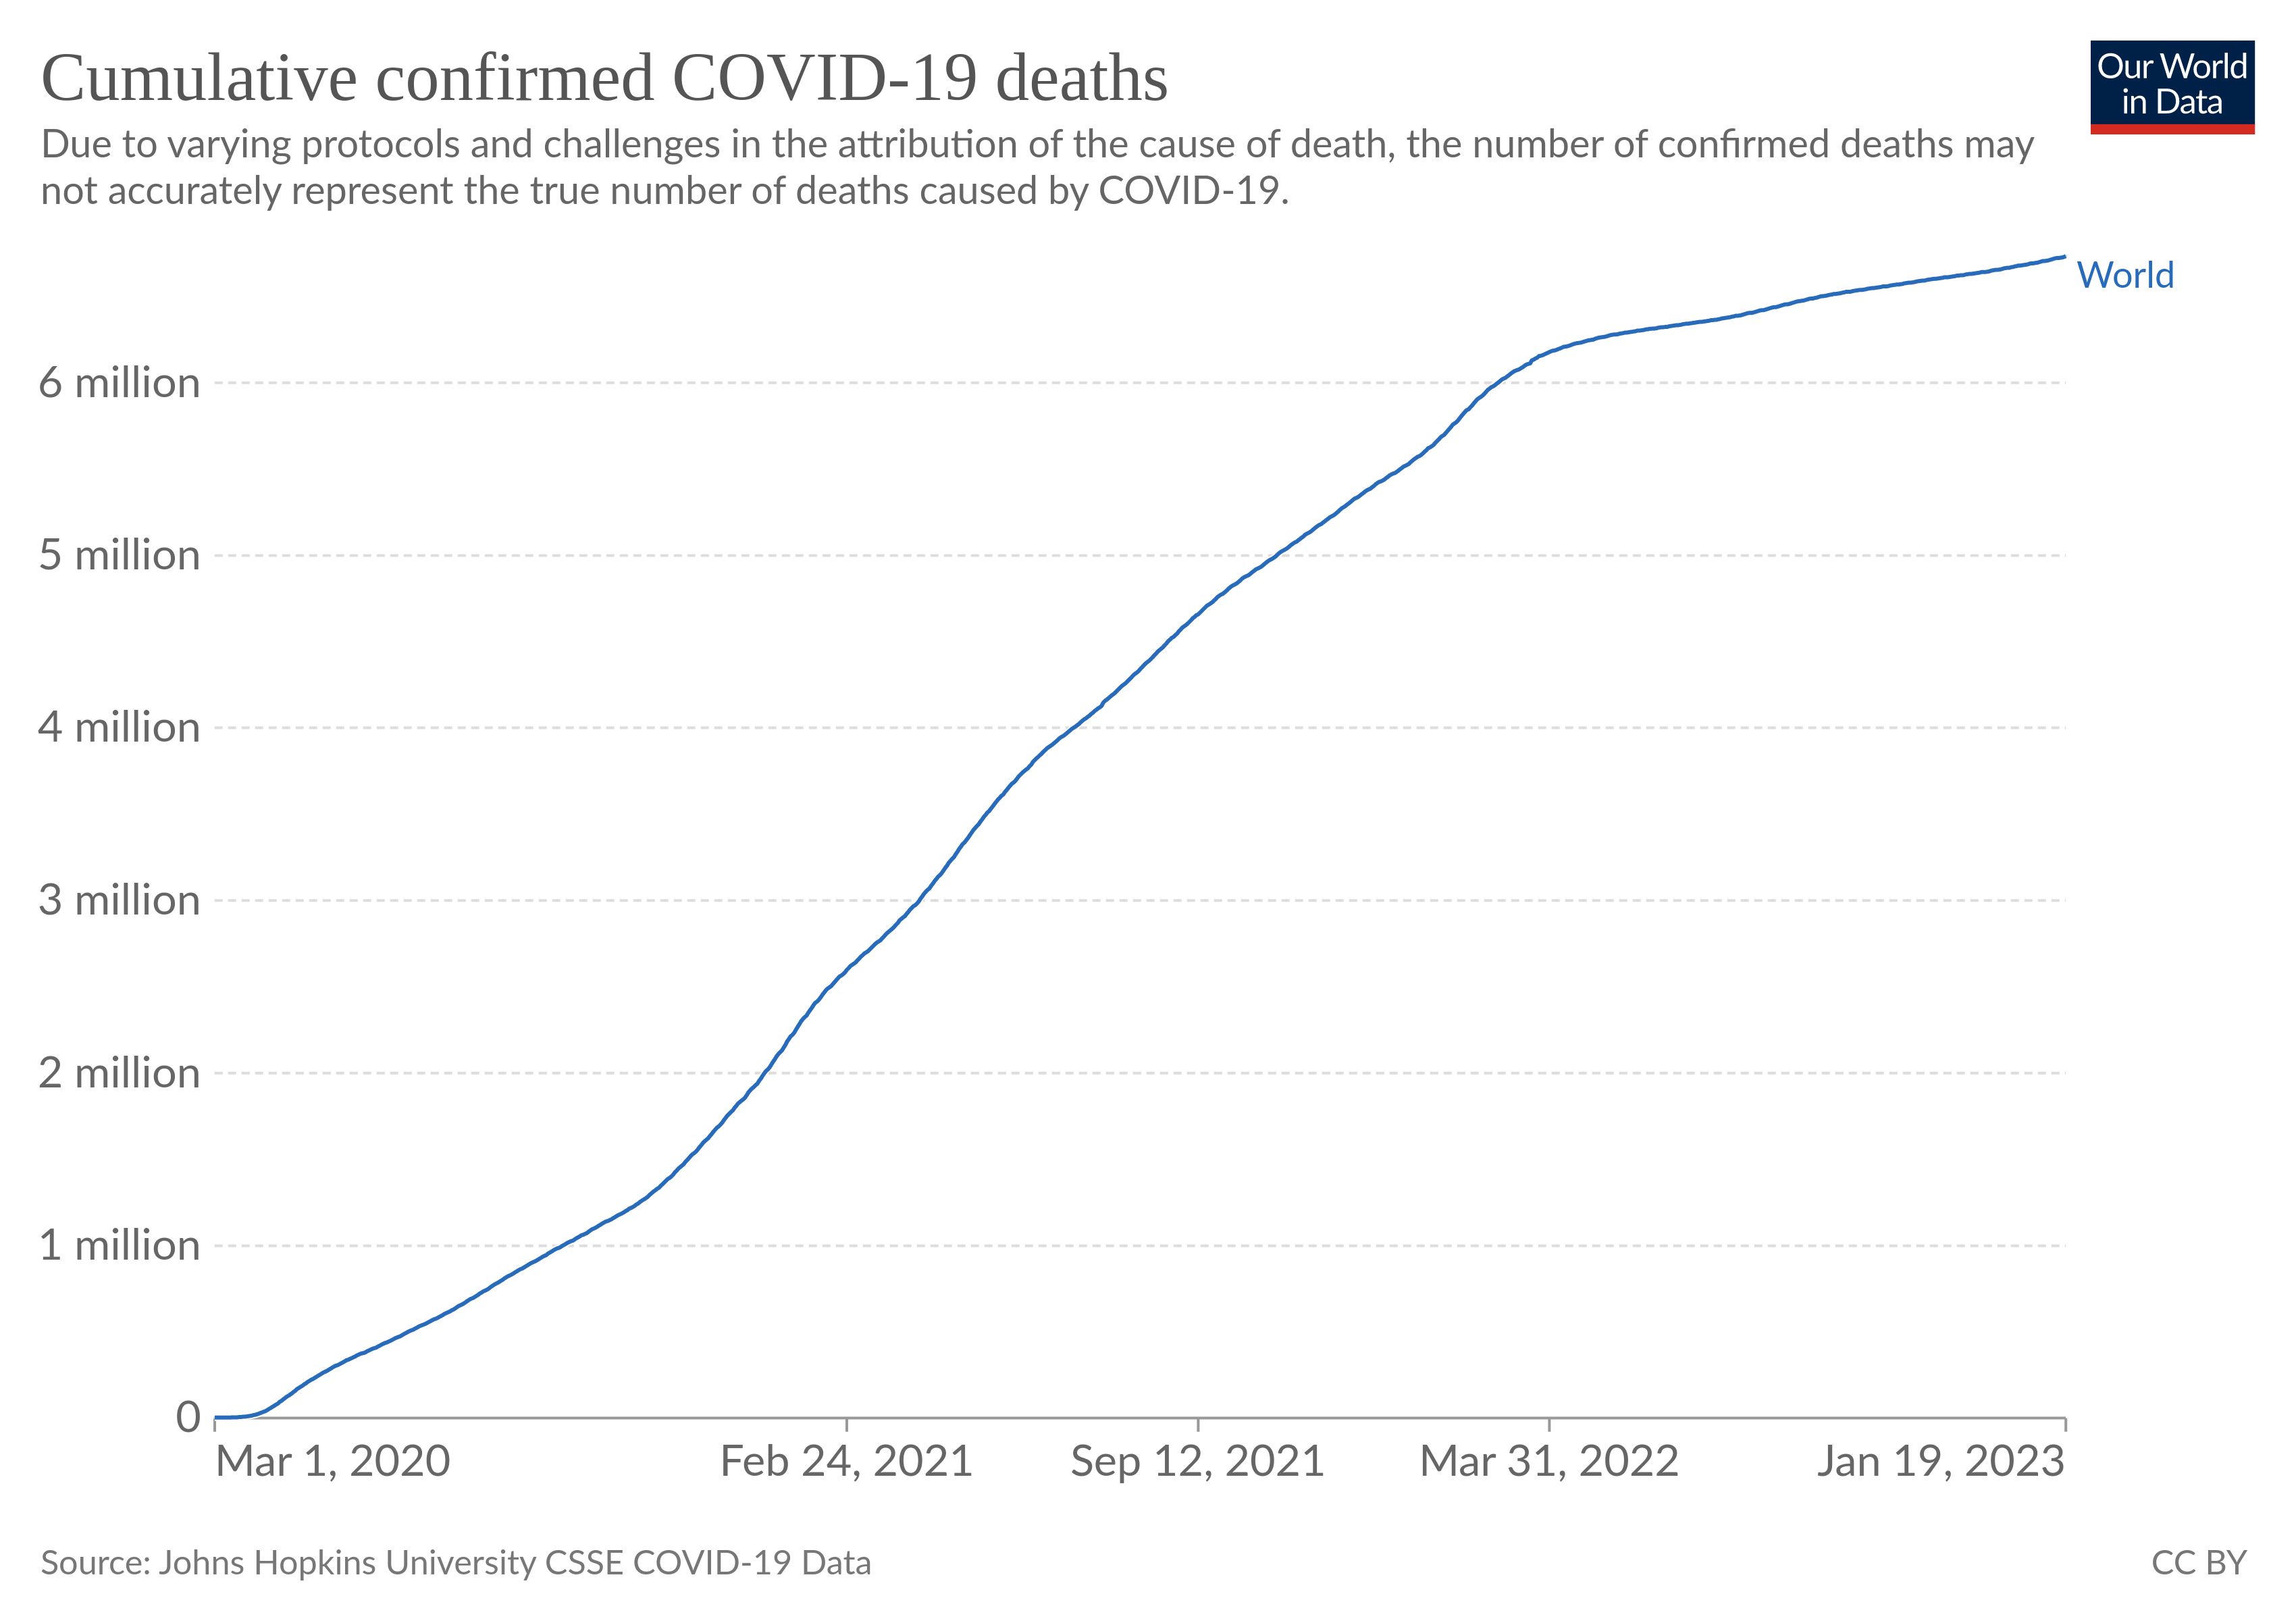
\includegraphics[width=0.90\linewidth]{immagini/coronavirus-data-explorer_death}
			\caption{}
			\label{fig:coronavirus-data-explorerdeath}
		\end{subfigure}
	\caption{Grafico che mostra a) casi totali e b) morti totali nel mondo da quando è scoppiata la pandemia a oggi (fonte \cite{covidExplorer}).}
	\label{fig:COVID_deaths_and_cases}
	\end{figure}

	Da quando il virus ha iniziato a diffondersi tra la popolazione, ospedali e pronto soccorso sono stati invasi da pazienti per i quali era necessario sapere se avessero contratto la malattia o meno ma sopratutto la gravità di quest'ultima. Il virus era ed è in grado di causare anomalie nelle radiografie del torace (CXR)\footnote{\textit{Chest-X-Ray} è un esame radiologico che utilizza la radiazione a raggi X per creare immagini del torace. Questo esame viene spesso utilizzato per diagnosticare o monitorare una serie di condizioni mediche, tra cui malattie polmonari (come la bronchite, l'enfisema o la polmonite), malattie cardiache (come la cardiopatia), tumori e altri problemi che interessano la zona toracica.}. Questo tipo di esame però non basta per determinare la presenza o meno della malattia a causa della sua bassa sensibilità. Il CXR ha però il vantaggio di essere economico e si vuole cercare di sfruttarlo assieme a ulteriori considerazioni e criteri per riuscire a prevedere il rischio di aver contratto il virus con conseguente scoperta della gravità.
	L'obiettivo è quello di riuscire a creare un sistema che riesca a estrarre le variabili radiologiche, cliniche e di laboratorio più rilevanti che siano in grado di migliorare la previsione del rischio del paziente. Si vogliono inoltre ottenere criteri utilizzabili dai medici nel momento in cui devono decidere il rischio del paziente, inteso come gravità della malattia. In \cite{Casiraghi2020-zt} viene illustrato un modello di previsione del rischio per il paziente. Il modello è in grado di selezionare le più importanti variabili cliniche e di laboratorio tenendo anche conto di punteggi radiologici che derivano dalla valutazione del CXR da parte dei radiologi e due punteggi di ``coinvolgimento polmonare'' calcolati usando alcune delle \textit{deep neural network} più performanti per la diagnosi del rischio da COVID-19 \cite{irvin2019chexpert, ma2020survey, bressem2020comparing}, come \textit{ResNet} \cite{he2016deep, narin2021automatic}, \textit{Inception-Net} \cite{szegedy2017inception, das2020truncated} o \textit{VGG} \cite{apostolopoulos2020covid, shibly2020covid}.
	Successivamente viene eseguita una fase di imputazione dei dati mancanti causata dall'integrazione di più fonti di dati. Le tecniche usate sono state la \textit{Multiple Imputations by Chained Equations} (MICE \cite{JSSv045i03}), sia utilizzando la corrispondenza media predittiva (\textit{micePMM} \cite{gaffert2016towards}), sia classificatori \textit{Random Forest} (\textit{miceRF})  come modello di imputazione di \textit{bias}, e \textit{missForest} \cite{10.1093/bioinformatics/btr597}.
	In seguito viene costruito un algoritmo robusto che combina Boruta \cite{JSSv036i11, Kursa2010} con metodi di \textit{feature selection}, basati sulle permutazioni e incorporati nelle \textit{random forest} \cite{Strobl2007}.
	
	Le \textit{feature} selezionate sono usate come \textit{input} per \textit{random forest}, (vedi Paragrafo \ref{RandomForest}) e per alberi associativi derivati \cite{e1bb70540db14ceeacddd4383fca9bff}. A differenza dei \textit{random forest} che producono un gran numero di regole di difficile comprensione, gli alberi associativi derivati sono costruiti partendo dai primi ma producendo regole più semplici che possono essere facilmente valutate e interpretate dai medici.
	I risultati ottenuti dai due algoritmi sono comparati a quelli ottenuti dai modelli generalizzati (GLM \cite{10.2307/2344614}). In Figura \ref{fig:resultcovidmodel} è possibile vedere i punteggi ottenuti con i modelli citati precedentemente.
	
	\begin{figure}[t]
		\centering
		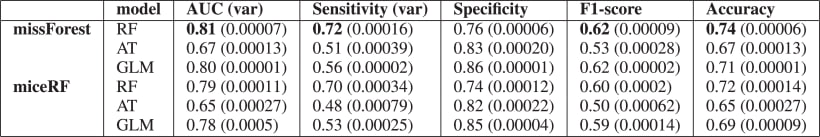
\includegraphics[width=1\linewidth]{immagini/resultCovidModels.jpg}
		\caption{Tabella con le misure di \textit{performance} calcolate usando \textit{random forest} (RF), alberi associativi derivati (AT), modelli generalizzati (GLM) (fonte \cite{Casiraghi2020-zt}).}
		\label{fig:resultcovidmodel}
	\end{figure}
	
	
	\chapter{Dataset}
	\label{Dataset}
	Un insieme di dati, \textit{dataset} in inglese, è una raccolta di dati in cui ogni riga rappresenta un'osservazione, o istanza, e ogni colonna costituisce un attributo, o caratteristica, dell'istanza. I metodi di apprendimento hanno bisogno di dati per poter addestrare modelli. L'obiettivo è riuscire a creare modelli che siano in grado di generalizzare ed effettuare previsioni affidabili sui nuovi dati. I dati possono influire significativamente sulle prestazioni delle predizioni, pertanto è importante utilizzare un insieme di dati ben equilibrato, rappresentativo e qualitativo.
	
	In questo lavoro è stato usato apprendimento supervisionato quindi l'insieme di dati aveva anche un'etichetta. L'obiettivo è stato addestrare modelli in modo che riuscissero a estrapolare la relazione che sussiste tra i dati, $X$, e l'etichetta, $y$, per far sì che, fornendo in \textit{input} nuove istanze, restituissero l'etichetta predetta sulla base dei dati passati precedentemente. 
	In questo capitolo sono stati spiegati i dati multi-omici, ovvero la tipologia di dati usata durante gli esperimenti, la fonte utilizzata per reperire i dati e approfonditi i dati impiegati. Successivamente sono state illustrate le varie fasi del preprocessing ed è stata fatta una rassegna di tutte le tecniche di di \textit{dimensionality reduction} usate durante gli esperimenti.
	
	\section{Dati Multi-Omici}
	I dati multi-omici sono un insieme che contiene le variazioni molecolari su più livelli quali: genomica, epigenomica, trascrittomica, proteomica, metabolomica e microbiotica \cite{Hasin2017}. La disponibilità di questo tipo di dati ha completamente rivoluzionato il campo della medicina e della biologia. 
	In Figura \ref{fig:multi-omics} è possibile vedere i livelli spiegati precedentemente, di seguito sono analizzati nel dettaglio.
	\begin{itemize}
		\item La genomica è il campo che si occupa dell'identificazione dei geni e delle varianti geniche associate a una malattia o in risposta a determinati medicinali.
		
		\item L'epigenomica è il campo dell'identificazione di modificatori di DNA o delle proteine associate al DNA. Le modifiche epigenetiche del genoma possono anche agire come marcatori per sindromi metaboliche, malattie cardiovascolari e disturbi fisiologici. Queste modifiche possono essere specifiche per cellula e tessuto: è quindi fondamentale identificare le modifiche epigenetiche durante gli stati nativi della malattia.
		
		\item La trascrittomica è il campo che studia le proprietà associate alla produzione di RNA dal DNA. L'obiettivo di questa area di ricerca è la comprensione di come il DNA venga trascritto in RNA. Sebbene solo il $2\%$ del DNA venga tradotto in proteine, quasi l'$80\%$ del genoma viene trascritto e tale processo include RNA codificante, RNA corto \cite{lee2004short}, microRNA \cite{lu2018microrna}, \textit{piwi} RNA \cite{ozata2019piwi} e piccoli RNA nucleari \cite{cullen2003nuclear}. Lo studio della trascrittomica può aiutare a identificare molti problemi di salute, tra cui: cancro \cite{sager2015transcriptomics}, malattie neurodegenerative (come l'Alzheimer \cite{papassotiropoulos2006genetics}), infiammatorie \cite{chan2018delineating} e metaboliche \cite{stenton2020diagnosis}.
		
		\item  La proteomica è il campo nel quale si cerca di identificare gli strati, le modifiche e le interazioni delle proteine a livello del genoma. Queste modifiche sono coinvolte nella manutenzione della struttura e della funzione cellulare. 
		
		\item Il metaboloma è l'insieme di tutti i metaboliti presenti in una cellula, tessuto o organismo, compresi piccoli molecolari, carboidrati, peptidi, lipidi, nucleotidi e i prodotti catabolici. Rappresenta il prodotto finale della trascrizione genica e consiste sia in molecole di segnalazione sia strutturali. La dimensione del metaboloma è molto più piccola rispetto alla dimensione del proteoma e quindi è più facile da studiare.
		
		\item La microbiomica consiste in tutti i microorganismi di una comunità. I microbi sono ovunque: sono stati trovati sulla pelle umana, sulle superfici mucose e nell'intestino. Il microbioma presente negli esseri umani, oltre che molto diffuso, è molto complesso, ad esempio nell'intestino troviamo circa 100 trilioni di batteri \cite{microbiota}.
		La microbiota è stata trovata coinvolta in diabete, obesità, cancro, colite, malattie cardiache e autismo. Pertanto la caratterizzazione del microbioma di un organismo è di grande interesse medico.
	\end{itemize}
	
	Grazie alla ricerca ci sono stati importanti progressi in diversi campi omici e si è capito che la risposta a una domanda in medicina non è da ricercare in un solo tipo di dato poiché questi dati si influenzano tra di loro: per esempio il microbioma influenza l'espressione genica e proteica che a sua volta influenza il metabloma. È quindi necessario studiare i dati nella loro interezza sfruttando i dati multi-omici per comprendere lo stato nativo e alterato di un organismo attraverso l'analisi dei dati provenienti da diverse fonti omiche.
	
	\begin{figure}[t]
		\centering
		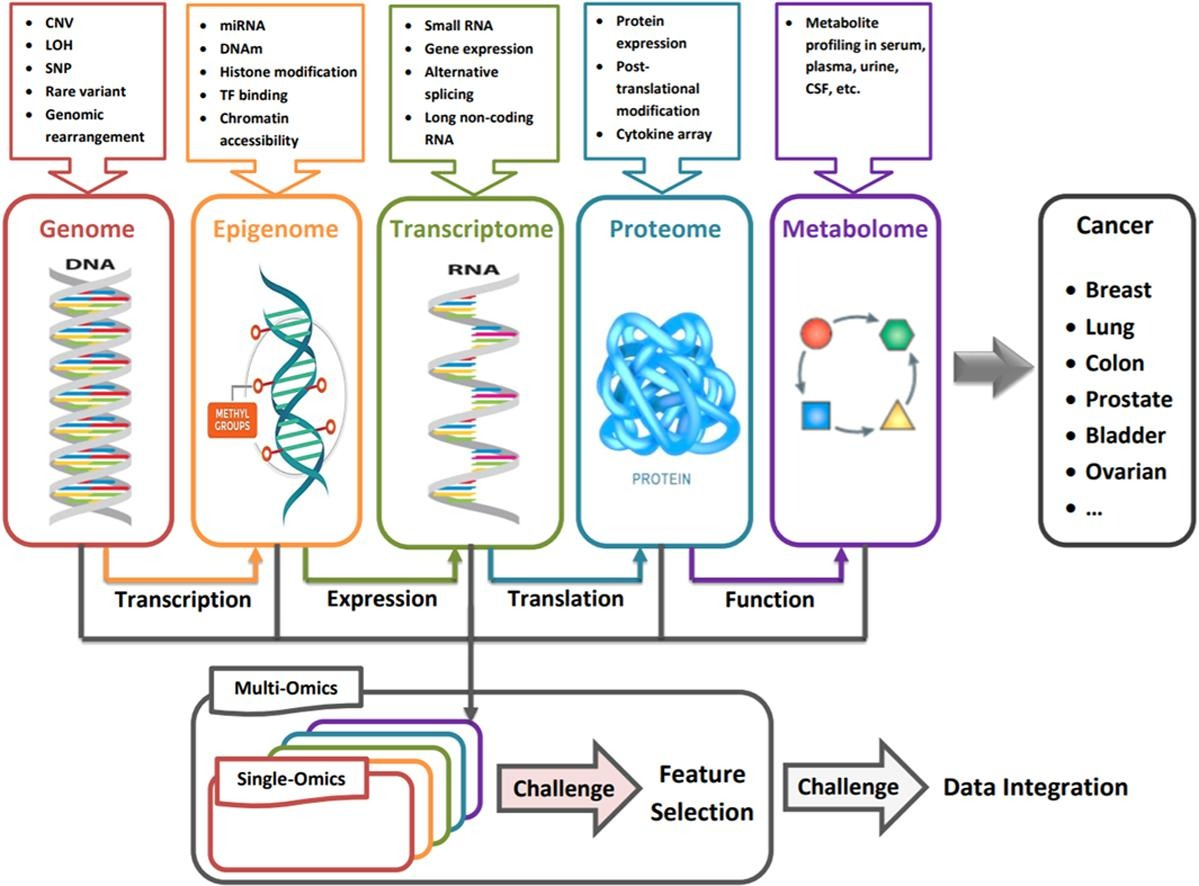
\includegraphics[width=0.9\linewidth]{immagini/multi-omicsData}
		\caption{Diagramma delle relazioni tra i vari tipi di dati omici (fonte: \cite{MOMENI2020103466}).}
		\label{fig:multi-omics}
	\end{figure}
	
	Esistono diversi database che forniscono dati multi-omici di pazienti, uno di questi è il \textit{The Cancer Genome Atlas}.
	
	\subsection{The Cancer Genome Atlas (TCGA)}
	Il \textit{Cancer Genome Atlas} \cite{TCGASource} è il programma scientifico  di riferimento per la genomica del cancro e ha favorito la caratterizzazione sistematica di diverse alterazioni genomiche alla base dei tumori umani. Attualmente ha caratterizzato oltre 11000 tumori di 33 tipi di cancro. Si tratta di uno sforzo congiunto tra \textit{Nation Cancer Institute} e il \textit{National Human Genome Research Institute} e riunisce ricercatori di diverse discipline e istituzioni di ogni parte del mondo.


	I dati forniti sono composti da 627 pazienti e di ognuno sono presenti i dati relativi a proteine, CNV, mRNA, miRNA e la relativa etichetta (che indica la presenza o assenza di evento tumorale). I primi 3 tipi di dati sono stati presi da TCGA tramite il \textit{package} \textit{curatedTCGAData}\footnote{https://bioconductor.org/packages/release/data/experiment/html/curatedTCGAData.html} da Bioconductor\footnote{La missione del progetto Bioconductor è quella di sviluppare, supportare e diffondere software open source gratuito che faciliti un'analisi rigorosa e riproducibile dei dati provenienti da saggi biologici attuali ed emergenti.}. Essi sono dati sul carcinoma mammario invasivo (TCGA-BRCA). Questo è un tipo di cancro che si sviluppa all'interno della mammella ed è in grado di diffondersi alle altri parti del corpo attraverso linfonodi o vasi sanguigni. I dati sono stati ottenuti facendo riferimento alla versione del genoma umano hg19: questa versione è stata pubblicata nel 2009 dal progetto internazionale del genoma umano (IGHP)\footnote{https://www.genome.gov/human-genome-project} e contiene informazioni su sequenza del DNA umano, sequenze dei geni, i siti di regolazione genica e le regioni non codificanti del DNA. 
	Per quanto riguarda invece le etichette sono state prese da un \textit{dataset} noto come TCGA-CDR \cite{LIU2018400}, curato manualmente per avere dati clinici e di sopravvivenza il più affidabili possibile.
	Nei paragrafi che seguono sono stati approfonditi tali dati.
	
	\paragraph{Proteine}
	\label{Proteine}
	Le proteine sono le macromolecole che svolgono essenzialmente ogni compito all'interno della cellula. Questi dati rappresentano i loro livelli di espressione.  Tra i loro compiti, quelli più importanti sono:
	\begin{itemize}
		\item strutturali: alcune proteine formano la struttura delle membrane cellulari e altre sostengono la forma della cellula,
		\item catalitici: molte proteine sono enzimi che catalizzano reazioni chimiche all'interno della cellula,
		\item regolatori: alcune proteine regolano l'espressione genica e la risposta allo stress,
		\item di trasporto: alcune proteine fungono da trasportatori di ioni e molecole attraverso la membrana cellulare,
		\item immunitari: alcune proteine fungono da anticorpi che proteggono la cellula da agenti esterni,
		\item comunicativi: alcune proteine fungono da messaggeri chimici che comunicano tra le cellule.
	\end{itemize}
	I dati utilizzati durante gli esperimenti sono stati ottenuti con una tecnica nota come RPPA \cite{Coarfa2021-eh} (\textit{Reverse Phase Protein Array}).
	
	\paragraph{mRNA}
	\label{mRNA}
	RNA messaggero (noto con l'abbreviazione di mRNA o con il termine più generico di trascritto) è una delle principali molecole in grado di trasportare l'informazione genetica dal nucleo della cellula, dove si trova il DNA, al citoplasma, dove avviene la sintesi proteica. I dati indicano i suoi livelli di espressione. Essi sono ottenuti tramite una tecnica chiamata \textit{RNA-sequencing} \cite{Wang2009-wi}. 
	
	\paragraph{miRNA}
	\label{miRNA}
	microRNA, noto con l'abbreviazione di miRNA, sono piccoli RNA (non codificanti per proteine) che svolgono funzioni di regolazione all'interno della cellula.
	I dati indicano i suoi livelli di espressione. Essi sono ottenuti, come per mRNA, tramite \textit{RNA-sequencing}.
	
	\paragraph{CNV}
	\label{CNV}
	\textit{Copy Number Variants} (CNV), o varianti nel numero di copie, sono le varianti genetiche, tra cui inserzioni, delezioni e duplicazioni di segmenti di DNA. I dati si riferiscono al tratto genetico che coinvolge il numero di copie di un particolare gene presente nel genoma di un individuo.  Per ogni gene viene indicato se lo stesso abbia subito delezione (come la perdita di una o più copie), amplificazione (acquisizione di una	o più copie), neutro (nessuna modifica). I dati possono può assumere i seguenti valori: 0 (neutro), 1 o 2 (amplificazioni), -1 o -2 (delezioni).
	
	\paragraph{Etichetta}
	\label{Etichetta}
	Rappresentano la $y$ descritta nel Paragrafo \ref{SupervisedLearning}. In Figura \ref{fig:distribuzionedati} è possibile vedere un diagramma a barre che mostra come i dati sono distribuiti tra sani e malati. Le etichette fanno riferimento a una misura nota come PFI (\textit{Progression Free Interval}) dove: 
	\begin{itemize}
		\item 1 indica che il paziente ha un nuovo evento tumorale, che sia una progressione della malattia, una recidiva locale, una metastasi a distanza, nuovi tumori primari in tutti i siti o sia morto con il cancro senza nuovo evento tumorale, compresi i casi con un nuovo evento tumorale il cui tipo è N/A,
		\item 0 indica che il paziente non ha avuto alcun evento tumorale.
	\end{itemize}

	\begin{figure}[h]
		\centering
		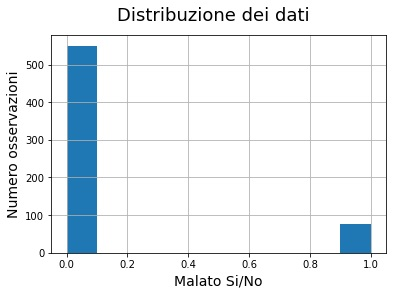
\includegraphics[width=0.7\linewidth]{immagini/distribuzioneDati}
		\caption{Istogramma che mostra quanti pazienti risultano malati in base a una misura nota come PFI (\textit{Progression Free Interval}) in cui: 1 sta a indicare la presenza di un evento tumorale in un paziente (colonna di destra); 0 l'assenza di un evento di questo tipo (colonna di sinistra).}
		\label{fig:distribuzionedati}
	\end{figure}
	
	
	\section{Preprocessing}
	\label{preprocessing}
	La prima fase del lavoro ha riguardato la manipolazione dei dati per renderli di più facile analisi e interpretazione per l'utilizzo dell'algoritmo che verrà applicato successivamente. Questo processo è importante poiché i dati grezzi spesso non sono adatti per l'algoritmo scelto e questo può influire sulle prestazioni finali.
	Di seguito sono illustrati i diversi passaggi del \textit{preprocessing}.
	\begin{itemize}
		\item Codifica: processo di gestione delle variabili categoriche. Ciò consiste nel trasformare queste variabili non numeriche in una rappresentazione numerica utilizzabile dai modelli di \textit{machine learning}. 
		
		\item Normalizzazione dei dati: consiste nel trasformare i valori di una o più variabili usando una scala comune. Questo viene fatto poiché all’interno del \textit{dataset} potrebbero esserci variabili che usano scale diverse. Prendiamo per esempio un dataset con all’interno due variabili numeriche, ``altezza'' e ``peso'': ovviamente non usano la stessa scala, la prima si misura in centimetri e la seconda in kg.
		
		\item Pulizia dei dati: consiste nella rimozione di valori duplicati, valori completamente fuori scala, detti \textit{outlier} e valori mancanti o nulli. Questi ultimi possono anche essere imputati. L'imputazione è il processo di sostituzione di questo tipo di dati con valori sintetici. Questa pratica viene utilizzata poiché molti algoritmi di \textit{machine learning} non possono gestire valori mancanti e il loro effetto sulle prestazioni dei modelli può essere significativo. Esistono diverse tecniche per fare imputazione di dati. Alcuni esempi sono: \textit{mean imputation}, \textit{median imputation}, \textit{regression imputation}, \textit{k-nearest neighbors (KNN)}, \textit{multiple imputation} (\cite{doi:10.1080/08839514.2019.1637138, waljee2013comparison}).
		
		\item \textit{Dimensionality reduction}: consiste nella riduzione del numero di caratteristiche di un \textit{dataset} ad alta dimensionalità in uno a più bassa dimensionalità pur mantenendo il più possibile l'informatività dei dati. Questo processo consente di ridurre la complessità del modello, migliorare la sua capacità di generalizzazione e la precisione delle previsioni.
		La riduzione della dimensionalità può essere fatta in diversi modi, usando tecniche di \textit{feature selection}, \textit{feature extraction} o tecniche come t-SNE, algoritmo di visualizzazione non lineare utilizzato per ridurre la dimensione di un \textit{dataset} in uno spazio a bassa dimensione, pur mantenendo le relazioni di prossimità tra i punti. Il primo modo consiste nella selezione delle caratteristiche; ovvero nella scelta delle variabili, o \textit{feature} appunto, più rilevanti per il modello di \textit{machine learning}, al fine di ridurre la complessità del modello, migliorare la sua capacità di generalizzazione e accelerarne la convergenza durante l'addestramento. Il secondo modo consiste nel costruire nuove \textit{feature} in funzione di quelle di partenza.
	\end{itemize}
	
	
	\section{Riduzione della dimensionalità}
	Negli ultimi anni i dati disponibili per applicazioni di \textit{machine learning} in ambiti come \textit{mining} di testo, \textit{computer vision} e biomedico stanno aumentando esponenzialmente sia in termini di campioni sia in termini di numero di dimensioni. L'enorme numero di \textit{feature} dei \textit{dataset} attualmente disponibili porta diversi svantaggi: rallentamento significativo degli algoritmi di \textit{learning}, peggioramento della \textit{performance} dei suddetti algoritmi e difficoltà nell'interpretazione del modello. Molto spesso i \textit{dataset} che vengono utilizzati per il \textit{machine learning} hanno un'elevata dimensionalità, basti pensare che i \textit{dataset} usati negli esperimenti hanno $627$ osservazioni (ovvero i pazienti) e un numero di \textit{feature} molto elevato (vedi Tabella \ref{numero_feature}).
	\begin{table}[]
		\begin{center}
			\begin{tabular}{l|llll}
				\hline
				&  Proteine&mRNA  &miRNA  &CNV  \\ \hline
				numero di \textit{feature}&  216&20501  &1046  &24776 
			\end{tabular}
		\end{center}
		\caption{Tabella che illustra il numero di  \textit{feature} per ogni \textit{dataset} fornito.}
		\label{numero_feature}
	\end{table}
	Per gestire adeguatamente questi dati del mondo reale è necessario ridurne la dimensionalità. La riduzione della dimensionalità è la trasformazione di dati ad alta dimensione in una rappresentazione significativa di dimensionalità ridotta \cite{van2009dimensionality}. Idealmente, la rappresentazione ridotta dovrebbe avere una dimensionalità che corrisponde alla dimensionalità intrinseca dei dati (vedi Paragrafo  \ref{IntrinsicDimension}). Esistono diversi modi per eseguire riduzione della dimensionalità: in questo lavoro sono state usate tecniche di \textit{feature selection}, \textit{feature extraction}.
	La riduzione della dimensionalità è importante in molti domini, poiché attenua la \textit{curse of dimensionality} \cite{Keogh2017} e altre proprietà desiderate degli spazi ad alta dimensionalità \cite{Jimenez1998SupervisedCI}. La riduzione della dimensionalità facilita la classificazione, la visualizzazione e la compressione di dati ad alta dimensionalità. Esistono diverse tecniche lineari come \textit{Principal Component Analysis} (PCA) \cite{ringner2008principal}, \textit{Linear Discriminant Analysis} (LDA) \cite{balakrishnama1998linear} e \textit{Singular Value Decomposition} (SVD) \cite{wall2003singular}. Tuttavia queste tecniche lineari non sono in grado di gestire adeguatamente dati complessi e non lineari.
	Esistono tecniche di riduzione della dimensionalità non lineari che vengono utilizzate in molti casi in cui i dati hanno una struttura non lineare e non possono essere adeguatamente rappresentati mediante tecniche lineari di riduzione della dimensionalità, i più noti sono UMAP (\textit{Uniform Manifold Approximation and Projection}) (\textit{feature extraction}) e t-SNE (\textit{t-distributed Stochastic Neighbor Embedding}).
	\subsection{t-SNE: t-distributed Stochastic Neighbor Embedding}
	\label{t-sne}
	t-SNE è una tecnica di riduzione della dimensionalità non lineare introdotta in Van der Maaten et al.\cite{van2008visualizing}. Essendo una tecnica non lineare è in grado di separare dati che non possono essere separati da una linea retta. La Figura \ref{fig:t-sneImageAll} ne riporta un esempio.
	
	\begin{figure}
		\centering
		\begin{subfigure}[b]{0.49\textwidth}
			\centering
			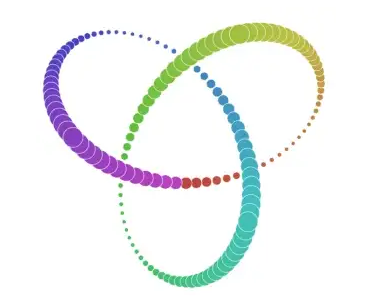
\includegraphics[width=0.9\linewidth]{immagini/t-SNEImage}
			\caption{}
			\label{fig:t-sneimage}
		\end{subfigure}
		\begin{subfigure}[b]{0.49\textwidth}
			\centering
			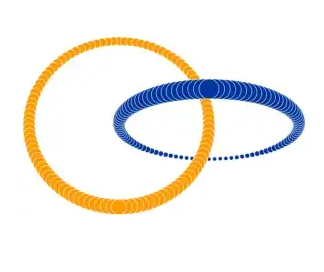
\includegraphics[width=1\linewidth]{immagini/t-SNEImage2}
			\caption{}
			\label{fig:t-sneimage2}
		\end{subfigure}
		\caption{Esempi di dati non separabili linearmente (fonte: \cite{tnseDatiNonSeparabili} CC-BY 2.0).}
		\label{fig:t-sneImageAll}
	\end{figure}
	Di seguito sono elencate le diverse fasi dell'algoritmo.
	\begin{itemize}
		\item Inizialmente viene creata una distribuzione di probabilità che rappresenta la similarità tra i vicini. La similarità tra due punti $x_i$ e $x_j$ è la probabilità condizionale $P_{j|i}$ che $x_i$ sceglierebbe $x_j$ come suo vicino se i vicini venissero scelti in base alla funzione di densità di probabilità sotto una gaussiana centrata in $x_i$ \cite{van2008visualizing}. Successivamente viene calcolata la distanza euclidea per ogni punto appartenente al \textit{dataset}. Dopo un processo di normalizzazione, quello che si ottiene è un insieme di valori di probabilità $P_{i,j}$ che sono proporzionali ai valori di similarità. La distribuzione può essere manipolata usando quella che viene chiamata ``perplessità'', la quale è, più o meno, un numero target di vicini per il nostro punto centrale. In pratica, più alta è la perplessità, più alto è il valore della varianza, ovvero quanto è ampia la curva. 
		
		\item Successivamente viene ripetuto il processo descritto precedentemente ma questa volta al posto di una distribuzione gaussiana viene usata una t-Student. Questa nuova distribuzione ci fornisce un nuovo insieme di probabilità $Q_{ij}$ ma in uno spazio ridotto. Come visibile in Figura \ref{fig:t-distribution}, la distribuzione t-Student ha code più lunghe rispetto a una distribuzione gaussiana e ciò consente di visualizzare più facilmente le distanze tra i punti.
		
		\item Infine si procede a calcolare le probabilità $Q_{ij}$ nello spazio ridotto in modo tale che esse riflettano nella maniera più precisa possibile le probabilità $P_{ij}$ relative allo spazio iniziale a dimensioni più elevate.  Questo procedimento viene svolto misurando la differenza tra le due distribuzioni di probabilità usando la divergenza di Kullback-Liebler \cite{joyce2011kullback} che è in grado di confrontare i valori di $P_{ij}$ e $Q_{ij}$. Per minimizzare la divergenza tra le due dimensioni viene utilizzata la \textit{gradient descent} \cite{https://doi.org/10.48550/arxiv.1609.04747, van2008visualizing}.
	\end{itemize}
	
	
	\begin{figure}
		\centering
		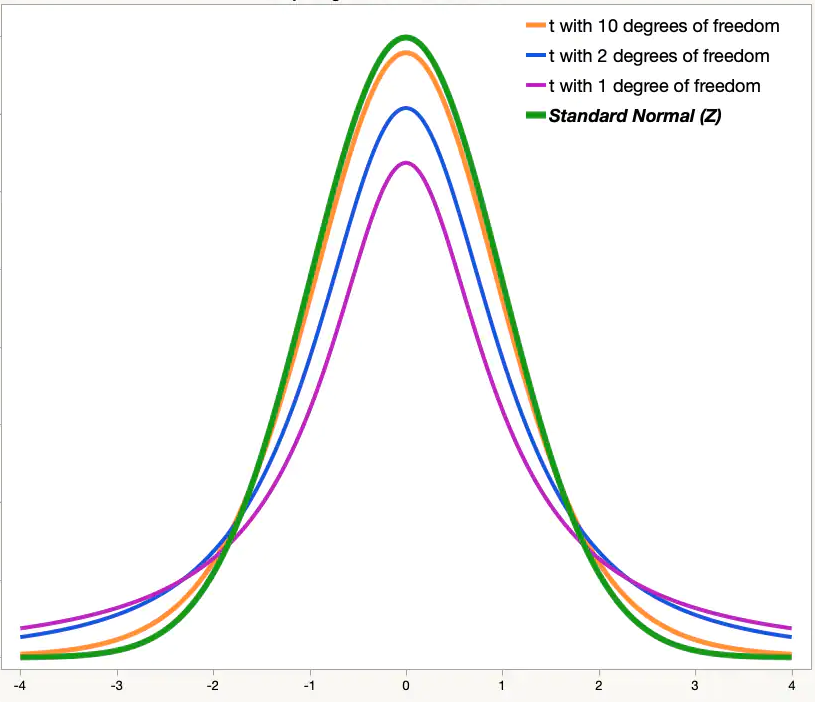
\includegraphics[width=0.65\linewidth]{immagini/t-distribution}
		\caption{Grafici della densità delle distribuzioni gaussiane (in verde) e t-Student (in arancione, blu e viola) a seconda dei gradi di libertà ovvero al numero di osservazioni indipendenti all'interno del \textit{dataset} di partenza (fonte \cite{t-studentFunction}).}
		\label{fig:t-distribution}
	\end{figure}
	
	\subsection{Feature Extraction}
	La \textit{feature extraction} è una tecnica di riduzione della dimensionalità che consiste nella creazione di nuove \textit{feature} in funzione delle variabili di partenza. L'obiettivo è sempre quello di migliorare le prestazioni di apprendimento automatico o, in generale, semplificare il modello. Tra le tecniche di \textit{feature extraction} le più note sono: \textit{Principal Component Analysis}(PCA) \cite{abdi2010principal}, \textit{Linear Discriminant Analysis} (LDA) \cite{balakrishnama1998linear},  \textit{Singular Value Decomposition} (SVD)\cite{abdi2007singular} e UMAP, illustrato nel Paragrafo seguente.
	
	
	\subsubsection{UMAP: Uniform Manifold Approximation}
	\label{Umap}
	UMAP \cite{https://doi.org/10.48550/arxiv.1802.03426} è un algoritmo di riduzione della dimensionalità non lineare il cui scopo è rappresentare dati ad alta dimensionalità in uno spazio a bassa dimensione cercando di preservare le relazioni topologiche e spaziali tra i punti dei dati. Centrale è il concetto di \textit{manifold}: chiamata varietà in italiano, si tratta di uno spazio topologico che localmente è simile a uno spazio topologico ben conosciuto (ad esempio lo spazio euclideo $n$-dimensionale), ma che globalmente può avere proprietà geometriche differenti (ad esempio può essere curvo contrariamente allo spazio euclideo). Per esempio, una superficie sferica è un \textit{manifold} di dimensione 2 in uno spazio tridimensionale. Una curva può essere vista come un \textit{manifold} di dimensione 1 in uno spazio a due dimensioni. La Figura \ref{fig:manifoldexample} riporta un esempio di questo fatto, considerando la superficie terrestre.
	\begin{figure}[h]
		\centering
		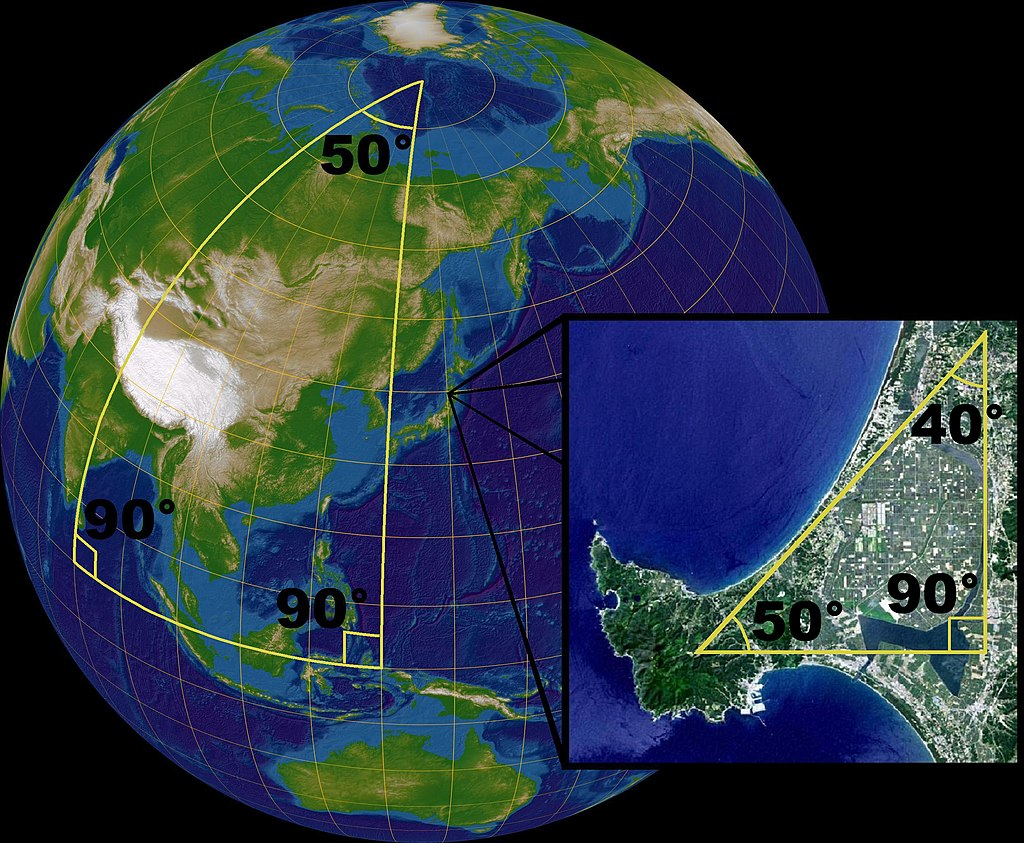
\includegraphics[width=0.6\linewidth]{immagini/ManifoldExample}
		\caption{Localmente la superficie terrestre somiglia a un piano, e per questo è una varietà di dimensione 2. Tuttavia tale somiglianza non conserva la distanza tra i punti, in quanto la sfera ha una curvatura diversa. La curvatura incide sulla somma degli angoli interni di un triangolo: nel piano tale somma è sempre 180°, mentre su una sfera è sempre maggiore. Ad esempio, la somma degli angoli interni del triangolo in figura è 230°. La figura in basso a destra è un triangolo in senso euclideo ma non rispetto alla geometria della sfera, in quanto i suoi lati non rappresentano delle geodetiche della sfera (fonte: \cite{manifold} Dual-licensed under the GFDL and CC-By-SA).}
		\label{fig:manifoldexample}
	\end{figure}
	In termini di analisi dei dati, UMAP considera che molti \textit{dataset} ad alta dimensionalità siano distribuiti su un \textit{manifold} sottostante di dimensione inferiore. L'idea è che le proprietà dei dati siano meglio descrivibili da questo \textit{manifold} sottostante piuttosto che dallo spazio completo ad alta dimensionalità.
	
	L'algoritmo UMAP funziona attraverso due fasi principali:
	\begin{itemize}
		\item approssimazione uniforme delle strutture di \textit{manifold}: UMAP utilizza una combinazione di tecniche di apprendimento non supervisionato, come la costruzione di un grafo di vicinato e l'utilizzo di una funzione di costo, per approssimare la struttura dei dati ad alta dimensionalità;
		\item proiezione su uno spazio a bassa dimensione: dopo aver approssimato la struttura dei dati, UMAP utilizza una tecnica di proiezione non lineare per rappresentare i dati in uno spazio a bassa dimensione, mantenendo le relazioni topologiche e spaziali.
	\end{itemize}
	UMAP utilizza un metodo di costruzione e incorporazione di grafi non lineari per ottimizzare un obiettivo che consente un compromesso tra l'enfatizzazione delle strutture locali e la conservazione delle distanze a livello globale. Questo compromesso è controllato principalmente dai parametri \textit{n\_neighbors} e \textit{min\_dist} di UMAP. 
	Il parametro \textit{n\_neighbors} controlla il numero di vicini di cui viene preservata la topologia locale, le distanze globali vengono preservate quando è alto. Il parametro \textit{min\_dist} controlla la distanza minima tra i campioni nell'incorporazione e ciò influisce sulla diffusione dei \textit{cluster}. Valori bassi di \textit{min\_dist} consentono a UMAP di enfatizzare la somiglianza di gruppi densi di campioni, mentre valori più grandi si concentrano sulla conservazione di distanze più ampie.
	
	\subsection{Feature selection}
	\label{FeatureSelection}
	Nel \textit{machine learning}, e in statistica, con il termine \textit{feature selection} si intende il processo di selezione di un sottoinsieme di \textit{feature}, chiamate anche caratteristiche, dimensioni o variabili, rimuovendo quelle irrilevanti, ridondanti o che producono solo rumore \cite{featureSelection}. Questa pratica, di solito, porta a una migliore capacità di addestramento, accuratezza più elevata, minore costo computazionale e aumento dell'interpretabilità del modello. La \textit{feature selection} aiuta anche a non incappare nel \textit{curse of dimensionality}.
	

	Esistono diverse tecniche per effettuare \textit{feature selection} le quali possono essere di tipo univariato o multivariato. La differenza tra queste tecniche risiede in come vengono valutate le \textit{feature}. Le tecniche univariate valutano l'importanza di ogni \textit{feature} in modo indipendente dalle altre. Queste tecniche sono indubbiamente più facili da implementare e comprendere rispetto a quelle multivariate ma potrebbero ignorare completamente le relazioni tra le variabili e selezionare \textit{feature} inutili. Le tecniche multivariate valutano l'importanza di una \textit{feature} confrontandola con tutte le altre \textit{feature}. Al contrario delle tecniche univariate, le tecniche multivariate sono più adatte per dataset con molte \textit{feature} ma possono essere più complesse da implementare e comprendere rispetto alle tecniche univariate \cite{goswami2014feature}. Infine le tecniche multivariate risultano molto più costose a livello computazionale.
	Di seguito vengono approfondite le tecniche usate durante gli esperimenti.
	
	\subsubsection{L'indice di correlazione di Pearson}
	\label{Pearson}
	L'indice di correlazione di Pearson è un metodo che misura la correlazione lineare tra due variabili, spesso indicato con $\rho$ \cite{Benesty2009}. Viene calcolato come il rapporto tra la covarianza di due variabili e il prodotto delle loro deviazioni standard ed è sempre compreso tra $-1$ e $1$.
	Data una coppia di variabili casuali $(X,Y)$ è possibile calcolare $\rho$ con la formula seguente:
	\begin{equation}
		r_{xy} = \frac{\text{cov}(X,Y)}{\sigma_x \cdot \sigma_y},
	\end{equation}

	
	dove:
	\begin{itemize}
		\item $r_{xy}$ è l'indice di correlazione di Pearson tra le variabili $X$ e $Y$,
		\item $\text{cov}(X,Y)$ è la covarianza tra le variabili $X$ e $Y$,
		\item $\sigma_x$ e $\sigma_y$ sono la deviazione standard delle variabili $X$ e $Y$.
	\end{itemize}
	
	Parlando dell'indice di correlazione di Pearson è bene definire due concetti: \textit{cut-off} e \textit{p-value}. Il primo viene utilizzato per stabilire se esiste o meno una correlazione significativa tra due variabili. Il \textit{cut-off} viene solitamente stabilito in base al livello di significatività desiderato e può variare tra i diversi studi. Un valore di \textit{cut-off} comune è $0.8$, il che significa che una correlazione con un valore di indice di Pearson superiore a $0.8$ è considerata significativa e indica una correlazione lineare forte tra due variabili. In questo caso potrebbe essere opportuno scartare una delle due variabili, poiché potrebbe essere considerata ridondante. Tuttavia, la scelta dipende dal contesto specifico del problema e dalla comprensione che si ha delle relazioni tra le variabili.
	
	Il secondo, invece, indica la probabilità che la correlazione osservata tra le due variabili sia dovuta al caso. Un \textit{p-value} basso, solitamente inferiore a $0.05$, indica che la correlazione è significativa e che non è probabile che sia stata generata casualmente. Al contrario, un \textit{p-value} elevato indica che la correlazione potrebbe essere dovuta al caso e che non c'è sufficiente evidenza per supportare l'esistenza di una correlazione significativa.
	
	In altre parole, il \textit{p-value} fornisce una misura del livello di significatività statistica della correlazione tra le variabili. Se il \textit{p-value} è inferiore a un certo livello di significatività, si può rifiutare l'ipotesi nulla e concludere che esiste una correlazione significativa tra le variabili.
	L'ipotesi nulla, spesso indicata con $H_0$, è un'affermazione che viene sfidata per essere confermata o smentita tramite i dati a disposizione. L'ipotesi nulla viene accettata finché non è evidente che valga l'ipotesi opposta, ovvero quella alternativa, indicata con $H_1$. Ovvero:
	\begin{itemize}
		\item ipotesi nulla $H_0: P(X \geq Y) = P(Y \geq X)$,
		\item ipotesi alternativa $H_1: P(X \geq Y) \neq P(Y \geq X)$.
	\end{itemize}
	
	L'ipotesi nulla viene rifiutata quando il \textit{p-value} è minore di un determinato livello di significatività prefissato (tipicamente $0.05$). Il rifiuto dell'ipotesi comporta che ci sia evidenza tale che i dati non riescono a fornire abbastanza prove a favore dell'ipotesi nulla.
	
	
	È bene notare che il \textit{p-value} e il \textit{cut-off} sono entrambi utilizzati per stabilire se una correlazione sia significativa o meno, ma il \textit{p-value} fornisce una misura quantitativa della probabilità che i risultati ottenuti siano casuali, mentre il \textit{cut-off} è un valore soglia fissato arbitrariamente.
	
	\subsubsection{Il coefficiente di Spearman}
	Il coefficiente di correlazione di rango Spearman è una misura non parametrica della monotonicità della correlazione tra due variabili ordinali o tra due variabili quantitative con una distribuzione non-normale. Il coefficiente di correlazione di Spearman è simile al coefficiente di correlazione di Pearson, ma è più adatto per i dati non-normali o ordinali, poiché non richiede che le variabili siano normalmente distribuite. I valori variano tra $-1$ e $+1$ con $0$ che implica una correlazione debole o assente. Le correlazioni con valori $-1$ implicano una correlazione negativa forte mentre quelle con valori $+1$ implicano una correlazione positiva forte \cite{spearman}. Anche in questo caso, come con l'indice di Pearson, potrebbe essere opportuno scartare una delle due variabili altamente correlate, poiché potrebbe essere ridondante.
	
	Nella correlazione di Spearman il \textit{p-value} viene utilizzato per determinare se la correlazione tra le due variabili sia significativa o meno. Se il \textit{p-value} è inferiore a un livello di significatività prestabilito (nel mio lavoro ho usato $0.05$) si può dire che la correlazione è significativa.  Al contrario, se il \textit{p-value} è maggiore di un certo livello di significatività, non c'è evidenza sufficiente per affermare che la correlazione sia significativa. In sintesi, l'indice di correlazione di Spearman fornisce informazioni quantitative sulla forza della correlazione tra le variabili, mentre il \textit{p-value} fornisce informazioni sul significato statistico della correlazione.
	Il coefficiente viene così calcolato:
	\begin{equation}
		\rho = 1 - \frac{6 \sum d_i^2}{n(n^2 - 1)},
	\end{equation}
	dove:
	\begin{itemize}
		\item $\rho$ è il coefficiente di correlazione di Spearman,
		\item $n$ è il numero di osservazioni,
		\item $d_i$ è la differenza tra la posizione della i-esima osservazione nella prima variabile e nella seconda variabile, ordinate in modo crescente.
	\end{itemize}

	
	\subsubsection{Il test di Mann-Whitney}
	\label{Mannwhitney}
	Il test $U$ di Mann-Whitney, anche noto con il nome di test della somma dei ranghi di Wilcoxon o test U di Mann-Whitney, è un test non parametrico dell'ipotesi nulla. Questo test viene spesso utilizzato per determinare se esiste una differenza significativa tra le medie di due gruppi, indipendentemente dalla loro distribuzione di probabilità.
	Una formulazione generale del test $U$ consiste nell'assumere che:
	\begin{itemize}
		\item tutte le osservazioni provenienti da due gruppi siano indipendenti l'uno dall'altro,
		\item prese due osservazioni, si possa dire quale sia la maggiore. I valori dovrebbero essere ordinali,
		\item sotto l'ipotesi nulla $H_0$, le distribuzioni delle due popolazioni siano identiche,
		\item l'ipotesi alternativa $H_1$ dice che le distribuzioni non siano identiche.
	\end{itemize}
	Secondo le assunzioni fatte precedentemente, il test è coerente quando: per valori estratti uniformemente a caso $X$ e $Y$, si verifica se la probabilità che $X$ sia maggiore di $Y$ sia uguale alla probabilità che $Y$ sia maggiore di $X$.  
	
	Il test viene usato per selezionare quindi le \textit{feature} che hanno un valore di \textit{p-value}, rispetto all'etichetta per cui si vuole classificare, minore di una certa soglia (nel mio caso $0.05$). Tutte le \textit{feature}, invece, che hanno un valore di \textit{p-value} superiore vengono scartate.
	
	\subsubsection{Minimum Redundancy Maximum Relevance: mRMR}
	\label{mrmr}
	Proposto da Peng at al. \cite{1453511} la \textit{Maximum Relevance and Minimum Redundancy} (mRMR) è una tecnica di \textit{feature selection } multivariata che utilizza l'informazione reciproca\footnote{L'informazione reciproca (MI, dall'inglese \textit{Mutual Information}) è una misura di correlazione non lineare tra due variabili. Essa quantifica la quantità di informazione che una variabile fornisce sull'altra e viceversa.}, la correlazione o i punteggi di similarità/distanza per selezionare le caratteristiche di un \textit{dataset}. L'obiettivo è quello di penalizzare una \textit{feature} in base a quanto sia ridondante rispetto alle altre \textit{feature} selezionate e premiarla in base a quanto sia pertinente. Vengono quindi selezionate \textit{feature} che hanno un livello di pertinenza alto e un livello di ridondanza basso. 
	
	La massima rilevanza consiste nel ricercare le caratteristiche che soddisfano la formula definita in \ref{max-relevance} definita dal valore medio di tutti i valori di informazione reciproca tra le singole caratteristiche $x_i$ e la classe \textit{target} (anch'essa una caratteristica) $c$.
	\begin{equation}
		max D(S,c) = \frac{1}{|S|} \sum_{x_{i} \in S} I(f_{i};c),
		\label{max-relevance}
	\end{equation}
	dove:
	\begin{itemize}
		\item $D(S,c)$ è la funzione di selezione delle caratteristiche,
		\item $S$ è l'insieme di caratteristiche considerate,
		\item $|S|$ è il numero di elementi in $S$,
		\item $x_i$ è la i-esima caratteristica considerata,
		\item $I(x_i;c)$ è l'informazione reciproca tra la caratteristica $f_i$ e la classe \textit{target} $c$.
	\end{itemize}
	È probabile che le caratteristiche selezionate in base alla massima rilevanza possano avere una forte ridondanza, ovvero che la dipendenza tra queste caratteristiche possa essere molto elevata. Quando due caratteristiche dipendono molto l'una dall'altra, la corrispondente forza discriminatoria della classe non cambierebbe molto se una di queste venisse rimossa. Pertanto, in modo da selezionare le caratteristiche mutuamente esclusive, è bene aggiungere la seguente condizione di minima ridondanza (Min-Redundancy) \ref{min-redundancy}:
	\begin{equation}
		min R(S), R=\frac{1}{|S^2|}\sum_{x_i, x_j \in S}^{} I(x_i, x_j).
		\label{min-redundancy}
	\end{equation}
	Il criterio che combina i due vincoli di cui sopra viene chiamato ``minima-ridondanza-massima-rilevanza'' (mRMR). Definiamo l'operatore $\Phi(D,R)$ per combinare $D$ e $R$ e consideriamo la seguente forma più semplice per ottimizzare $D$ e $R$ contemporaneamente, quello che otteniamo è il seguente indice:
	\begin{equation}
		max \Phi(D,R), \Phi = D - R.
		\label{indice}
	\end{equation}
	Nella pratica, si possono utilizzare metodi di ricerca incrementale per trovare le caratteristiche quasi ottimali definite da $\Phi$. Supponiamo di avere già l'insieme di caratteristiche $S_{m-1}$, con $m-1$ caratteristiche. Il compito è selezionare la caratteristica $m$-esima dall'insieme delle caratteristiche \{$X-S_{m-1}$\}. Ciò avviene selezionando la caratteristica che massimizza $\Phi$. L'algoritmo incrementale ottimizza la seguente condizione:
	\begin{equation}
		\max_{x_j \in X- S_{m-1}} \left[I(x_j;c) - \frac{1}{m-1} \sum_{x_i \in S_{m1}}^{} I(x_j;x_i)\right].
	\end{equation}
	L'obiettivo è riuscire a selezionare un insieme più ristretto di caratteristiche. Si selezionano quindi le caratteristiche con i punteggi di indice più alti, mentre quelle con punteggio più basso vengono scartate. Negli esperimenti (vedi Capitolo \ref{Esperimenti}) la dimensione obbiettivo è stata impostata a $100$ quindi il processo sopra descritto viene ripetuto $100$ volte e ogni volta viene selezionata la caratteristica più rilevante, così fino a che si hanno $100$
	caratteristiche.

	\subsubsection{Boruta}
	\label{boruta}
	Boruta \cite{JSSv036i11} è un algoritmo di \textit{feature selection} che utilizza un \textit{wrapper} costruito sull'algoritmo di classificazione \textit{random forest}. Quest'ultimo è un metodo \textit{ensemble} (vedi Paragrafo \ref{RandomForest}) in cui la classificazione viene effettuata tramite una votazione di più classificatori, ovvero i \textit{decision tree}. Questi alberi sono sviluppati in modo indipendente su diversi metodi di raccolta dei campioni del \textit{training set}. Per capire l'importanza di una \textit{feature} si tiene traccia della perdita di accuratezza della classificazione causata dalla permutazione casuale dei valori delle \textit{feature}. Essa viene calcolata in maniera separata per tutti gli alberi della foresta che utilizzano una specifica \textit{feature} per la classificazione.
	Successivamente vengono calcolate media e deviazione standard della perdita di accuratezza. In alternativa può essere usato \textit{Z score} come misura di importanza, calcolato dividendo la perdita di accuratezza media per la deviazione standard. Purtroppo lo \textit{Z score} non è direttamente correlato con la significatività statistica dell'importanza della \textit{feature} restituita da \textit{random forest} \cite{10.1007/11908029_58}.
	
	In Boruta, tuttavia, viene usato lo \textit{Z score} poiché tiene conto delle fluttuazioni della perdita media di accuratezza tra gli alberi della foresta. Poiché però non è possibile usare direttamente lo \textit{Z score} per misurare l'importanza, c'è la necessità di qualcosa di esterno per decidere l'importanza di una \textit{feature}, cioè elementi che posso aiutare a distinguere l'importanza che può derivare da fluttuazioni casuali. A questo scopo vengono create delle \textit{feature} che sono casuali per costruzione in quanto i valori sono ottenuti mescolando i valori della \textit{feature} originale: chiameremo queste \textit{feature} con il nome di \textit{shadow feature}. Viene poi eseguita una classificazione utilizzando tutte le \textit{feature}, comprese quelle \textit{shawod}, e calcolata la loro importanza. 
	L'importanza delle \textit{shadow feature} viene usata come riferimento per decidere quali attributi sono importanti e quali no. Siccome la misura di importanza varia a causa dalla casualità del classificatore \textit{random forest} è necessario ripetere la procedura di creazione delle \textit{shadow feature} rimescolando i valori per ottenerne di nuove.
	Riassumendo Boruta si basa sulla stessa idea che costituisce il fondamento del classificatore \textit{random forest}, ovvero: aggiungendo casualità al sistema e raccogliendo i risultati dall'insieme di campioni randomizzati si può ridurre l'impatto fuorviante dovuto alle  fluttuazioni e dalle correlazioni casuali. In questo caso, questa ulteriore casualità ci fornirà una visione più chiara di quali \textit{feature} siano veramente importanti.
	
	Di seguito sono stati illustrati i passaggi dell'algoritmo.
	\begin{itemize}
		\item Per ogni \textit{feature} viene creata una caratteristica \textit{``shadow''}, i cui valori si ottengono mescolando i valori della \textit{feature} originale,
		\item le \textit{feature shadow} generate vengono mescolate per rimuovere le loro correlazioni con l'etichetta del problema di apprendimento supervisionato che si sta affrontando,
		\item viene eseguito l'algoritmo \textit{random forest} sul \textit{dataset} contenente i dati di partenza più le \textit{feature shadow}, i punteggi calcolati vengono salvati in $Z$,
		\item viene calcolato lo score $Z$ massimo tra gli attributi $shadow$ (MZSA),
		\item le \textit{feature} con puntegggio significativamente inferiore a MZSA vengono considerate come ``non importanti'' e rimosse permanentemente dal \textit{dataset}.
		\item le \textit{feature} con importanza significativamente superiore a MZSA vengono considerate come ``importanti'',
		\item vengono rimossi tutte le \textit{shadow feature}.
		\item il procedimento viene ripetuto fino a quando l'importanza viene assegnata a tutte le \textit{feature}.
	\end{itemize}
	La complessità temporale della procedura, in casi realistici, è circa $O(P \cdot  N )$, dove $P$ e $N$ sono rispettivamente il numero di \textit{feature} e di oggetti. Questo può risultare dispendioso per grandi insiemi di dati; tuttavia, questo sforzo è essenziale per produrre una selezione statisticamente significativa di \textit{feature} rilevanti.
	
	\subsubsection{The maximal information coefficient (MIC)}
	Il \textit{Maximal Information Coefficient} (MIC) è una misura statistica usata per identificare nuove associazioni tra coppie di variabili, o \textit{feature}. I valori del MIC sono compresi nell'intervallo $0$ e $1$. Se il valore è più vicino a $1$, le due variabili hanno una relazione più stretta; se, invece, è più vicino a $0$, le due variabili hanno più probabilità di essere indipendenti. Il MIC appartiene a una classe più ampia di statistiche basate sulla \textit{Maximal Information-based Nonparametric Exploration} (MINE) \cite{Hu2016-ji}.

	
	Intuitivamente, MIC si basa sul concetto che se esiste una relazione tra due variabili, allora è possibile tracciare una griglia sullo \textit{scatter plot}\footnote{Il grafico di dispersione, detto anche \textit{scatter plot}, è un tipo di grafico in cui due variabili di un \textit{dataset} sono riportate su uno spazio cartesiano. I dati sono visualizzati tramite una collezione di punti ciascuno con una posizione sull'asse orizzontale determinato da una variabile e sull'asse verticale determinato dall'altra.} in modo da suddividere i dati per evidenziare la relazione. 
	Pertanto, per calcolare il MIC di un insieme di dati a due variabili, si esplorano tutte le griglie calcolando per ogni coppia di interi $(x,y)$ la maggiore \textit{mutual information}\footnote{La \textit{mutual information}, o mutua informazione, di due variabili casuali è una misura di dipendenza tra due variabili casuali $X$ e $Y$ che quantifica la quantità di informazione comune che le due variabili condividono.} possibile raggiunta da qualsiasi griglia $x-by-y$ applicata ai dati \cite{articleMIC}.
	Successivamente questi valori di \textit{mutual information} vengono normalizzati per garantire un confronto equo tra griglie di dimensioni diverse. Definiamo la matrice caratteristica $M = (m_{x,y})$, dove $m_{x,y}$ è la \textit{mutual information} normalizzata più alta raggiunta da qualsiasi griglia $x-by-y$, e la statistica MIC come il valore massimo in $M$.
	Il MIC è considerato una misura più robusta rispetto ad altre misure di correlazione, poiché tiene conto sia della quantità che della qualità della \textit{mutual information} tra le variabili.
	
	\subsection{Intrinsic Dimensionality}
	\label{IntrinsicDimension}
	Il concetto di \textit{Intrinsic Dimensionanality}, o dimensionalità intrinseca in italiano, definito da Bennet \cite{Bennett1969TheID} come il numero minimo di \textit{feature} necessario per generare una descrizione dei dati mantenendo la struttura ``intrinseca'' che caratterizza l'insieme dei dati in modo da minimizzare la perdita di informazione.
	La stima della dimensione intrinseca può essere un compito difficile poiché quando il numero di \textit{feature} è elevato i dati si comportano in modo controintuitivo a causa della \textit{curse of dimensionality} (vedi Paragrafo \ref{FeatureSelection}). Un ulteriore problema risiede nel fatto che negli insiemi di dati reali non tutte le \textit{feature} hanno la stessa importanza: alcune sono molte informative, altre possono essere classificate come ``rumore'', ovvero poco informative. In generale, la dimensione intrinseca viene calcolata utilizzando una serie di algoritmi che analizzano le proprietà geometriche e statistiche dei dati, come la distanza tra i punti o la loro distribuzione. Il calcolo della dimensione intrinseca può essere utilizzato per una vasta gamma di applicazioni, tra cui la riduzione delle dimensionalità, il \textit{clustering} e la classificazione.
	
	\subsubsection{Intrinsic Dimension - Two Nearest Neighbor}
	\label{two-nn}
	L'\textit{Intrinsic Dimension--Two Nearest Neighbor} (TWO-NN) è una tecnica per calcolare la dimensione intrinseca che utilizza solo le distanze ai primi due vicini più vicini di ogni punto nel \textit{dataset} \cite{Facco2017-pd}. L'algoritmo è composto dai seguenti passi:
	\begin{itemize}
		\item per ogni coppia di punti si calcola la distanza,
		\item dato un generico punto si indica con $r_1$ e $r_2$ la più piccola e la seconda più piccola distanza precedentemente calcolata,
		\item per ogni punto $i$ si calcola $\mu_i = \frac{r_2}{r_1}$,
		\item si calcola la cumulativa empirica $F^{emp}(\mu)$ ordinando i valori di $\mu$ attraverso una permutazione $\rho$ che, dato un indice $i$, restituisce la posizione del punto $i$-esimo nella sequenza ordinata rispetto ai valori di $\mu$. Si definisce quindi $F^{emp}(\mu_{\rho(i)}) \doteq \frac{i}{N}$,
		\item si calcola la regressione lineare a partire dai punti nel piano \{$(\log(\mu_i), -\log(1-F^{emp}(\mu_i))), |i=1,...,N|$\} considerando solo rette passanti per l'origine. La pendenza della retta di regressione rappresenta la stima della dimensione intrinseca del \textit{dataset}.
	\end{itemize}
	TWO-NN è una tecnica di stima efficiente e facile da implementare tuttavia, può essere influenzato dalle proprietà statistiche del \textit{dataset}, come la presenza di \textit{outlier} o di \textit{cluster} di densità diversa.
	
	
	
	
	\chapter{Esperimenti}
	\label{Esperimenti}
	Nel Capitolo \ref{Dataset} è stato preso in esame l'importanza dei dati e di come essi devono essere modificati, modellati e puliti in modo che risultino più qualitativi per un determinato modello. In questo Capitolo viene approfondita la fase di \textit{preprocessing} applicata ai dati. Successivamente vengono esaminate le diverse combinazioni di tecniche di riduzione della dimensionalità applicate ai dati prima di procedere con l'addestramento al fine di ottenere prestazioni più elevate possibili. Infine sono discussi i risultati ottenuti.
	
	\section{Preprocessing}
	Inizialmente le operazioni di \textit{preprocessing} hanno richiesto di controllare se ci fossero valori nulli. Nello specifico sono state scartate \textit{feature} con un numero di valori nulli superiore al $20\%$. Dopo questa rimozione non sono rimasti ulteriori valori di questo tipo nei dati quindi non è stato necessario adottare tecniche di imputazione (illustrate nel Paragrafo \ref{preprocessing}). 
	Successivamente i dati sono stati normalizzati usando lo \textit{scaler} \textit{MinMaxScaler} del pacchetto di \textit{scikit-learn}\footnote{Scikit-learn è una libreria open source per l'apprendimento automatico che supporta l'apprendimento supervisionato e non supervisionato. Fornisce inoltre vari strumenti per l'adattamento dei modelli, la preelaborazione dei dati, la selezione dei modelli, la loro valutazione e molte altre utilità. Link del pacchetto: https://scikit-learn.org/stable/.}. Questa tecnica trasforma le caratteristiche scalandole in un determinato intervallo \cite{minmaxscaler}, in questo caso tra 0 e 1. Per ottenere un dato normalizzato con la tecnica descritta precedentemente viene applicata la seguente formula:
	\begin{equation}
		X_{norm} = \frac{X - X_{min}}{X_{max}-X_{norm}}.
	\end{equation}	
	
	In seguito i \textit{dataset} (proteine, miRNA e mRNA) sono stati filtrati dalle caratteristiche, o variabili, che avevano una variabilità estremamente bassa, ovvero $0.05$. Questo processo viene effettuato poiché caratteristiche con così bassa variabilità possono essere considerate non informative quindi si preferisce scartarle sia per snellire il \textit{dataset}, con conseguente abbassamento del costo computazionale, sia perché questo comporta un incremento della qualità dei dati. 
	In Tabella \ref{dimensioniAfterLowVariabiloity} è possibile vedere le dimensioni prima e dopo il filtraggio delle variaibli poco informative.
	
	\begin{table}[h]
		\begin{center}
			\begin{adjustbox}{max width=\textwidth}
				\begin{tabular}{lrrr}
					\toprule
					{} &    prima &  dopo & \textit{feature} scartate\\
					\midrule
					proteins & 216 &216 &0 \\
					mRNA & 20501 & 18465 & 2036\\
					miRNA  & 1046 & 773 & 273\\
					\bottomrule
				\end{tabular}
			\end{adjustbox}
		\end{center}
		\caption{Tabella che mostra le dimensioni prima e dopo aver filtrato le caratteristiche con variabilità inferiore a $0.05$.}
		\label{dimensioniAfterLowVariabiloity}
	\end{table}

	
	\section{Model selection}
	Il processo di \textit{model selection} in \textit{machine learning} è la selezione della configurazione di iperparametri dell'algoritmo di apprendimento che più si adatta ai dati a disposizione. È composto da tre fasi: selezione del modello, nel mio caso \textit{random forest}, regolazione degli iperparametri del modello, discusso nel Paragrafo \ref{tuning} e valutazione delle prestazioni, ovvero dei risultati, discussi nel Paragrafo \ref{risultati}.
	
	\subsection{Tuning degli iperparametri}
	\label{tuning}
	Il \textit{tuning} degli iperparametri negli esperimenti è stato effettuato usando una \textit{GridSearchCV} fornito dal pacchetto \textit{scikit-learn} \cite{gridsearchcv}. \textit{GridSearchCV} effettua una ricerca esaustiva dei valori degli iperparametri del modello prendendo i valori da una griglia fornita in \textit{input}. La metrica usata per decidere quale configurazione di iperparametri fosse la migliore tra tutte quelle possibili rispetto al \textit{test set} è stata l'AUPRC, discussa nel Paragrafo \ref{metricaAUPRC}. In pratica \textit{GridSearchCV} cerca la configurazione di iperparametri che massimizzano il valore di AUPRC calcolato sul \textit{test set}. Negli esperimenti è stata usata la griglia in Figura \ref{fig:modelselectiongridrf}.
	
	\begin{figure}[h!]
		\centering
		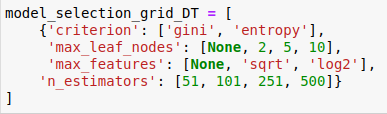
\includegraphics[width=0.7\linewidth]{immagini/modelSelectionGridRF}
		\caption{Griglia di iperparametri usata all'interno della fase di \textit{tuning} degli iperparametri mediante la \textit{GridSearchCV}.}
		\label{fig:modelselectiongridrf}
	\end{figure}
	
	%\begin{lstlisting}[frame=single, basicstyle=\footnotesize]
	%	model_selection_grid_DT = [
	%	{'criterion': ['gini', 'entropy'],
	%		'max_leaf_nodes': [None, 2, 5, 10],
	%		'max_features': [None, 'sqrt', 'log2'],
	%		'n_estimators': [51, 101, 251, 500]}
	%	]
	%\end{lstlisting}
	La valutazione della configurazione degli iperparametri è stata fatta usando una \textit{cross-validation} interna a \textit{GridSearchCV}. Nello specifico \textit{GridSearchCV} opera una \textit{Stratified $k$ fold cross-validation} (vedi Paragrafo \ref{cross_validation}) usando un numero di \textit{fold} decisi dall'utente. In particolare sono stati usati $2$ \textit{fold} poiché il costo computazionale, alzando il numero di \textit{fold} interni, si alzava enormemente avendo già $10$ \textit{fold} esterni (vedi Paragrafo successivo). 

	\section{Cross-validation}
	\label{cross_validation}
	Come discusso nel Paragrafo \ref{SupervisedLearning} esistono diverse strategie per effettuare \textit{cross-validation}. Negli esperimenti è stata usata una versione diversa da quelle spiegate; in particolare è stata utilizzata una \textit{Stratified K-Folds cross-validation} sia come \textit{cross-validation} ``esterna'', per stimare quindi la \textit{performance} di un modello e quindi la bontà di generalizzazione, sia ``interna'' (vedi Paragrafo \ref{tuning}). La scelta di questo tipo specifico di \textit{cross-validation} è ritenuta opportuna in quanto si adatta molto bene quando si hanno a disposizione dati sbilanciati, esattamente il nostro caso, come visibile in Figura \ref{fig:distribuzionedati}. Tale tecnica consiste nel dividere il \textit{dataset} in $k$ sotto-insiemi (chiamati \textit{fold}) mantenendo però le proporzioni delle diverse classi presenti nell'insieme di dati. Questo garantisce che tutte le categorie del problema di classificazione vengano rappresentate in ogni \textit{fold} di addestramento e di \textit{test}. A ogni iterazione, un diverso \textit{fold} viene utilizzato come \textit{test set} e gli altri $k-1$ come \textit{training set} per addestrare il modello. Questo processo viene ripetuto $k$ volte, utilizzando un diverso \textit{fold} come \textit{test set} ogni volta. La valutazione del modello viene poi calcolata come media delle performance su tutti i $k$\textit{-fold}.
	Nello specifico è stata usata una \textit{Stratified 10-fold cross validation} (vedi Figura \ref{fig:cross-validation}).
	
	
	\section{Metrica di performance}
	\label{metricaAUPRC}
	Come metrica di performance è stata usata l'area sotto la curva \textit{Precision-Recall} (AUPRC). Questa metrica è comunemente utilizzata in problemi di classificazione binaria, sopratutto in casi in cui la distribuzione delle classi è sbilanciata \cite{davis2006relationship}, ovvero il nostro caso, come visibile in Figura \ref{fig:distribuzionedati}.
	La curva \textit{Precision-Recall} mostra la relazione che sussiste tra la \textit{precision} e la \textit{recall}, la quali sono spiegate nel Paragrafo \ref{Metriche_di_performance}, per diverse soglie di classificazione. 
	Per calcolare la curva \textit{Precision-Recall}, prima si eseguono le predizioni utilizzando un modello di classificazione. Poi, per ogni soglia di classificazione, si calcolano \textit{precision} e \textit{recall}. Si ottiene così una serie di coppie di \textit{precision-recall} per diverse soglie di classificazione. Queste coppie possono essere visualizzate come punti su un piano cartesiano, dove la \textit{recall} viene mostrata sull'asse delle $x$ e la \textit{precision} viene mostrata sull'asse delle $y$. Tracciando una linea che connette tutti i punti, si ottiene la curva \textit{Precision-Recall}. In Figura \ref{fig:mirnaauprcexternalwholedatasetpintrumap} è possibile vederne un esempio.
	
	Un'area elevata sotto la curva rappresenta sia una elevata \textit{recall} sia un'elevata \textit{precision}, dove un'elevata \textit{precision} si riferisce a un basso tasso di falsi positivi e un'elevata \textit{recall} a un basso tasso di falsi negativi. Punteggi elevati per entrambe le metriche indicano che il classificatore restituisce risultati accurati (alta precisione), oltre a restituire la maggior parte di tutti i risultati positivi (alto richiamo).
	
	In genere, è importante avere un equilibrio tra \textit{precision} e \textit{recall} in modo da ottenere una buona \textit{performance} del modello. Tuttavia, a volte è  più importante dare maggiore importanza a una delle due metriche in base alle esigenze specifiche del problema di classificazione. Ad esempio, in un problema medico potrebbe essere più importante identificare il più possibile i veri positivi (alte \textit{recall}), anche a discapito di una \textit{precision} più bassa. In altro contesto, come ad esempio la classificazione di email come spam, potrebbe essere più importante la \textit{precision}, in modo da evitare di classificare come spam email importanti.

	Poiché la curva \textit{Precision-Recall} non utilizza i veri-negativi, essi non influenzeranno i risultati. È possibile quindi utilizzare dati sbilanciati come $98\%$ di esempi negativi e $2\%$ di esempi positivi e il modello si concentrerà su come valuta il $2\%$ di esempi positivi. Se il modello riesce a gestire bene gli esempi positivi allora il valore di AUPRC sarà alto, altrimenti sarà basso. L'AUPRC varia su una scala da 1 a 0. In contesti reali, in particolare quelli medici, la frazione delle osservazioni positive è spesso inferiore a $0.5$, il che significa che il valore di AUPRC sarà di base inferiore rispetto a quello di AUROC (vedi Paragrafo \ref{auroc}). È possibile, per esempio, ottenere un AUROC pari a $0.8$ e un AUPRC pari a $0.3$. Ovviamente a prima vista sembrerebbe meglio ottenere prestazioni di 0.8, anche se il numero più significativo per il problema in questione potrebbe benissimo essere l'AUPRC di $0.3$. 
	
	È un po' più difficile interpretare l'AUPRC rispetto all'AUROC, questo perché la \textit{baseline} per AUROC sarà sempre $0.5$, un classificatore casuale, o un lancio di moneta, porterà a un AUROC di $0.5$. Con AUPRC, invece, la \textit{baseline} è pari alla frazione di positivi \cite{10.1371/journal.pone.0118432}, calcolata come numeri di esempi positivi / numero totali di esempi. Ciò significa che classi diverse hanno \textit{baseline} di AUPRC diverse. Una classe con il $12\%$ di positivi ha un AUPRC di base di $0.12$, quindi ottenere un AUPRC di $0.40$ su questa classe è ottimo. Tuttavia, una classe con il $98\%$ di positivi ha un AUPRC di base di $0.98$, il che significa che ottenere un AUPRC di $0.40$ su questa classe è uno scarso risultato. In questo caso specifico la \textit{baseline} per i dati è $0.122$, ottenuta prendendo tutte le osservazioni positive, ovvero $77$, diviso per il numero di osservazioni totali, ovvero $627$.
	
	Il calcolo del valore di AUPRC per la valutazione della bontà di generalizzazione del modello è stato effettuato in maniera duplice:
	\begin{itemize}
		\item ``interna'': all'interno della \textit{Stratified 10-fold cross validation} a ogni iterazione viene calcolato un valore di AUPRC, salvato in una lista e, al termine delle 10 iterazioni, fatta la media; chiameremo questo tipo di AUPRC ``interna'' poiché calcolata, per $10$ volte, internamente ai \textit{fold};
		\item ``esterna'': a ogni iterazione della \textit{Stratified 10-fold cross validation} le predizioni effettuate dal modello sono salvate in una lista e concatenate con le predizioni delle precedenti iterazioni fino a raggiungere le 10 iterazioni date dai $10$ fold. Successivamente le predizioni concatenate sono confrontate con le etichette reali, anch'esse concatenate a ogni iterazione, in maniera complessiva, calcolando così il valore di AUPRC ``esterno'', ovvero calcolato esternamente ai \textit{fold}.
	\end{itemize}

	Gli esperimenti effettuati sono stati una combinazione di tecniche di \textit{dimensionality reduction} come \textit{feature selection}, \textit{feature extraction} o altre tecniche come \textit{t-SNE} (vedi Paragrafo \ref{t-sne}), applicati singolarmente o una a seguito dell'altra sui vari \textit{dataset} illustrati nel Capitolo \ref{Dataset}, quali: proteine, CNV, miRNA e mRNA presi singolarmente, concatenazione di tutti e quattro (\textit{Whole\_dataset}) o concatenazione di alcuni (proteine+miRNA e proteine+miRNA+mRNA). Di seguito sono stati illustrati i risultati ottenuti con particolare attenzione a quelli migliori. Il modello utilizzato è stato sempre \textit{random forest}, illustrato nel Paragrafo \ref{RandomForest}.
	
	\section{Risultati ottenuti}
	\label{risultati}
	Nelle tabelle che seguono, ogni riga corrisponde a una tecnica di \textit{dimensionality reduction} o alla concatenazione di più tecniche applicate una a seguito dell'altra. Il primo valore indica l'AUPRC calcolata ``internamente'' mentre il secondo ``esternamente'' (vedi Paragrafo precedente). Le colonne indicano invece i vari \textit{dataset} utilizzati negli esperimenti illustrati nel Capitolo \ref{Dataset} con l'aggiunta di \textit{Whole\_dataset}, concatenazione di tutti i dataset precedenti, dopo aver normalizzato i dati e scartato le \textit{feature} con una variabilità estremamente bassa, ovvero $0.05$. 
	La fase di filtraggio delle \textit{feature} descritta in precedenza non è stata però applicata al dataset CNV. 
	
	La Tabella \ref{firstExperiments} che segue mostra gli esperimenti effettuati sui diversi \textit{dataset}, mentre in Figura \ref{fig:mannwhitneyuwithumapauprcinternal} è possibile vedere il grafico delle curve di \textit{precision/recall} calcolate sui 10 \textit{fold}, quindi ``internamente'', del miglior risultato ottenuto, usando il \textit{dataset} mRNA e come tecniche \textit{Mannwhitney+Umap} usando $50$ come numero di \textit{feature} estratte attraverso la seconda tecnica. Usando la tecnica di \textit{feature selection} \textit{mRMR} sono invece state selezionate 100 \textit{feature}.
	
	\begin{table}[h]
		\begin{center}
			\begin{adjustbox}{max width=\textwidth}
				\begin{tabular}{lrrrrr}
					\toprule
					{} &    miRNA &  Proteins &  mRNA &  Whole\_dataset & CNV \\
					\midrule
					mannwhitneyu &  \textbf{0.25}, \textbf{0.16} & \textbf{0.23}, \textbf{0.15} & \textbf{0.23}, 0.15 & \textbf{0.23},\textbf{ 0.16} &\textbf{0.13},0.10 \\ 
					mannwhitneyu\_with\_umap  &  \textbf{0.27}, 0.12 & \textbf{0.26}, 0.12 &  \cellcolor{orange}\textbf{0.40}, \textbf{0.14} & 0.\textbf{21}, 0.11 &\textbf{0.27}, \textbf{0.15} \\
					boruta  & \textbf{0.18}, \textbf{0.14}& \textbf{0.17}, 0.12& \textbf{0.20}, \textbf{0.16} & \textbf{0.22}, \textbf{0.16} & -1\\
					mic  &  \textbf{0.25}, \textbf{0.18} &\textbf{0.21}, \textbf{0.16} &\textbf{0.23}, \textbf{0.17} & -1 & \textbf{0.15}, 0.11\\
					mrmr & \textbf{0.20}, \textbf{0.14} &  \textbf{0.19}, \textbf{0.14}  & -1 &  -1 & -1\\
					spearman &\textbf{0.17}, \textbf{0.16} & \textbf{0.21}, \textbf{0.14}& \textbf{0.18}, \textbf{15}& \textbf{0.19}, \textbf{0.20}& \textbf{0.13}, 0.10\\
					\bottomrule
				\end{tabular}
			\end{adjustbox}
		\end{center}
	\caption{Tabella che riassume i valori di AUPRC calcolati sia ``internamente'', primo valore, che ``esternamente'', secondo valore. Dove è presente $-1$ significa che, utilizzando le corrispondenti tecniche, il calcolo non è mai arrivato a convergenza dopo giorni di calcolo, si è deciso quindi di fermare la computazione. In arancione è evidenziato il valore massimo ottenuto mentre in grassetto tutti i valori maggiori della \textit{baseline} di $0.12$.}
	\label{firstExperiments}
	\end{table}

	
	\begin{figure}[h!]
		\centering
		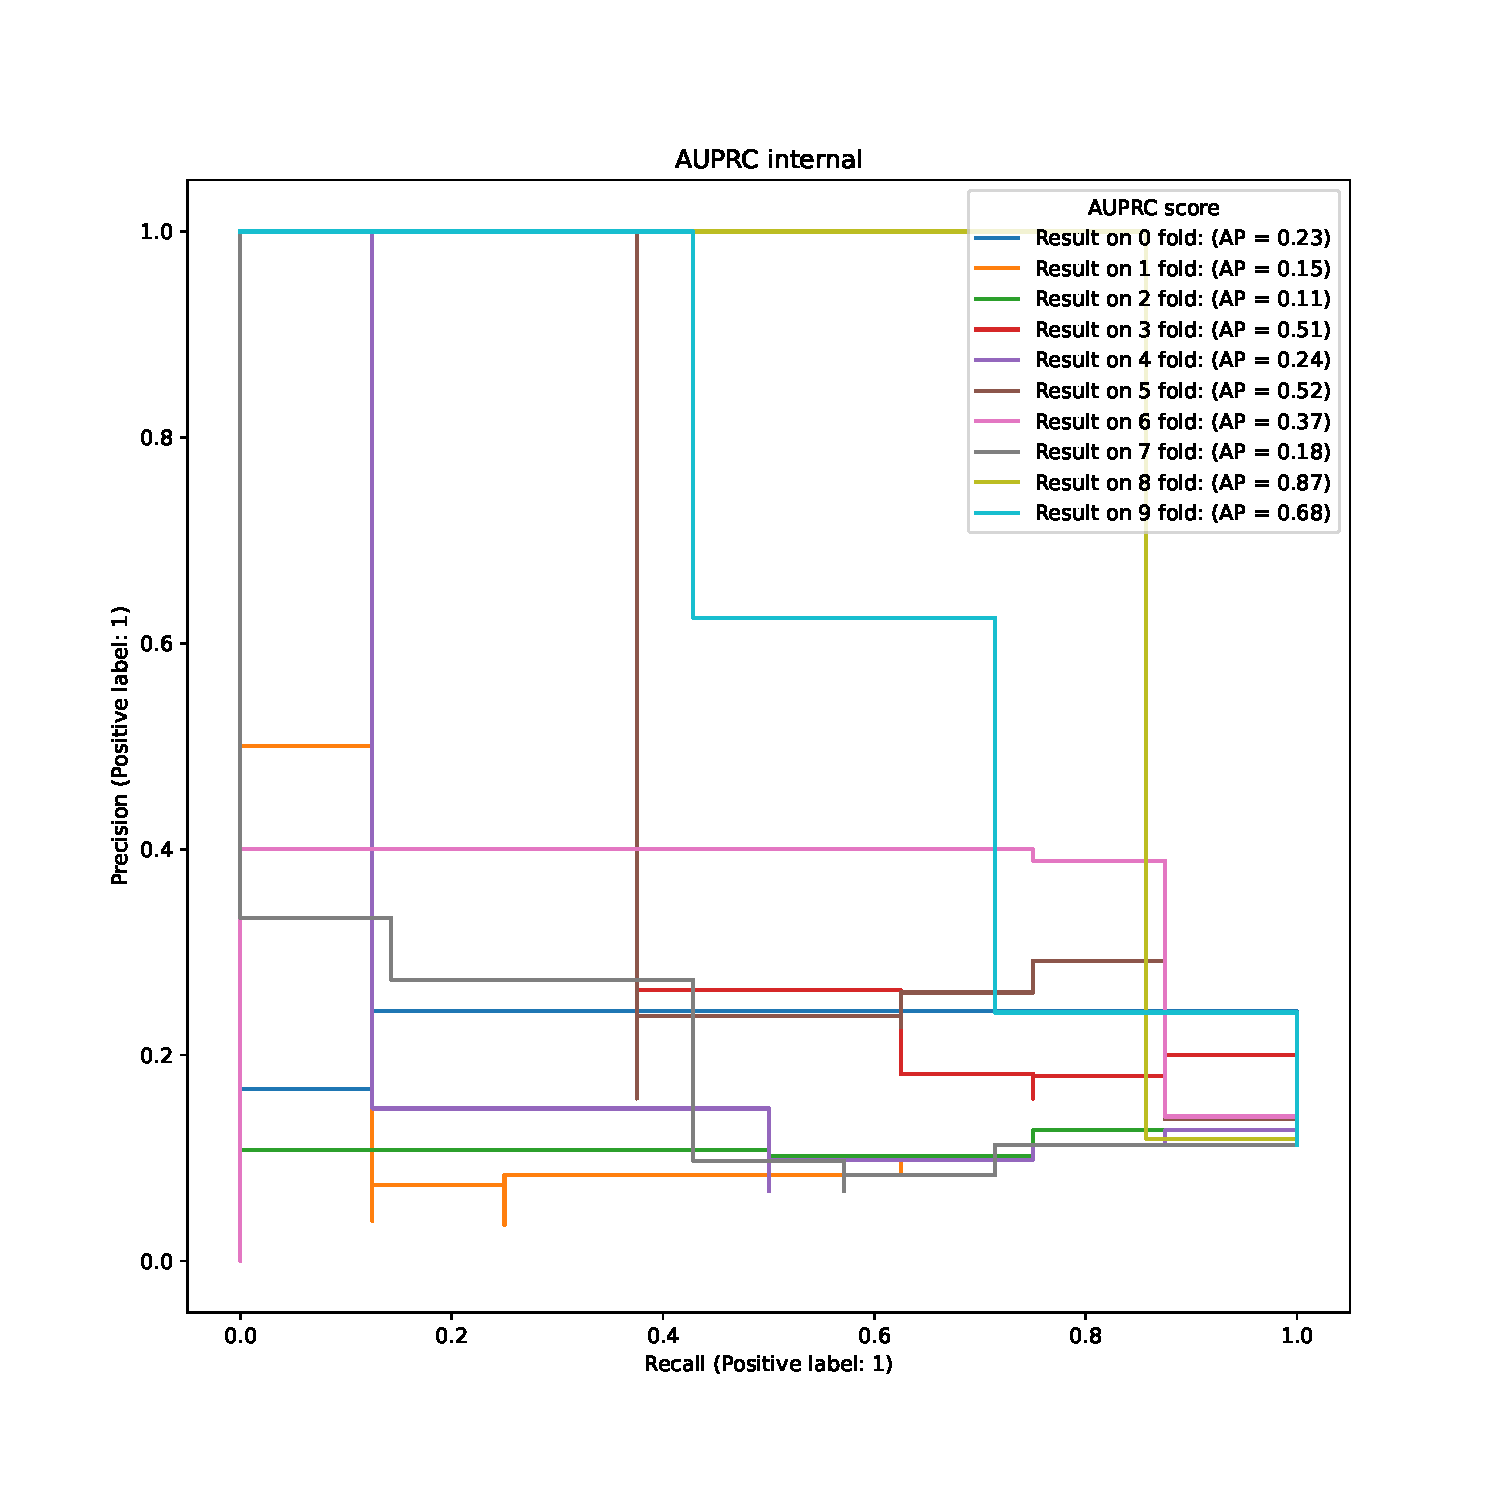
\includegraphics[width=1\linewidth]{immagini/mannwhitneyu_with_umap_AUPRC_Internal}
		\caption{Grafico delle curve di \textit{precision/recall} calcolate sui 10 \textit{fold}, quindi ``internamente'', del miglior risultato ottenuto, usando il \textit{dataset} mRNA e come tecniche \textit{Mannwhitney+Umap}.}
		\label{fig:mannwhitneyuwithumapauprcinternal}
	\end{figure}
	In questo esperimento la migliore configurazione di iperparametri selezionata dalla \textit{GridSearch} è la seguente:
	\begin{itemize}
		\item \textit{max\_leaf\_nodes = } 10,
		\item \textit{n\_estimators = } 51.
	\end{itemize}

	Successivamente si sono svolti ulteriori esperimenti: questa volta inizialmente applicando una tecnica di \textit{feature selection} utilizzando come metrica \textit{Pearson} (vedi Paragrafo \ref{Pearson}) con un \textit{cut-off} di $0.8$. 
	In Tabella \ref{dimPostPearson} è possibile vedere le dimensioni prima e dopo l'applicazione di \textit{Pearson}.

	\begin{table}[h]
		\begin{center}
			\begin{adjustbox}{max width=\textwidth}
				\begin{tabular}{lrrr}
					\toprule
					{} &    prima &  dopo & \textit{feature} scartate\\
					\midrule
					proteins & 216 &216 &0 \\
					mRNA & 18465 & 18411 & 54\\
					miRNA  & 773 & 761 & 12\\
					CNV & 24776 & 194 & 24582 \\
					Whole\_dataset & 44230 & 20386 & 23844\\ 
					proteins+miRNA &989 & 977 & 12 \\
					proteins+miRNA+mRNA & 19454 & 19344 & 110\\
					\bottomrule
				\end{tabular}
			\end{adjustbox}
		\end{center}
		\caption{Tabella che mostra le dimensioni prima e dopo aver filtrato le \textit{feature} usando \textit{Pearson} come indice di correlazione per fare \textit{feature selection}.}
		\label{dimPostPearson}
	\end{table}
	Nella Tabella \ref{AUPRC_on_fold} è, invece, possibile vedere i risultati ottenuti.
	
	
	\begin{table}[h!]
		\begin{center}
			\begin{adjustbox}{max width=\textwidth}
				\begin{tabular}{lrrrrrrr}
					\toprule
					{} &    miRNA &  Proteins &  mRNA &  Whole\_dataset & CNV & Prot+miRNA & Prot+miRNA+mRNA\\
					\midrule
					P+intr+umap & \textbf{0.38}, \textbf{0.18} & \textbf{0.35}, \textbf{0.14}& \textbf{0.32}, \textbf{0.21}& \textbf{0.27}, \textbf{0.17}& \textbf{0.20}, \textbf{0.15}& \cellcolor{orange}\textbf{0.43}, \textbf{0.14}& \textbf{0.38}, \textbf{0.13} \\
					P+intr+tnse & \textbf{0.16}, 0.12 & \textbf{0.20}, \textbf{0.14} & \textbf{0.19}, \textbf{0.13} & \textbf{0.16}, \textbf{0.14} & \textbf{0.16}, \textbf{0.11} & \textbf{0.18}, \textbf{0.12} & \textbf{0.16}, 0.12 \\
					P+mann+boruta & \textbf{0.17}, \textbf{0.13} & \textbf{0.22}, \textbf{0.15} & \textbf{0.23}, \textbf{0.18} &\textbf{0.22}, \textbf{0.15} & -1 & \textbf{0.16}, \textbf{0.13} & \textbf{0.21}, \textbf{0.15 }\\
					P+mann+mrmr & \textbf{0.23}, \textbf{0.17}&\textbf{0.21}, \textbf{0.16} & -1&-1 &\textbf{0.16}, 0.11 & \textbf{0.22}, \textbf{0.16} &-1 \\
					P+mann &\textbf{0.23}, \textbf{0.17}& \textbf{0.21}, \textbf{0.15}& \textbf{0.21}, \textbf{0.16} & \textbf{0.22}, \textbf{0.17} & \textbf{0.16}, 0.12& \textbf{0.25}, \textbf{0.17} & \textbf{0.24}, \textbf{0.18}\\
					\bottomrule
				\end{tabular}
			\end{adjustbox}
		\end{center}
	\caption{Tabella che riassume i valori di AUPRC calcolati sia ``internamente'', primo valore, che ``esternamente'', secondo valore. Dove è presente $-1$ significa che, utilizzando le corrispondenti tecniche, il calcolo non è mai arrivato a convergenza dopo giorni di calcolo, si è preferito quindi fermare la computazione. $P$ sta per \textit{Pearson} (vedi Paragrafo \ref{Pearson}), $intr$ indica l'applicazione della \textit{intrinsic dimensionality} (vedi Paragrafo \ref{IntrinsicDimension}), \textit{mann} indica l'applicazione di  \textit{Mannwhitney} (vedi Paragrafo \ref{Mannwhitney}), la prima tecnica è stata applicata all'intero \textit{dataset} mentre le restanti sono state applicate \textit{on fold}. In arancione è evidenziato il valore massimo ottenuto mentre in grassetto tutti i valori maggiori della \textit{baseline} di $0.12$.}
	\label{AUPRC_on_fold}
	\end{table}

	In questi esperimenti la tecnica di \textit{feature selection}, usando come metrica \textit{Pearson}, è stata applicata al \textit{dataset} completo prima di essere dato in \textit{input} alla funzione che applica una \textit{Stratified 10-fold cross validation}. Successivamente le restanti tecniche di \textit{feature selection} e \textit{dimensionality reduction} sono state applicate \textit{on-fold}, ovvero internamente al \textit{fold} generato. Nello specifico per quanto riguarda il calcolo della dimensionalità intrinseca viene effettuato attraverso l'algoritmo TWO-NN (vedi Paragrafo \ref{two-nn}) applicato sul \textit{training set} del \textit{fold}. La dimensione ottenuta viene poi utilizzata come dimensione obiettivo per il calcolo di \textit{UMAP} e \textit{t-SNE} sia del \textit{training set} che del \textit{test set}.
	
	Per quanto riguarda invece gli altri 3 esperimenti:
	\begin{itemize}
		\item viene applicato \textit{Mannwhitney} sempre \textit{on fold} e le dimensioni selezionate a ogni iterazione vengono salvate per essere usate nei restanti due esperimenti;
		\item alle \textit{feature} selezionate da \textit{Mannwhitney} viene applicato in cascata \textit{boruta} (vedi Paragrafo \ref{boruta}) sempre \textit{on fold};
		\item alle \textit{feature} selezionate da \textit{Mannwhitney} viene applicata in cascata \textit{mRMR} (vedi Paragrafo \ref{mrmr}) sempre \textit{on fold}, usando 100 \textit{feature} come obiettivo.
	\end{itemize}
	
	In Figura \ref{fig:proteinsmirnaauprcinternalmaxresulton-fold} è possibile vedere le  diverse curve di \textit{precision-recall} calcolate sui $10$\textit{-fold} per il miglior risultato ottenuto ovvero usando il \textit{dataset} concatenato così composto: proteine+miRNA. Le tecniche di riduzione della dimensionalità sono invece state: Pearson+calcolo dimensionalità intrinseca+umap a seguire. 
	In questo esperimento la miglior configurazione di iperparametri tra i $10$ diversi addestramenti effettuati nei $10$ fold è:
	\begin{itemize}
		\item \textit{criterion} = \textit{entropy},
		\item \textit{max\_features} = $log_2$,
		\item \textit{max\_leaf\_nodes} = 5,
		\item \textit{n\_estimators}=51.
	\end{itemize}
	
	\begin{figure}[h!]
		\centering
		\includegraphics[width=0.9\linewidth]{"immagini/proteins_mirna_AUPRC_Internal_max_result_on _fold"}
		\caption{Grafico delle curve di \textit{precision/recall} calcolate sui $10$ \textit{fold}, quindi ``internamente'', del miglior risultato ottenuto, usando il \textit{dataset} proteine+miRNA e come tecniche \textit{Pearson}+calcolo dimensionalità intrinseca+umap.}
		\label{fig:proteinsmirnaauprcinternalmaxresulton-fold}
	\end{figure}
	
	Infine sono stati eseguiti ulteriori esperimenti: la tipologia è identica a quella illustrata sopra ma questa volta tutte le tecniche di \textit{feature selection} e \textit{dimensionality reduction} sono state applicate sul \textit{dataset} completo, non sul \textit{fold}. 
	In Tabella \ref{dimPostPearson} è possibile vedere le dimensioni prima e dopo l'applicazione di \textit{Pearson}. 
	
	In Tabella \ref{AUPRC_whole_dataset} è possibile vedere i risultati. Nelle Figure  \ref{fig:mirnaauprcexternalwholedatasetpintrumap} e \ref{fig:mirnaauprcinternalwholedatasetpintrumap} invece è possibile vedere la curva \textit{precision/recall} del migliore addestramento ottenuto rispettivamente ``esternamente'' e ``internamente''. 
	
	\begin{table}[h]
		\begin{center}
			\begin{adjustbox}{max width=\textwidth}
				\begin{tabular}{lrrrrrrr}
					\toprule
					{} &    miRNA &  Proteins &  mRNA &  Whole\_dataset & CNV & Prot+miRNA & Prot+miRNA+mRNA\\
					\midrule
					P+intr+umap & \cellcolor{orange}\textbf{0.78}, \textbf{0.78}& \textbf{0.71}, \textbf{0.70}& \textbf{0.63}, \textbf{0.64}& \textbf{0.68}, \textbf{0.66}&\textbf{0.55}, \textbf{0.56}&\textbf{0.74}, \textbf{0.74} &\textbf{0.70}, \textbf{0.68}  \\
					P+intr+tnse & \textbf{0.21}, \textbf{0.15}& \textbf{0.14}, 0.11 &\textbf{0.17}, 0.11 &\textbf{0.16}, \textbf{0.14}  &\textbf{0.15}, 0.12 & \textbf{0.19}, \textbf{0.14} & \textbf{0.18}, \textbf{0.14} \\
					P+mann+boruta &\textbf{0.29}, \textbf{0.18}  & \textbf{0.24}, \textbf{0.17} & \textbf{0.38}, \textbf{0.29} &\textbf{0.39}, \textbf{0.30} & -1 & \textbf{0.30}, \textbf{0.24} & \textbf{0.38}, \textbf{0.32} \\
					P+mann+mrmr &\textbf{0.25}, \textbf{0.18} & \textbf{0.23}, \textbf{0.17} & -1 & -1 & \textbf{0.29}, \textbf{0.16} & \textbf{0.29}, \textbf{0.22} & -1\\
					P+mann & \textbf{0.22}, \textbf{0.18} & \textbf{0.25}, \textbf{0.19} & \textbf{0.26}, \textbf{0.18} & \textbf{0.26}, \textbf{0.16} & \textbf{0.24}, \textbf{0.17} & \textbf{0.31}, \textbf{0.21} & \textbf{0.25}, \textbf{0.17}\\
					\bottomrule
				\end{tabular}
			\end{adjustbox}
		\end{center}
	\caption{Tabella che riassume i valori di AUPRC calcolati sia ``internamente'', primo valore, che ``esternamente'', secondo valore. Dove è presente $-1$ significa che, utilizzando le corrispondenti tecniche, il calcolo non è mai arrivato a convergenza dopo giorni di calcolo, e si è preferito quindi fermare il calcolo. $P$ sta per \textit{Pearson} (vedi Paragrafo \ref{Pearson}), $intr$ indica l'applicazione della \textit{intrinsic dimensionality}  (vedi Paragrafo \ref{IntrinsicDimension}), \textit{mann} indica l'applicazione di \textit{Mannwhitney} (vedi Paragrafo \ref{Mannwhitney}), tutte le tecniche sono state applicate sull'intero \textit{dataset}. In arancione è evidenziato il valore massimo ottenuto mentre in grassetto tutti i valori maggiori della \textit{baseline} di $0.12$ (vedi Paragrafo \ref{metricaAUPRC}).}
	\label{AUPRC_whole_dataset}
	\end{table}

	In Figura \ref{fig:confusionmatrixbestresult} è possibile vedere la matrice di confusione del miglior risultato ottenuto ``esternamente'' ($0.78$). Essa mostra come il classificatore non sbagli mai a classificare pazienti sani (su 550 pazienti sani vengono classificati tutti come tali). Per quanto riguarda invece i pazienti malati, su 77 totali, 23 ($30\%$) vengono classificati sani (basso sinistra), sbagliando, mentre 54 ($70\%$) vengono classificati malati (basso sinistra), non sbagliando. In Figura \ref{fig:mirnaaurocexternalwholedatasetpintrumap} è possibile vedere invece il calcolo della AUROC (vedi Paragrafo \ref{auroc}).

	
	
	\begin{figure}[h]
		\centering
		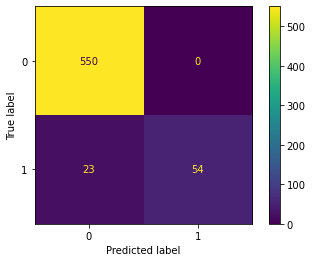
\includegraphics[width=0.7\linewidth]{immagini/ConfusionMatrixBestResult}
		\caption{Matrice di confusione del miglior risultato di AUPRC calcolato ``esternamente'' ottenuto dagli esperimenti ($0.78$). Sull'asse $x$ troviamo le predizioni fatte dal classificatore mentre sull'asse $y$ troviamo le etichette corrette. 1 indica un paziente malato, 0 un paziente sano.}
		\label{fig:confusionmatrixbestresult}
	\end{figure}
	

	\begin{figure}[h]
		\centering
		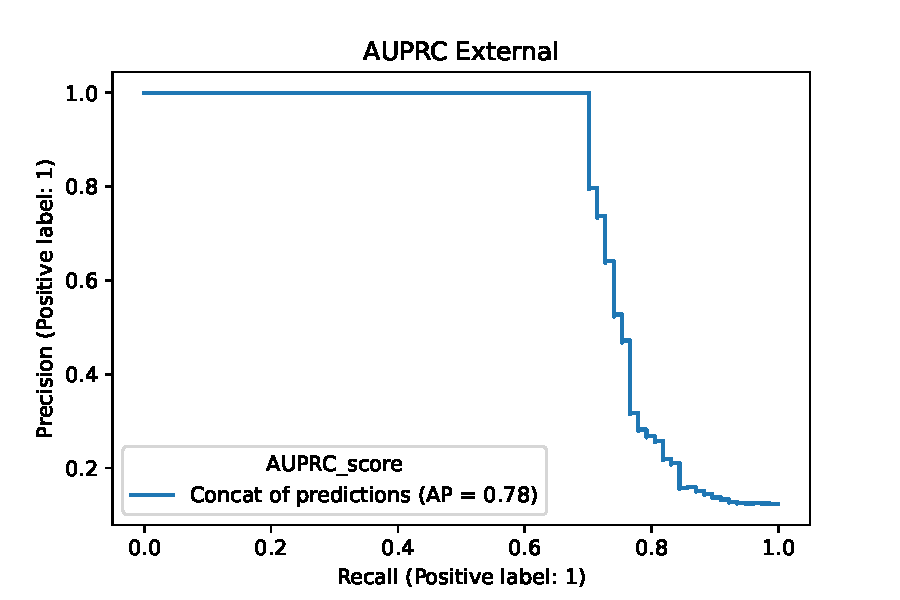
\includegraphics[width=0.7\linewidth]{immagini/mirna_AUPRC_External_whole_dataset_P_intr_umap}
		\caption{Grafico della curva di \textit{precision/recall} calcolata come media delle AUPRC sui 10 \textit{fold} quindi ``esternamente'', del miglior risultato ottenuto, usando il \textit{dataset} miRNA e come tecniche \textit{Pearson}, calcolo della dimensionalità intrinseca e la dimensione ottenuta ($45$) usata nella funzione che calcola \textit{UMAP} a tutto il \textit{dataset}.}
		\label{fig:mirnaauprcexternalwholedatasetpintrumap}
	\end{figure}

	\begin{figure}[h]
		\centering
		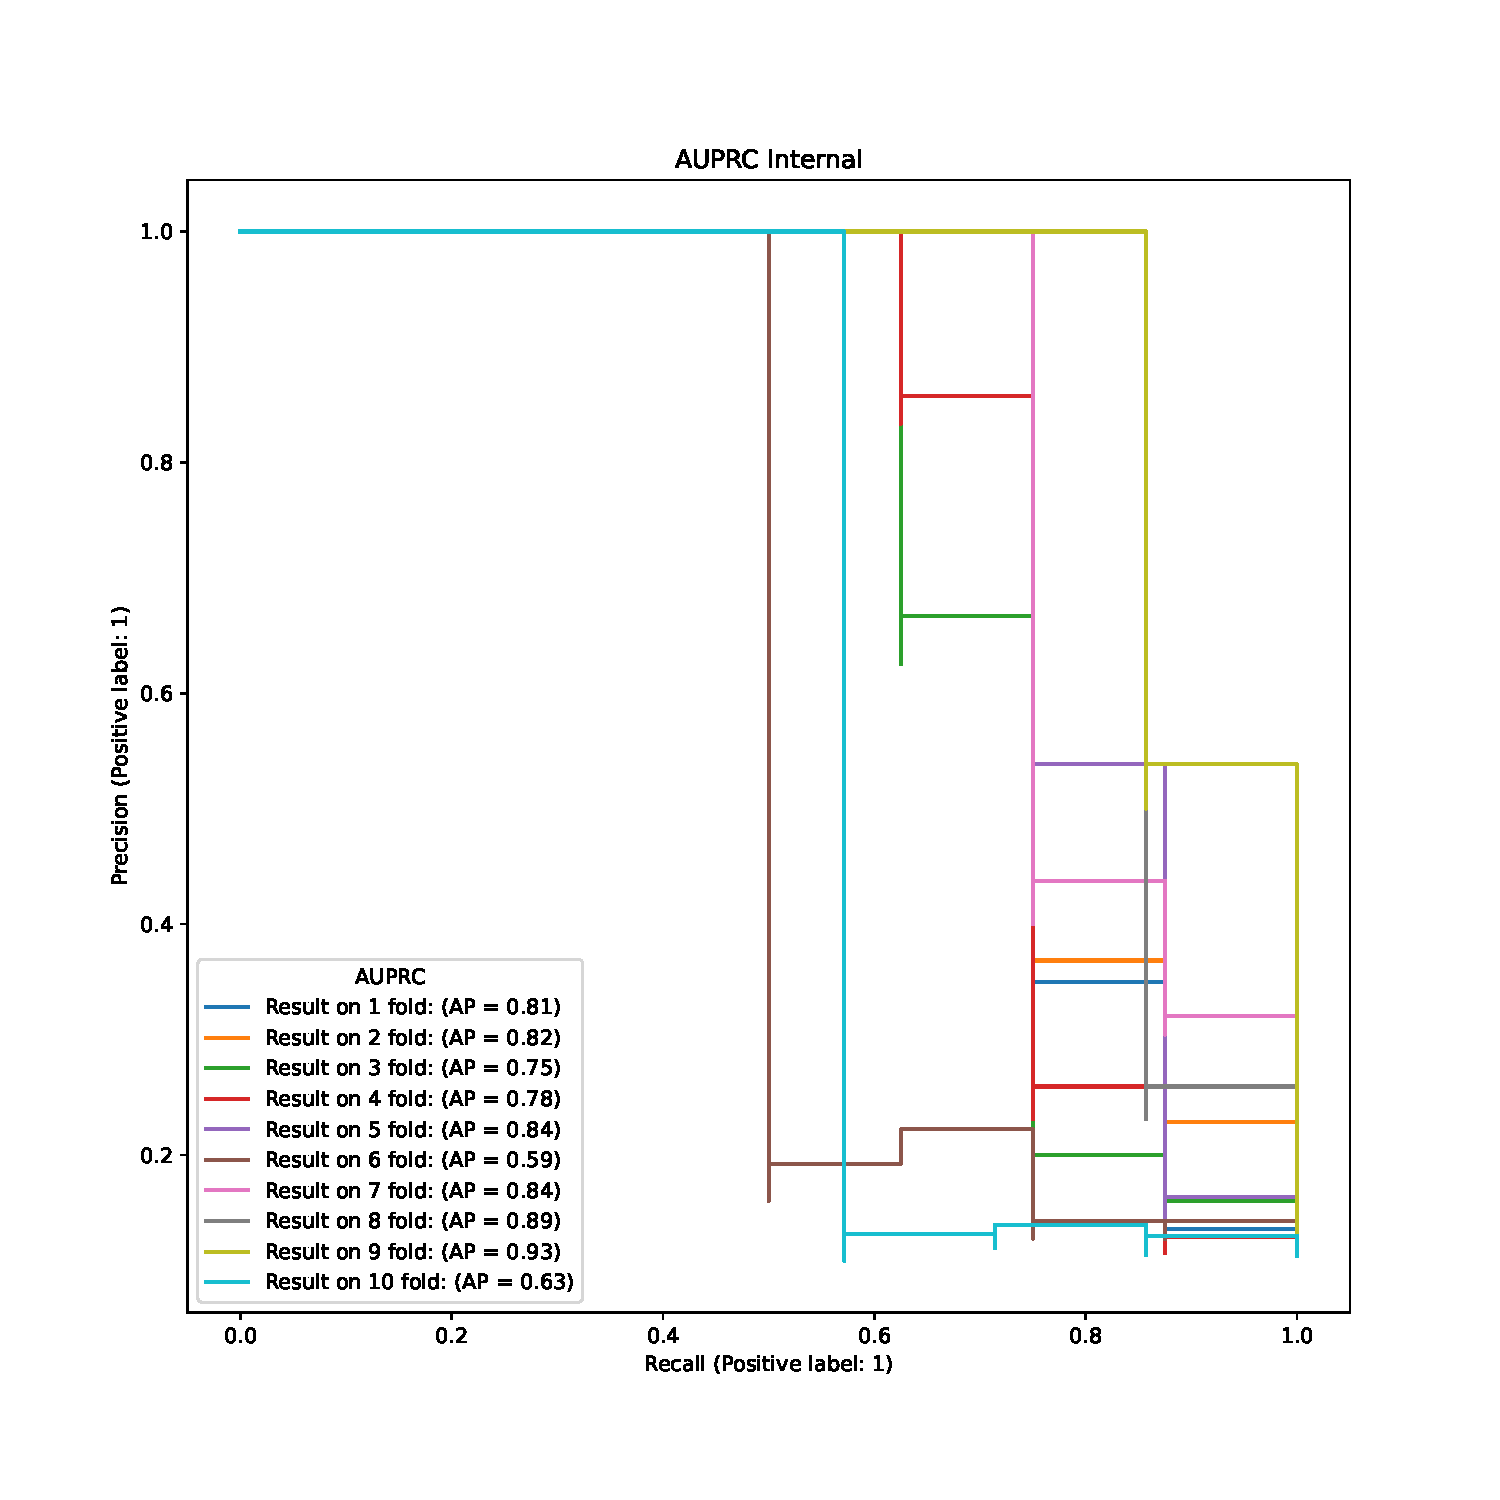
\includegraphics[width=1\linewidth]{immagini/mirna_AUPRC_Internal_whole_dataset_p_intr_umap}
		\caption{Grafico delle curve di \textit{precision/recall} calcolate sui 10 \textit{fold}, quindi ``internamente'', del miglior risultato ottenuto, usando il \textit{dataset} miRNA e come tecniche \textit{Pearson}, calcolo della dimensionalità intrinseca e la dimensione ottenuta usato nella funzione che calcola \textit{UMAP} a tutto il \textit{dataset}.}
		\label{fig:mirnaauprcinternalwholedatasetpintrumap}
	\end{figure}

	\begin{figure}[h]
		\centering
		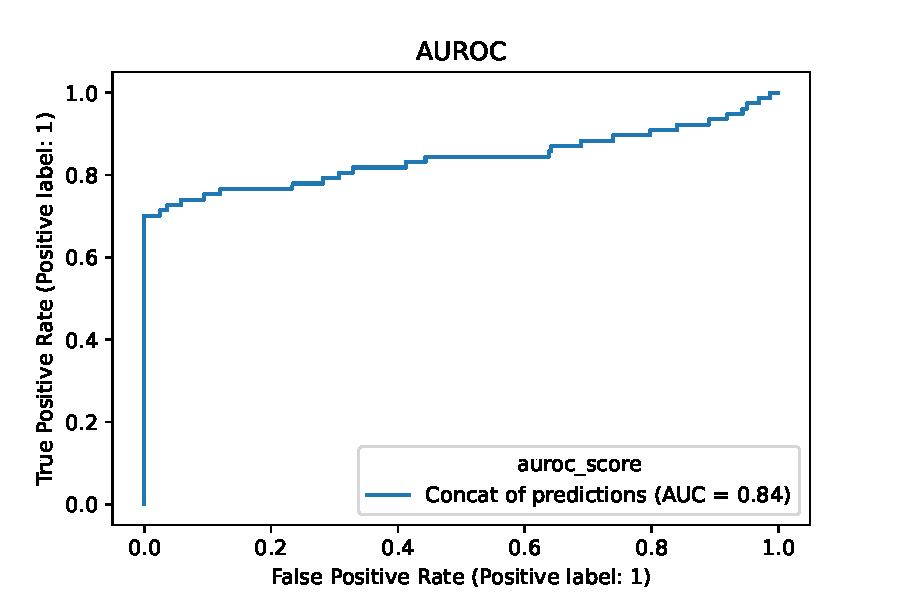
\includegraphics[width=0.7\linewidth]{immagini/mirna_AUROC_External_whole_dataset_p_intr_umap}
		\caption{Grafico della curva ROC, anch'essa calcolata ``esternamente'', del miglior risultato ottenuto, usando il \textit{dataset} miRNA e come tecniche \textit{Pearson}, calcolo della dimensionalità intrinseca e la dimensione ottenuta ( ovvero $45$) usata nella funzione che calcola \textit{UMAP} a tutto il \textit{dataset}.}
		\label{fig:mirnaaurocexternalwholedatasetpintrumap}
	\end{figure}

	Infine in Tabella \ref{classification_report} è possibile vedere valori delle metriche \textit{precision}, \textit{recall}, \textit{F-1-score} per le classi 0 e 1, ovvero rispettivamente sano e malato. È inoltre presente la metrica \textit{support} che rappresenta il numero di esempi di una classe specifica nel \textit{dataset}. In questo caso quindi ci sono $550$ esempi negativi e $77$ positivi.
	
	Inoltre questo addestramento ha un valore di \textit{specificity} pari a $1.0$. Per quanto riguarda invece la configurazione di iperparametri la migliore è la seguente:
	\begin{itemize}
		\item \textit{max\_features} = None,
		\item \textit{max\_leaf\_nodes} = 10,
		\item \textit{n\_estimators}=251.
	\end{itemize}
	\begin{table}[h]
		\centering
		\begin{tabular}{lrrrr}
			\toprule
			{} & Precision & Recall & f1-score & support \\ \midrule
			class 0 & 0.96 & 1.00 & 0.98 & 550  \\
			class 1 & 1.00 & 0.70 & 0.82 & 77 \\
			\bottomrule
		\end{tabular}
		\caption{Tabella che mostra i valori di \textit{precision, recall, f1-score e support}. \textit{Class 0} indica la classe dei pazienti sani mentre \textit{class 1} indica la classe dei pazienti malati.}
		\label{classification_report}
	\end{table}
	

	\clearpage
	
	\section{Analisi dei risultati}
	Osservando la Tabella \ref{firstExperiments} è possibile vedere che i primi esperimenti non presentano un valore di AUPRC elevato. Va però ricordata l'osservazione sulla \textit{baseline} fatta nel Paragrafo \ref{metricaAUPRC}. Come detto precedentemente in questo caso la \textit{baseline} è di $0.12$ quindi valori superiori a questa quantità sono da considerarsi positivi. In ogni caso non c'è stato un esperimento con esito estremamente positivo. Il valore massimo di AUPRC ottenuto è stato $0.40$ usando come \textit{dataset} mRNA e come tecniche \textit{Mannwhitney} e \textit{UMAP} a seguire, il valore è stato ottenuto calcolando l'AUPRC internamente. In Tabella \ref{firstExperiments} sono visibili anche valori pari a $-1$, questo indica che il calcolo non è mai riuscito a convergere. Ciò è causato dall'alto numero di dimensioni del dataset mRNA, circa $20.000$ e di conseguenza da \textit{Whole\_dataset}, composto dalla concatenazione di tutti i \textit{dataset}.
	
	Per quanto riguarda gli esperimenti effettuati i cui esiti sono visibili in Tabella \ref{AUPRC_on_fold} i valori di AUPRC sono mediamente più elevati rispetto agli esperimenti precedenti. Questi esperimenti sono stati effettuati applicando prima \textit{Pearsom} sull'intero \textit{dataset}. Successivamente è stata calcolata la dimensionalità intrinseca e la dimensione ottenuta usata come dimensione obiettivo per UMAP, queste tecniche sono state applicate \textit{on fold}. L'addestramento migliore ha portato a un valore di AUPRC di $0.43$ usando il \textit{dataset} proteine+miRNA. Anche in questo caso il valore viene calcolato ``internamente''.
	In Tabella \ref{AUPRC_on_fold}, come nella precedente, è possibile trovare valori pari a $-1$ e questo è dovuto allo stesso motivo sopra citato.
	
	Infine, in Tabella \ref{AUPRC_whole_dataset}, è possibile vedere i risultati ottenuti usando le tecniche sull'intero \textit{dataset} e non \textit{on fold}. Complessivamente sono i risultati migliori di tutti gli esperimenti e in particolare troviamo ottimi risultati ottenuti usando come tecniche: \textit{Pearson+intrinsic dimensionality} e \textit{UMAP} a seguire. Su tutti i \textit{dataset} questa combinazione porta a ottimi risultati, quello migliore in assoluto è stato ottenuto usando come \textit{dataset} miRNA ottenendo $0.78$ e $0.78$, calcolando l'AUPRC, rispettivamente, ``internamente'' ed ``esternamente''.
	In Figura \ref{fig:confusionmatrixbestresult} è mostrata la matrice di confusione dell'addestramento il cui valore di AUPRC è calcolato ``esternamente''. Essa mostra come il classificatore classifichi come sani tutti i pazienti che effettivamente lo sono ($550$ su $550$). Per quanto riguarda invece i malati, su $77$ pazienti: $54$ (ovvero il $70\%$) vengono classificati come malati, in maniera corretta, mentre i restati $23$ pazienti vengono classificati come sani, sbagliando.
	
	
	Complessivamente possiamo accorgerci di come il calcolo dell'AUPRC eseguito ``internamente'' porti a valori più elevati nella maggior parte dei casi. Inoltre è bene notare come in tutte le tabelle i risultati migliori siano sempre ottenuti usando \textit{UMAP} come tecnica di riduzione della dimensionalità.
	
	\section{Tecnologie usate}
	Per eseguire questo studio sono state utilizzate diverse tecnologie, prima tra tutte il linguaggio usato è stato \textit{Python} 3.10.6, unitamente a diversi pacchetti specifici per l'analisi dei dati quali: \textit{pandas} e \textit{numpy}. Pacchetti per applicare le tecniche di riduzione della dimensionalità quali: \textit{scipy}, \textit{umap}, \textit{minepy}, \textit{pymrmr} e \textit{boruta}. Infine \textit{sklearn} per l'applicazione specifica di tecniche di apprendimento automatico.
	Come ambiente di lavoro è stato usato \textit{Jupyter Notebook}, mentre come tool di \textit{versioning}, \textit{git} unitamente a \textit{github}. 
	
	\chapter{Conclusioni}
	\label{Conclusioni}
	In questo lavoro è stato sviluppato un modello di predizione usando dati provenienti dai geni BRCA in modo da predire diagnosi e prognosi del carcinoma mammario invasivo per nuovi pazienti. In particolare si voleva analizzare se l'utilizzo di dati multi-omici aumentasse la precisione di classificazione usando l'algoritmo di apprendimento supervisionato \textit{random forest}. La scelta è ricaduta su questo algoritmo poiché famoso in letteratura per essere uno dei migliori quando si utilizzano dati eterogenei perché utilizza una foresta di \textit{decision tree} in cui ogni albero è formato da decisioni basate su diverse caratteristiche.
	
	Inizialmente sono state studiate e visionate alcune soluzioni simili in campo medico. In particolare studi sull'applicazione di apprendimento supervisionato per la predizione di malattie associate a varianti non codificanti e	riguardanti la previsione di rischio di COVID-19 nei pazienti \cite{Schubach2017, Casiraghi2020-zt}.
	
	I dati usati sono stati presi da \textit{The Cancer Genome Atlas} (TCGA), programma scientifico di riferimento per la genomica del cancro. Per quanto riguarda invece le etichette sono state prese da un \textit{dataset} curato manualmente, noto come TCGA-CDR. Esso indica la presenza o assenza di evento tumorale in un paziente.
	I dati forniti contenevano valori nulli. Pertanto sono state eliminate le \textit{feature} che contenevano un numero di valori nulli superiore al $20\%$, dopo questa scrematura non è stato necessario adottare tecniche di imputazione poiché non sono rimasti ulteriori dati di questo tipo. Successivamente i dati sono stati normalizzati a un valore compreso tra 0 e 1.
	Infine sono state scartate \textit{feature} con una variabilità inferiore a $0.05$ poiché poco informative. 
	A seguito di questa prima pulizia dei dati, sono state applicate tecniche di riduzione della dimensionalità poiché un numero di \textit{feature} troppo elevato all'interno dei \textit{dataset} porta a un significativo rallentamento degli algoritmi di apprendimento automatico, peggioramento della \textit{performance} predittiva degli stessi algoritmi e difficoltà nell'interpretazione del modello. Queste tecniche sono state applicate sia singolarmente (vedi Tabella \ref{firstExperiments}) che concatenando più tecniche (vedi Tabelle \ref{AUPRC_on_fold} e \ref{AUPRC_whole_dataset}). Le tecniche sono state applicate sia ai singoli \textit{dataset} (\textit{proteins, miRNA, mRNA e CNV}), sia a \textit{dataset} derivati dalla concatenazione dei precedenti (dati multi-omici come: \textit{whole\_dataset, proteins+miRNA e proteins+miRNA+mRNA}). La metrica usata sia per valutare la bontà di generalizzazione del modello sia per eseguire il \textit{tuning} degli iperparametri è stata l'AUPRC (\textit{Area Under the Precision-Recall Curve}). Questa metrica è comunemente utilizzata in problemi di classificazione binaria, sopratutto quando la distribuzione dei dati è sbilanciata, ovvero esattamente il nostro caso, come visibile in Figura \ref{fig:distribuzionedati}. Il valore di AUPRC varia su una scala da 0 a 1. In contesti medici, come quello trattato in questo lavoro, la frazione delle osservazioni positive, ovvero che rappresentano pazienti malati, è spesso inferiore a $0.5$, in questo caso è $0.12$. Questo comporta che la \textit{baseline} di AUPRC, per questo problema di classificazione, è esattamente $0.12$ e valori superiori possono considerarsi buoni.
	
	La maggior parte dei risultati ottenuti hanno un valore di AUPRC superiore alla \textit{baseline} di $0.12$ imposta da come è composto il \textit{dataset} ($550$ pazienti sani, $77$ pazienti malati). Non c'è però evidenza che l'utilizzo di dati multi-omici aumenti la capacità dell'algoritmo \textit{random forest} di classificare in maniera più precisa pazienti sani e pazienti malati. A fronte di questo però ci sono tecniche che ottengono un buon valore di AUPRC, ovvero \textit{Pearson} + calcolo dimensionalità intrinseca usando \textit{Two Nearest Neighbor} (Two-NN) + UMAP impostando come numero di \textit{feature} estratte quello calcolato da Two-NN.
	Questa concatenazione di tecniche ottiene i risultati migliori su ogni tipo di \textit{dataset}, come si può vedere nelle Tabelle \ref{AUPRC_on_fold} e \ref{AUPRC_whole_dataset}. La differenza tra gli esperimenti delle due tabelle risiede in come sono state applicate le tecniche di riduzione della dimensionalità. Nella prima le tecniche sono state applicate \textit{on fold} mentre nella seconda sono state applicate sull'intero \textit{dataset}.
	In particolare è applicando le tecniche sull'intero \textit{dataset} e poi usando il \textit{dataset} ottenuto come \textit{input} per l'algoritmo di apprendimento che si ottengono i risultati migliori, visibili in Tabella \ref{AUPRC_whole_dataset}. Considerando la \textit{baseline} di partenza, ovvero $0.12$, un risultato di $0.78$, utilizzando miRNA, è da considerarsi ottimo. In Figura \ref{fig:confusionmatrixbestresult} è possibile però vedere come il modello classifichi correttamente i dati di \textit{test} dei pazienti sani, ma che su $77$ malati, $54$ vengono classificati come effettivamente malati mentre $23$ pazienti vengono classificati come sani, sbagliando. In campo medico questo fatto non è da considerarsi propriamente ottimo poiché quasi il $30\%$ dei malati vengono classificati non malati, quando in verità lo sarebbero.
	
	\section{Sviluppi futuri}
	
	Questo lavoro presenta alcune limitazioni intrinseche. Prima di tutto scarsità di osservazioni positive dovute allo sbilanciamento tra pazienti sani e malati. Alcune delle possibili soluzioni potrebbero essere quelle di raccogliere ulteriori osservazioni riguardanti pazienti positivi al carcinoma mammario invasivo  anche se in campo medico non è una pratica così facile da realizzare. Un'altra soluzione potrebbe essere quella di adottare tecniche di bilanciamento delle classi, come \textit{Synthetic Minority Over-Sampling Technique} (SMOTE) \cite{chawla2002smote}.
	Inoltre usando alcune tecniche di riduzione della dimensionalità la computazione non è mai arrivata al termine dopo giorni di calcolo, ovvero in corrispondenza dei $-1$ visibili nelle Tabelle \ref{AUPRC_on_fold} e \ref{AUPRC_whole_dataset}.
	L'\textit{hardware} su cui sono stati condotti gli esperimenti è stato un processore molto recente, ovvero un Intel Core i5-13600K \cite{i5-13600k}. Tuttavia, per comprendere pienamente le potenzialità delle tecniche analizzate, sarebbe opportuno, come sviluppo futuro, quello di provare a eseguire ulteriori esperimenti su \textit{hardware} ancora più performante, come ad esempio server dedicati. In questo modo si potrebbero sia utilizzare le tecniche di riduzione della dimensionalità che non riescono a convergere, sia allargare la griglia di iperparametri della \textit{GridSearchCV}. Questo comporterebbe un aumento del costo computazionale ma si potrebbe riuscire a trovare un modello che si adatta meglio ai dati a disposizione e che riesca a ottenere un grado di bontà di generalizzazione superiore a quello ottenuto dai modelli che sono stati usati durante gli esperimenti. 
	Un ulteriore sviluppo futuro possibile potrebbe essere quello di utilizzare algoritmi di apprendimento automatico più complessi, non solo \textit{random forest}, come \textit{artificial neural network} \cite{lisboa2006use} o \textit{XGBoost} \cite{liew2021investigation, kabiraj2020breast, zhang2020novel}.
	
	\clearpage
	%
	%			BIBLIOGRAFIA
	%
	
	\nocite{smlbook}
	\nocite{Kingsford2008}
	\bibliographystyle{unsrt}
	\bibliography{bibliografia}
	\addcontentsline{toc}{chapter}{Bibliografia}
	
\end{document}
